% Supplementary material for the CVPR 2027 submission
% "Last-Meter Precision Navigation for UAVs: A Geometric Imagination-Based Aerial Visual Servoing Approach"
% Build:  pdflatex supp && bibtex supp && pdflatex supp && pdflatex supp
% Tables under tables/ and the macros in numbers.tex are generated from the result files by
% supp/make_tables.py in the code repository; do not edit them by hand.
\documentclass[10pt,twocolumn,letterpaper]{article}
\usepackage[review]{cvpr}
\usepackage{multirow}
\usepackage{makecell}
\usepackage{colortbl}
\usepackage{bm}
\usepackage{array}
\definecolor{cvprblue}{rgb}{0.21,0.49,0.74}
\definecolor{rowgray}{gray}{0.93}
\usepackage[pagebackref,breaklinks,colorlinks,allcolors=cvprblue]{hyperref}

\def\paperID{*****} % TODO(authors): submission ID
\def\confName{CVPR}
\def\confYear{2027}

\title{Last-Meter Precision Navigation for UAVs: A Geometric Imagination-Based\\ Aerial Visual Servoing Approach}
\author{Anonymous CVPR submission}

% ---- numbering that cannot be confused with the main paper
\renewcommand{\thesection}{\Roman{section}}
\renewcommand{\thesubsection}{\thesection.\arabic{subsection}}
\renewcommand{\thetable}{S\arabic{table}}
\renewcommand{\thefigure}{S\arabic{figure}}
\renewcommand{\theequation}{S\arabic{equation}}
\makeatletter
\renewcommand{\p@subsection}{}
\makeatother

% ---- notation
\newcommand{\dth}{\Delta\theta}
\newcommand{\dpsi}{\Delta\psi}
\newcommand{\dpv}{\Delta\mathbf{p}}
\newcommand{\dpvh}{\Delta\hat{\mathbf{p}}}
\newcommand{\lv}{\bm{\ell}}
\newcommand{\SRd}{SR$_{d}$}
\newcommand{\SRe}{SR$_{\mathrm{EPE}}$}
\newcommand{\SRf}{SR$_{\mathrm{5D}}$}
\newcommand{\wrapd}{\ominus}
\newcommand{\ci}[2]{{\scriptsize[\ensuremath{#1},\,\ensuremath{#2}]}}
\newcommand{\best}[1]{\textbf{#1}}
\newcommand{\main}[1]{#1 of the main paper}
\newcommand{\todoauthors}[1]{\textbf{\color{red}[Authors: #1]}}
% generated by supp/make_tables.py
\newcommand{\SiCamD}{0.92}
\newcommand{\SiCamEPEmean}{1.71}
\newcommand{\SiCamEPEmed}{0.82}
\newcommand{\SiCamSRd}{73.1}
\newcommand{\SiCamSRdHi}{74.3}
\newcommand{\SiCamSRdLo}{71.6}
\newcommand{\SiCamSRe}{59.9}
\newcommand{\SiCamSReHi}{61.5}
\newcommand{\SiCamSReLo}{58.2}
\newcommand{\SiCamSRf}{59.2}
\newcommand{\SiCamX}{0.83}
\newcommand{\SiCamY}{0.92}
\newcommand{\SiCamZ}{0.81}
\newcommand{\SiEnuD}{0.92}
\newcommand{\SiEnuEPEmean}{2.42}
\newcommand{\SiEnuEPEmed}{1.14}
\newcommand{\SiEnuSRd}{73.1}
\newcommand{\SiEnuSRdHi}{74.3}
\newcommand{\SiEnuSRdLo}{71.6}
\newcommand{\SiEnuSRe}{44.3}
\newcommand{\SiEnuSReHi}{46.9}
\newcommand{\SiEnuSReLo}{41.8}
\newcommand{\SiEnuSRf}{43.9}
\newcommand{\SiEnuX}{1.37}
\newcommand{\SiEnuY}{1.35}
\newcommand{\SiEnuZ}{0.81}
\newcommand{\SiiCamD}{0.68}
\newcommand{\SiiCamEPEmean}{1.01}
\newcommand{\SiiCamEPEmed}{0.53}
\newcommand{\SiiCamSRd}{83.3}
\newcommand{\SiiCamSRdHi}{84.6}
\newcommand{\SiiCamSRdLo}{81.8}
\newcommand{\SiiCamSRe}{78.7}
\newcommand{\SiiCamSReHi}{80.2}
\newcommand{\SiiCamSReLo}{77.0}
\newcommand{\SiiCamSRf}{78.4}
\newcommand{\SiiCamX}{0.46}
\newcommand{\SiiCamY}{0.50}
\newcommand{\SiiCamZ}{0.54}
\newcommand{\SiiEnuD}{0.68}
\newcommand{\SiiEnuEPEmean}{1.74}
\newcommand{\SiiEnuEPEmed}{0.76}
\newcommand{\SiiEnuSRd}{83.3}
\newcommand{\SiiEnuSRdHi}{84.6}
\newcommand{\SiiEnuSRdLo}{81.8}
\newcommand{\SiiEnuSRe}{61.9}
\newcommand{\SiiEnuSReHi}{64.9}
\newcommand{\SiiEnuSReLo}{58.9}
\newcommand{\SiiEnuSRf}{61.8}
\newcommand{\SiiEnuX}{0.99}
\newcommand{\SiiEnuY}{0.98}
\newcommand{\SiiEnuZ}{0.54}
\newcommand{\baseMaxSRe}{0.0}
\newcommand{\baseMaxYawFree}{1.5}
\newcommand{\baseMaxZ}{19.5}
\newcommand{\baseMinZ}{14.3}
\newcommand{\cfConstD}{6.11}
\newcommand{\cfConstSRd}{7.7}
\newcommand{\cfDinovCamCorr}{0.02}
\newcommand{\cfDinovCamD}{13.05}
\newcommand{\cfDinovCamEPE}{19.1}
\newcommand{\cfDinovCamHor}{7.57}
\newcommand{\cfDinovCamSRd}{3.0}
\newcommand{\cfDinovCamSRe}{0.0}
\newcommand{\cfDinovEnuCorr}{0.01}
\newcommand{\cfDinovEnuD}{12.86}
\newcommand{\cfDinovEnuEPE}{19.2}
\newcommand{\cfDinovEnuHor}{7.83}
\newcommand{\cfDinovEnuSRd}{3.1}
\newcommand{\cfDinowmCamCorr}{\ensuremath{-0.01}}
\newcommand{\cfDinowmCamD}{10.27}
\newcommand{\cfDinowmCamEPE}{23.7}
\newcommand{\cfDinowmCamHor}{8.87}
\newcommand{\cfDinowmCamSRd}{6.1}
\newcommand{\cfDinowmCamSRe}{0.0}
\newcommand{\cfDinowmEnuCorr}{\ensuremath{-0.01}}
\newcommand{\cfDinowmEnuD}{10.33}
\newcommand{\cfDinowmEnuEPE}{23.6}
\newcommand{\cfDinowmEnuHor}{8.94}
\newcommand{\cfDinowmEnuSRd}{6.1}
\newcommand{\cfMaxCamCorr}{0.04}
\newcommand{\cfMaxCamSRd}{8.6}
\newcommand{\cfMaxCamSRe}{0.03}
\newcommand{\cfMinCamD}{7.08}
\newcommand{\cfMlpCamCorr}{0.83}
\newcommand{\cfMlpCamD}{3.15}
\newcommand{\cfMlpCamEPE}{6.1}
\newcommand{\cfMlpCamHor}{3.68}
\newcommand{\cfMlpCamSRd}{21.5}
\newcommand{\cfMlpCamSRe}{0.6}
\newcommand{\cfMlpEnuCorr}{0.07}
\newcommand{\cfMlpEnuD}{5.40}
\newcommand{\cfMlpEnuEPE}{12.2}
\newcommand{\cfMlpEnuHor}{7.44}
\newcommand{\cfMlpEnuSRd}{9.9}
\newcommand{\cfNomadCamCorr}{0.01}
\newcommand{\cfNomadCamD}{7.08}
\newcommand{\cfNomadCamEPE}{25.1}
\newcommand{\cfNomadCamHor}{9.57}
\newcommand{\cfNomadCamSRd}{8.6}
\newcommand{\cfNomadCamSRe}{0.0}
\newcommand{\cfNomadEnuCorr}{\ensuremath{-0.00}}
\newcommand{\cfNomadEnuD}{7.14}
\newcommand{\cfNomadEnuEPE}{25.2}
\newcommand{\cfNomadEnuHor}{9.62}
\newcommand{\cfNomadEnuSRd}{8.6}
\newcommand{\cfSfgCamCorr}{0.01}
\newcommand{\cfSfgCamD}{10.30}
\newcommand{\cfSfgCamEPE}{21.7}
\newcommand{\cfSfgCamHor}{8.58}
\newcommand{\cfSfgCamSRd}{5.7}
\newcommand{\cfSfgCamSRe}{0.0}
\newcommand{\cfSfgEnuCorr}{0.01}
\newcommand{\cfSfgEnuD}{11.00}
\newcommand{\cfSfgEnuEPE}{21.0}
\newcommand{\cfSfgEnuHor}{8.29}
\newcommand{\cfSfgEnuSRd}{5.1}
\newcommand{\cfVfCamCorr}{0.01}
\newcommand{\cfVfCamD}{10.28}
\newcommand{\cfVfCamEPE}{22.9}
\newcommand{\cfVfCamHor}{8.54}
\newcommand{\cfVfCamSRd}{5.7}
\newcommand{\cfVfCamSRe}{0.0}
\newcommand{\cfVfEnuCorr}{\ensuremath{-0.01}}
\newcommand{\cfVfEnuD}{10.30}
\newcommand{\cfVfEnuEPE}{23.0}
\newcommand{\cfVfEnuHor}{8.73}
\newcommand{\cfVfEnuSRd}{5.7}
\newcommand{\cfVintCamCorr}{0.02}
\newcommand{\cfVintCamD}{18.40}
\newcommand{\cfVintCamEPE}{20.1}
\newcommand{\cfVintCamHor}{7.26}
\newcommand{\cfVintCamSRd}{0.2}
\newcommand{\cfVintCamSRe}{0.0}
\newcommand{\cfVintEnuCorr}{\ensuremath{-0.01}}
\newcommand{\cfVintEnuD}{18.91}
\newcommand{\cfVintEnuEPE}{20.0}
\newcommand{\cfVintEnuHor}{7.46}
\newcommand{\cfVintEnuSRd}{0.3}
\newcommand{\cfZeroCamHor}{7.26}
\newcommand{\cfZeroEnuHor}{7.45}
\newcommand{\clDfull}{\ensuremath{+30.0}}
\newcommand{\clDfullHi}{\ensuremath{+35.5}}
\newcommand{\clDfullLo}{\ensuremath{+24.7}}
\newcommand{\clDfullOne}{\ensuremath{+3.0}}
\newcommand{\clDfullOneHi}{\ensuremath{+6.9}}
\newcommand{\clDfullOneLo}{\ensuremath{-0.8}}
\newcommand{\clDfullSiteHi}{\ensuremath{+35.5}}
\newcommand{\clDfullSiteLo}{\ensuremath{+25.3}}
\newcommand{\clDplane}{\ensuremath{+30.5}}
\newcommand{\clDplaneHi}{\ensuremath{+35.2}}
\newcommand{\clDplaneLo}{\ensuremath{+25.6}}
\newcommand{\clDplaneOne}{\ensuremath{-2.7}}
\newcommand{\clDplaneOneHi}{\ensuremath{+1.1}}
\newcommand{\clDplaneOneLo}{\ensuremath{-6.2}}
\newcommand{\clDplaneSiteHi}{\ensuremath{+35.9}}
\newcommand{\clDplaneSiteLo}{\ensuremath{+25.2}}
\newcommand{\clDrawsText}{four independent draws, the first being that of Table~5}
\newcommand{\clDrefine}{\ensuremath{-0.5}}
\newcommand{\clDrefineHi}{\ensuremath{+5.2}}
\newcommand{\clDrefineLo}{\ensuremath{-5.8}}
\newcommand{\clDrefineOne}{\ensuremath{+5.6}}
\newcommand{\clDrefineOneHi}{\ensuremath{+10.0}}
\newcommand{\clDrefineOneLo}{\ensuremath{+1.6}}
\newcommand{\clDrefineSiteHi}{\ensuremath{+4.2}}
\newcommand{\clDrefineSiteLo}{\ensuremath{-5.8}}
\newcommand{\clEpisodes}{160}
\newcommand{\clPlaneFirst}{0.6}
\newcommand{\clPlaneFlights}{99.4}
\newcommand{\clPlaneSecond}{67.7}
\newcommand{\clPlaneSteps}{68.8}
\newcommand{\clPlaneThird}{90.4}
\newcommand{\clSeeds}{4}
\newcommand{\clSiFixFive}{22.0}
\newcommand{\clSiFixTwo}{39.5}
\newcommand{\clSiOne}{35.5}
\newcommand{\clSiSR}{50.3}
\newcommand{\clSiSRHi}{55.2}
\newcommand{\clSiSRLo}{45.9}
\newcommand{\clSiSRhalf}{25.6}
\newcommand{\clSiSRmax}{56.9}
\newcommand{\clSiSRmin}{45.0}
\newcommand{\clSiSRstd}{5.9}
\newcommand{\clSiSRtwo}{66.1}
\newcommand{\clSiSteps}{3.9}
\newcommand{\clSiiFixFive}{53.3}
\newcommand{\clSiiFixTwo}{66.9}
\newcommand{\clSiiOne}{38.4}
\newcommand{\clSiiPlainFixFive}{17.7}
\newcommand{\clSiiPlainFixTwo}{34.2}
\newcommand{\clSiiPlainOne}{41.1}
\newcommand{\clSiiPlainSR}{49.8}
\newcommand{\clSiiPlainSRHi}{54.5}
\newcommand{\clSiiPlainSRLo}{45.3}
\newcommand{\clSiiPlainSRhalf}{24.5}
\newcommand{\clSiiPlainSRmax}{55.6}
\newcommand{\clSiiPlainSRmin}{45.6}
\newcommand{\clSiiPlainSRstd}{4.5}
\newcommand{\clSiiPlainSRtwo}{68.6}
\newcommand{\clSiiPlainSteps}{3.8}
\newcommand{\clSiiSR}{80.3}
\newcommand{\clSiiSRHi}{83.9}
\newcommand{\clSiiSRLo}{76.9}
\newcommand{\clSiiSRhalf}{64.5}
\newcommand{\clSiiSRmax}{84.4}
\newcommand{\clSiiSRmin}{73.8}
\newcommand{\clSiiSRstd}{4.6}
\newcommand{\clSiiSRtwo}{63.6}
\newcommand{\clSiiSteps}{2.3}
\newcommand{\clSites}{8}
\newcommand{\clSpreadText}{ Over the four draws the success of the three estimators at $\tau{=}1$\,m ranges over 45.0--56.9\%, 45.6--55.6\% and 73.8--84.4\%.}
\newcommand{\ctCoarseD}{0.91}
\newcommand{\ctCoarseEPEmed}{0.82}
\newcommand{\ctCoarsePsi}{0.405}
\newcommand{\ctCoarseSRd}{73.5}
\newcommand{\ctCoarseSRe}{60.5}
\newcommand{\ctCoarseShareD}{0}
\newcommand{\ctCoarseShareE}{0}
\newcommand{\ctCoarseTheta}{0.132}
\newcommand{\ctCoarsedSRd}{\ensuremath{+0.0}}
\newcommand{\ctCoarsedSRe}{\ensuremath{+0.0}}
\newcommand{\ctDirectD}{0.93}
\newcommand{\ctDirectEPEmed}{0.65}
\newcommand{\ctDirectPsi}{0.484}
\newcommand{\ctDirectSRd}{73.8}
\newcommand{\ctDirectSRe}{69.1}
\newcommand{\ctDirectShareD}{3}
\newcommand{\ctDirectShareE}{49}
\newcommand{\ctDirectTheta}{0.171}
\newcommand{\ctDirectdSRd}{\ensuremath{+0.3}}
\newcommand{\ctDirectdSRe}{\ensuremath{+8.6}}
\newcommand{\ctFullD}{0.70}
\newcommand{\ctFullEPEmed}{0.54}
\newcommand{\ctFullPsi}{0.207}
\newcommand{\ctFullSRd}{82.7}
\newcommand{\ctFullSRe}{78.3}
\newcommand{\ctFullShareD}{100}
\newcommand{\ctFullShareE}{100}
\newcommand{\ctFullTheta}{0.073}
\newcommand{\ctFulldSRd}{\ensuremath{+9.2}}
\newcommand{\ctFulldSRe}{\ensuremath{+17.8}}
\newcommand{\ctFusionOnlyD}{0.93}
\newcommand{\ctFusionOnlyEPEmed}{0.85}
\newcommand{\ctFusionOnlyPsi}{0.412}
\newcommand{\ctFusionOnlySRd}{72.4}
\newcommand{\ctFusionOnlySRe}{58.0}
\newcommand{\ctFusionOnlyShareD}{\ensuremath{-12}}
\newcommand{\ctFusionOnlyShareE}{\ensuremath{-14}}
\newcommand{\ctFusionOnlyTheta}{0.135}
\newcommand{\ctFusionOnlydSRd}{\ensuremath{-1.1}}
\newcommand{\ctFusionOnlydSRe}{\ensuremath{-2.4}}
\newcommand{\ctLearnedNoResD}{0.72}
\newcommand{\ctLearnedNoResEPEmed}{0.54}
\newcommand{\ctLearnedNoResPsi}{0.213}
\newcommand{\ctLearnedNoResSRd}{82.0}
\newcommand{\ctLearnedNoResSRe}{77.9}
\newcommand{\ctLearnedNoResShareD}{93}
\newcommand{\ctLearnedNoResShareE}{98}
\newcommand{\ctLearnedNoResTheta}{0.074}
\newcommand{\ctLearnedNoResdSRd}{\ensuremath{+8.5}}
\newcommand{\ctLearnedNoResdSRe}{\ensuremath{+17.4}}
\newcommand{\ctLowResD}{0.93}
\newcommand{\ctLowResEPEmed}{0.87}
\newcommand{\ctLowResPsi}{0.415}
\newcommand{\ctLowResSRd}{72.3}
\newcommand{\ctLowResSRe}{57.1}
\newcommand{\ctLowResShareD}{\ensuremath{-13}}
\newcommand{\ctLowResShareE}{\ensuremath{-19}}
\newcommand{\ctLowResTheta}{0.132}
\newcommand{\ctLowResVsFullSRd}{\ensuremath{-10.4}}
\newcommand{\ctLowResVsFullSRdHi}{\ensuremath{-8.9}}
\newcommand{\ctLowResVsFullSRdLo}{\ensuremath{-11.9}}
\newcommand{\ctLowResVsFullSRe}{\ensuremath{-21.2}}
\newcommand{\ctLowResVsFullSReHi}{\ensuremath{-19.5}}
\newcommand{\ctLowResVsFullSReLo}{\ensuremath{-22.9}}
\newcommand{\ctLowResdSRd}{\ensuremath{-1.2}}
\newcommand{\ctLowResdSRe}{\ensuremath{-3.4}}
\newcommand{\ctN}{3{,}000}
\newcommand{\ctNoScaleD}{0.89}
\newcommand{\ctNoScaleEPEmed}{0.62}
\newcommand{\ctNoScalePsi}{0.235}
\newcommand{\ctNoScaleSRd}{74.9}
\newcommand{\ctNoScaleSRe}{70.1}
\newcommand{\ctNoScaleShareD}{15}
\newcommand{\ctNoScaleShareE}{54}
\newcommand{\ctNoScaleTheta}{0.081}
\newcommand{\ctNoScaledSRd}{\ensuremath{+1.3}}
\newcommand{\ctNoScaledSRe}{\ensuremath{+9.7}}
\newcommand{\ctNoVerD}{0.69}
\newcommand{\ctNoVerEPEmed}{0.54}
\newcommand{\ctNoVerPsi}{0.212}
\newcommand{\ctNoVerSRd}{83.0}
\newcommand{\ctNoVerSRe}{77.9}
\newcommand{\ctNoVerShareD}{103}
\newcommand{\ctNoVerShareE}{98}
\newcommand{\ctNoVerTheta}{0.074}
\newcommand{\ctNoVerdSRd}{\ensuremath{+9.5}}
\newcommand{\ctNoVerdSRe}{\ensuremath{+17.4}}
\newcommand{\ctOneTileD}{0.79}
\newcommand{\ctOneTileEPEmed}{0.72}
\newcommand{\ctOneTilePsi}{0.359}
\newcommand{\ctOneTileSRd}{77.5}
\newcommand{\ctOneTileSRe}{65.8}
\newcommand{\ctOneTileShareD}{44}
\newcommand{\ctOneTileShareE}{30}
\newcommand{\ctOneTileTheta}{0.105}
\newcommand{\ctOneTileVsFullSRd}{\ensuremath{-5.2}}
\newcommand{\ctOneTileVsFullSRdHi}{\ensuremath{-3.8}}
\newcommand{\ctOneTileVsFullSRdLo}{\ensuremath{-6.6}}
\newcommand{\ctOneTileVsFullSRe}{\ensuremath{-12.5}}
\newcommand{\ctOneTileVsFullSReHi}{\ensuremath{-11.0}}
\newcommand{\ctOneTileVsFullSReLo}{\ensuremath{-14.1}}
\newcommand{\ctOneTiledSRd}{\ensuremath{+4.0}}
\newcommand{\ctOneTiledSRe}{\ensuremath{+5.3}}
\newcommand{\ctPlaneGainSRd}{0.6}
\newcommand{\ctPlaneGainSRdHi}{1.7}
\newcommand{\ctPlaneGainSRdLo}{\ensuremath{-0.6}}
\newcommand{\ctPlaneGainSRe}{2.2}
\newcommand{\ctPlaneGainSReHi}{3.5}
\newcommand{\ctPlaneGainSReLo}{1.1}
\newcommand{\ctRotD}{0.72}
\newcommand{\ctRotEPEmed}{0.57}
\newcommand{\ctRotPsi}{0.234}
\newcommand{\ctRotSRd}{82.1}
\newcommand{\ctRotSRe}{76.0}
\newcommand{\ctRotShareD}{93}
\newcommand{\ctRotShareE}{87}
\newcommand{\ctRotTheta}{0.086}
\newcommand{\ctRotVsFullSRd}{\ensuremath{-0.6}}
\newcommand{\ctRotVsFullSRdHi}{\ensuremath{+0.6}}
\newcommand{\ctRotVsFullSRdLo}{\ensuremath{-1.7}}
\newcommand{\ctRotVsFullSRe}{\ensuremath{-2.2}}
\newcommand{\ctRotVsFullSReHi}{\ensuremath{-1.1}}
\newcommand{\ctRotVsFullSReLo}{\ensuremath{-3.5}}
\newcommand{\ctRotdSRd}{\ensuremath{+8.6}}
\newcommand{\ctRotdSRe}{\ensuremath{+15.6}}
\newcommand{\ctSixKSRd}{83.2}
\newcommand{\ctSixKSRe}{78.7}
\newcommand{\ctTrainRows}{3{,}000}
\newcommand{\ctTrainSizeGap}{1.3}
\newcommand{\ctTwelveKSRd}{84.0}
\newcommand{\ctTwelveKSRe}{79.4}
\newcommand{\ctUniformD}{1.09}
\newcommand{\ctUniformEPEmed}{0.77}
\newcommand{\ctUniformPsi}{0.495}
\newcommand{\ctUniformSRd}{68.2}
\newcommand{\ctUniformSRe}{61.8}
\newcommand{\ctUniformShareD}{\ensuremath{-59}}
\newcommand{\ctUniformShareE}{7}
\newcommand{\ctUniformTheta}{0.191}
\newcommand{\ctUniformdSRd}{\ensuremath{-5.4}}
\newcommand{\ctUniformdSRe}{\ensuremath{+1.3}}
\newcommand{\dsBuildings}{1{,}412}
\newcommand{\dsCameras}{211{,}800}
\newcommand{\dsCand}{22{,}350}
\newcommand{\dsDistMax}{38.9}
\newcommand{\dsDistMed}{20.1}
\newcommand{\dsDistPninenine}{34.6}
\newcommand{\dsDistPone}{5.3}
\newcommand{\dsFusionRows}{24{,}909}
\newcommand{\dsFusionShortFive}{220}
\newcommand{\dsFusionShortTwo}{17}
\newcommand{\dsGroups}{283}
\newcommand{\dsHmax}{236.5}
\newcommand{\dsHmean}{220}
\newcommand{\dsHmin}{203.5}
\newcommand{\dsHstd}{9.4}
\newcommand{\dsInRange}{58.7}
\newcommand{\dsInlLtHundred}{10.8}
\newcommand{\dsInlMed}{361}
\newcommand{\dsInlRatioMed}{0.97}
\newcommand{\dsMinCells}{4}
\newcommand{\dsMinInl}{20}
\newcommand{\dsPairs}{1{,}412{,}000}
\newcommand{\dsSelFrac}{4.5}
\newcommand{\dsSelOfInRange}{7.6}
\newcommand{\dsShortFive}{0.85}
\newcommand{\dsShortTwo}{0.08}
\newcommand{\dsXYinRange}{76.6}
\newcommand{\fOneD}{1.14}
\newcommand{\fOneEPEmean}{2.43}
\newcommand{\fOneEPEmed}{1.05}
\newcommand{\fOneEnuSRe}{35.2}
\newcommand{\fOneFail}{0.0}
\newcommand{\fOnePsi}{0.64}
\newcommand{\fOneSRd}{65.1}
\newcommand{\fOneSRe}{48.0}
\newcommand{\fOneTheta}{0.19}
\newcommand{\fgHighDist}{22}
\newcommand{\fgHighDz}{20}
\newcommand{\fgHighInl}{8{,}605}
\newcommand{\fgHighRelief}{44}
\newcommand{\fgHighRes}{20}
\newcommand{\fgHighStruct}{90}
\newcommand{\fgLowDist}{21}
\newcommand{\fgLowDz}{20}
\newcommand{\fgLowInl}{10{,}483}
\newcommand{\fgLowRelief}{5}
\newcommand{\fgLowRes}{2}
\newcommand{\fgLowStruct}{12}
\newcommand{\gFiveD}{1.19}
\newcommand{\gFiveEPEmean}{1.70}
\newcommand{\gFiveEPEmed}{0.55}
\newcommand{\gFiveFail}{0.5}
\newcommand{\gFivePsi}{0.59}
\newcommand{\gFiveSRd}{80.3}
\newcommand{\gFiveSRe}{77.2}
\newcommand{\gFiveTheta}{0.59}
\newcommand{\gFourD}{1.59}
\newcommand{\gFourEPEmean}{2.57}
\newcommand{\gFourEPEmed}{0.92}
\newcommand{\gFourFail}{1.0}
\newcommand{\gFourPsi}{0.96}
\newcommand{\gFourSRd}{65.8}
\newcommand{\gFourSRe}{53.8}
\newcommand{\gFourTheta}{0.92}
\newcommand{\gOneD}{2.97}
\newcommand{\gOneEPEmean}{4.78}
\newcommand{\gOneEPEmed}{1.11}
\newcommand{\gOneFail}{0.7}
\newcommand{\gOnePsi}{1.85}
\newcommand{\gOneSRd}{58.3}
\newcommand{\gOneSRe}{46.1}
\newcommand{\gOneTheta}{1.43}
\newcommand{\gSixD}{0.98}
\newcommand{\gSixEPEmean}{1.37}
\newcommand{\gSixEPEmed}{0.56}
\newcommand{\gSixFail}{0.5}
\newcommand{\gSixLearnedD}{2.76}
\newcommand{\gSixLearnedEPEmean}{3.32}
\newcommand{\gSixLearnedEPEmed}{2.28}
\newcommand{\gSixLearnedFail}{0.5}
\newcommand{\gSixLearnedPsi}{0.47}
\newcommand{\gSixLearnedSRd}{25.0}
\newcommand{\gSixLearnedSRe}{22.9}
\newcommand{\gSixLearnedTheta}{0.57}
\newcommand{\gSixPsi}{0.47}
\newcommand{\gSixSRd}{80.6}
\newcommand{\gSixSRe}{77.4}
\newcommand{\gSixTheta}{0.57}
\newcommand{\gTwoD}{2.11}
\newcommand{\gTwoEPEmean}{3.55}
\newcommand{\gTwoEPEmed}{1.07}
\newcommand{\gTwoFail}{0.7}
\newcommand{\gTwoLearnedD}{2.79}
\newcommand{\gTwoLearnedEPEmean}{4.87}
\newcommand{\gTwoLearnedEPEmed}{2.93}
\newcommand{\gTwoLearnedFail}{0.7}
\newcommand{\gTwoLearnedPsi}{1.24}
\newcommand{\gTwoLearnedSRd}{24.9}
\newcommand{\gTwoLearnedSRe}{16.0}
\newcommand{\gTwoLearnedTheta}{1.26}
\newcommand{\gTwoPsi}{1.24}
\newcommand{\gTwoSRd}{60.2}
\newcommand{\gTwoSRe}{47.2}
\newcommand{\gTwoTheta}{1.26}
\newcommand{\gZeroD}{14.71}
\newcommand{\gZeroEPEmean}{16.12}
\newcommand{\gZeroEPEmed}{13.69}
\newcommand{\gZeroFail}{53.8}
\newcommand{\gZeroPsi}{12.56}
\newcommand{\gZeroSRd}{22.8}
\newcommand{\gZeroSRe}{17.5}
\newcommand{\gZeroTheta}{68.06}
\newcommand{\gainSRd}{10.2}
\newcommand{\gainSRdHi}{11.3}
\newcommand{\gainSRdLo}{9.1}
\newcommand{\gainSReCam}{18.7}
\newcommand{\gainSReCamHi}{20.0}
\newcommand{\gainSReCamLo}{17.5}
\newcommand{\gainSReEnu}{17.6}
\newcommand{\gainSReEnuHi}{19.2}
\newcommand{\gainSReEnuLo}{16.1}
\newcommand{\gbAlikedD}{4.22}
\newcommand{\gbAlikedDir}{5.7}
\newcommand{\gbAlikedEPEmed}{2.75}
\newcommand{\gbAlikedFail}{3.3}
\newcommand{\gbAlikedInl}{106}
\newcommand{\gbAlikedN}{1{,}000}
\newcommand{\gbAlikedSRd}{41.1}
\newcommand{\gbAlikedSRdHi}{44.3}
\newcommand{\gbAlikedSRdLo}{38.3}
\newcommand{\gbAlikedSRe}{20.5}
\newcommand{\gbAlikedSReHi}{23.1}
\newcommand{\gbAlikedSReLo}{17.6}
\newcommand{\gbAlikedTheta}{3.66}
\newcommand{\gbDedodeD}{1.82}
\newcommand{\gbDedodeDir}{1.1}
\newcommand{\gbDedodeEPEmed}{0.92}
\newcommand{\gbDedodeFail}{0.0}
\newcommand{\gbDedodeInl}{1128}
\newcommand{\gbDedodeN}{1{,}000}
\newcommand{\gbDedodeSRd}{65.5}
\newcommand{\gbDedodeSRdHi}{68.7}
\newcommand{\gbDedodeSRdLo}{62.5}
\newcommand{\gbDedodeSRe}{54.1}
\newcommand{\gbDedodeSReHi}{57.3}
\newcommand{\gbDedodeSReLo}{50.9}
\newcommand{\gbDedodeTheta}{0.158}
\newcommand{\gbDustDir}{49}
\newcommand{\gbDustHeightSRd}{6.4}
\newcommand{\gbHybOneD}{0.95}
\newcommand{\gbHybOneEPEmed}{0.69}
\newcommand{\gbHybOneSRd}{73.7}
\newcommand{\gbHybOneSRe}{68.3}
\newcommand{\gbHybOracleD}{0.00}
\newcommand{\gbHybOracleEPEmed}{0.19}
\newcommand{\gbHybOracleSRd}{100.0}
\newcommand{\gbHybOracleSRe}{93.4}
\newcommand{\gbHybTwoD}{0.68}
\newcommand{\gbHybTwoEPEmed}{0.58}
\newcommand{\gbHybTwoSRd}{82.1}
\newcommand{\gbHybTwoSRe}{76.6}
\newcommand{\gbJointBoth}{66.6}
\newcommand{\gbJointEither}{86.0}
\newcommand{\gbJointNone}{14.0}
\newcommand{\gbJointOurs}{11.8}
\newcommand{\gbJointSift}{7.6}
\newcommand{\gbLgD}{2.72}
\newcommand{\gbLgDir}{2.7}
\newcommand{\gbLgEPEmed}{1.56}
\newcommand{\gbLgFail}{1.9}
\newcommand{\gbLgInl}{210}
\newcommand{\gbLgN}{1{,}000}
\newcommand{\gbLgSRd}{51.3}
\newcommand{\gbLgSRdHi}{54.4}
\newcommand{\gbLgSRdLo}{48.2}
\newcommand{\gbLgSRe}{35.3}
\newcommand{\gbLgSReHi}{38.2}
\newcommand{\gbLgSReLo}{32.3}
\newcommand{\gbLgTheta}{1.78}
\newcommand{\gbLoftrD}{7.40}
\newcommand{\gbLoftrDir}{2.9}
\newcommand{\gbLoftrEPEmed}{1.60}
\newcommand{\gbLoftrFail}{3.5}
\newcommand{\gbLoftrInl}{891}
\newcommand{\gbLoftrN}{1{,}000}
\newcommand{\gbLoftrSRd}{49.9}
\newcommand{\gbLoftrSRdHi}{53.2}
\newcommand{\gbLoftrSRdLo}{46.6}
\newcommand{\gbLoftrSRe}{35.5}
\newcommand{\gbLoftrSReHi}{38.6}
\newcommand{\gbLoftrSReLo}{32.5}
\newcommand{\gbLoftrTheta}{6.13}
\newcommand{\gbMastDir}{40}
\newcommand{\gbMastHeightSRd}{6.8}
\newcommand{\gbMastMatchD}{2.65}
\newcommand{\gbMastMatchDir}{4.3}
\newcommand{\gbMastMatchEPEmed}{2.16}
\newcommand{\gbMastMatchFail}{0.5}
\newcommand{\gbMastMatchInl}{200}
\newcommand{\gbMastMatchN}{200}
\newcommand{\gbMastMatchSRd}{49.0}
\newcommand{\gbMastMatchSRdHi}{55.4}
\newcommand{\gbMastMatchSRdLo}{42.0}
\newcommand{\gbMastMatchSRe}{23.5}
\newcommand{\gbMastMatchSReHi}{28.9}
\newcommand{\gbMastMatchSReLo}{18.0}
\newcommand{\gbMastMatchTheta}{0.235}
\newcommand{\gbMastNativeEPE}{20.5}
\newcommand{\gbMastNativeSRd}{0.1}
\newcommand{\gbMastTheta}{0.654}
\newcommand{\gbN}{1{,}000}
\newcommand{\gbNcal}{300}
\newcommand{\gbOracleSiEPEmed}{0.35}
\newcommand{\gbOracleSiSRe}{78.5}
\newcommand{\gbOracleSiiEPEmed}{0.12}
\newcommand{\gbOracleSiiSRe}{92.1}
\newcommand{\gbPlainFailHi}{61}
\newcommand{\gbPlainFailLo}{44}
\newcommand{\gbRomaD}{1.56}
\newcommand{\gbRomaDir}{0.5}
\newcommand{\gbRomaEPEmed}{0.50}
\newcommand{\gbRomaFail}{0.0}
\newcommand{\gbRomaInl}{3257}
\newcommand{\gbRomaN}{200}
\newcommand{\gbRomaOracleSRe}{92.0}
\newcommand{\gbRomaPlainFail}{8.0}
\newcommand{\gbRomaPlainSRd}{53.5}
\newcommand{\gbRomaSRd}{81.5}
\newcommand{\gbRomaSRdHi}{87.0}
\newcommand{\gbRomaSRdLo}{75.4}
\newcommand{\gbRomaSRe}{79.0}
\newcommand{\gbRomaSReHi}{84.5}
\newcommand{\gbRomaSReLo}{72.9}
\newcommand{\gbRomaTheta}{0.100}
\newcommand{\gbRomaVsIISRd}{\ensuremath{-4.0}}
\newcommand{\gbRomaVsIISRdHi}{\ensuremath{+0.5}}
\newcommand{\gbRomaVsIISRdLo}{\ensuremath{-9.1}}
\newcommand{\gbRomaVsIISRe}{\ensuremath{-2.5}}
\newcommand{\gbRomaVsIISReHi}{\ensuremath{+2.0}}
\newcommand{\gbRomaVsIISReLo}{\ensuremath{-6.3}}
\newcommand{\gbRomaVsISRd}{\ensuremath{+3.0}}
\newcommand{\gbRomaVsISRdHi}{\ensuremath{+8.5}}
\newcommand{\gbRomaVsISRdLo}{\ensuremath{-2.6}}
\newcommand{\gbRomaVsISRe}{\ensuremath{+15.5}}
\newcommand{\gbRomaVsISReHi}{\ensuremath{+21.2}}
\newcommand{\gbRomaVsISReLo}{\ensuremath{+9.7}}
\newcommand{\gbScaleBlendD}{0.9}
\newcommand{\gbScaleBlendSRd}{79.0}
\newcommand{\gbScaleCalibD}{2.0}
\newcommand{\gbScaleCalibSRd}{35.3}
\newcommand{\gbScaleHeightD}{0.9}
\newcommand{\gbScaleHeightSRd}{78.9}
\newcommand{\gbScaleLearnedD}{2.7}
\newcommand{\gbScaleLearnedSRd}{24.7}
\newcommand{\gbScaleNativeD}{20.4}
\newcommand{\gbScaleNativeSRd}{0.0}
\newcommand{\gbSgPlainD}{12.31}
\newcommand{\gbSgPlainDir}{90.0}
\newcommand{\gbSgPlainEPEmed}{12.06}
\newcommand{\gbSgPlainFail}{55.3}
\newcommand{\gbSgPlainInl}{0}
\newcommand{\gbSgPlainN}{1{,}000}
\newcommand{\gbSgPlainSRd}{24.6}
\newcommand{\gbSgPlainSRdHi}{27.1}
\newcommand{\gbSgPlainSRdLo}{21.9}
\newcommand{\gbSgPlainSRe}{16.1}
\newcommand{\gbSgPlainSReHi}{18.4}
\newcommand{\gbSgPlainSReLo}{13.7}
\newcommand{\gbSgPlainTheta}{65.9}
\newcommand{\gbSgRotD}{3.09}
\newcommand{\gbSgRotDir}{1.6}
\newcommand{\gbSgRotEPEmed}{1.13}
\newcommand{\gbSgRotFail}{0.7}
\newcommand{\gbSgRotInl}{426}
\newcommand{\gbSgRotN}{1{,}000}
\newcommand{\gbSgRotSRd}{56.7}
\newcommand{\gbSgRotSRdHi}{59.8}
\newcommand{\gbSgRotSRdLo}{53.6}
\newcommand{\gbSgRotSRe}{45.3}
\newcommand{\gbSgRotSReHi}{48.7}
\newcommand{\gbSgRotSReLo}{41.9}
\newcommand{\gbSgRotTheta}{1.46}
\newcommand{\gbSiDir}{1.0}
\newcommand{\gbSiOnRomaSRd}{78.5}
\newcommand{\gbSiOnRomaSRe}{63.5}
\newcommand{\gbSiSRd}{73.8}
\newcommand{\gbSiSRdHi}{76.5}
\newcommand{\gbSiSRdLo}{70.8}
\newcommand{\gbSiSRe}{60.5}
\newcommand{\gbSiSReHi}{63.8}
\newcommand{\gbSiSReLo}{57.2}
\newcommand{\gbSiftD}{0.89}
\newcommand{\gbSiftDir}{0.5}
\newcommand{\gbSiftEPEmed}{0.61}
\newcommand{\gbSiftFail}{0.0}
\newcommand{\gbSiftInl}{544}
\newcommand{\gbSiftMedHeightSRd}{51.0}
\newcommand{\gbSiftMedHeightSRe}{47.4}
\newcommand{\gbSiftN}{1{,}000}
\newcommand{\gbSiftSRd}{78.9}
\newcommand{\gbSiftSRdHi}{81.4}
\newcommand{\gbSiftSRdLo}{76.1}
\newcommand{\gbSiftSRe}{74.2}
\newcommand{\gbSiftSReHi}{76.9}
\newcommand{\gbSiftSReLo}{71.1}
\newcommand{\gbSiftTheta}{0.051}
\newcommand{\gbSiftThrThreeSRd}{65.3}
\newcommand{\gbSiftThrThreeSRe}{59.0}
\newcommand{\gbSiftVsIISRd}{\ensuremath{-4.2}}
\newcommand{\gbSiftVsIISRdHi}{\ensuremath{-1.5}}
\newcommand{\gbSiftVsIISRdLo}{\ensuremath{-7.2}}
\newcommand{\gbSiftVsIISRe}{\ensuremath{-4.2}}
\newcommand{\gbSiftVsIISReHi}{\ensuremath{-1.4}}
\newcommand{\gbSiftVsIISReLo}{\ensuremath{-7.0}}
\newcommand{\gbSiftVsISRd}{\ensuremath{+5.1}}
\newcommand{\gbSiftVsISRe}{\ensuremath{+13.7}}
\newcommand{\gbSiiDir}{0.3}
\newcommand{\gbSiiOnRomaSRd}{85.5}
\newcommand{\gbSiiOnRomaSRe}{81.5}
\newcommand{\gbSiiSRd}{83.1}
\newcommand{\gbSiiSRdHi}{85.7}
\newcommand{\gbSiiSRdLo}{80.5}
\newcommand{\gbSiiSRe}{78.4}
\newcommand{\gbSiiSReHi}{81.2}
\newcommand{\gbSiiSReLo}{75.7}
\newcommand{\grAlikedEPEHi}{1.40}
\newcommand{\grAlikedEPELo}{0.89}
\newcommand{\grAlikedEPEmed}{1.06}
\newcommand{\grAlikedFail}{5.0}
\newcommand{\grAlikedN}{300}
\newcommand{\grAlikedSRd}{59.0}
\newcommand{\grAlikedSRe}{48.3}
\newcommand{\grAlikedSReHi}{54.1}
\newcommand{\grAlikedSReLo}{42.7}
\newcommand{\grAlikedVsII}{\ensuremath{-9.3}}
\newcommand{\grAlikedVsIIHi}{\ensuremath{-3.3}}
\newcommand{\grAlikedVsIILo}{\ensuremath{-15.4}}
\newcommand{\grDedodeEPEHi}{0.93}
\newcommand{\grDedodeEPELo}{0.62}
\newcommand{\grDedodeEPEmed}{0.75}
\newcommand{\grDedodeFail}{2.3}
\newcommand{\grDedodeN}{300}
\newcommand{\grDedodeSRd}{65.0}
\newcommand{\grDedodeSRe}{58.0}
\newcommand{\grDedodeSReHi}{64.0}
\newcommand{\grDedodeSReLo}{51.9}
\newcommand{\grDedodeVsII}{\ensuremath{+0.3}}
\newcommand{\grDedodeVsIIHi}{\ensuremath{+5.9}}
\newcommand{\grDedodeVsIILo}{\ensuremath{-5.3}}
\newcommand{\grLgEPEHi}{2.16}
\newcommand{\grLgEPELo}{1.33}
\newcommand{\grLgEPEmed}{1.67}
\newcommand{\grLgFail}{8.7}
\newcommand{\grLgN}{300}
\newcommand{\grLgSRd}{46.0}
\newcommand{\grLgSRe}{36.7}
\newcommand{\grLgSReHi}{42.1}
\newcommand{\grLgSReLo}{31.4}
\newcommand{\grLgVsII}{\ensuremath{-21.0}}
\newcommand{\grLgVsIIHi}{\ensuremath{-14.8}}
\newcommand{\grLgVsIILo}{\ensuremath{-27.5}}
\newcommand{\grLoftrEPEHi}{0.74}
\newcommand{\grLoftrEPELo}{0.49}
\newcommand{\grLoftrEPEmed}{0.64}
\newcommand{\grLoftrFail}{1.0}
\newcommand{\grLoftrN}{300}
\newcommand{\grLoftrSRd}{66.3}
\newcommand{\grLoftrSRe}{61.0}
\newcommand{\grLoftrSReHi}{66.4}
\newcommand{\grLoftrSReLo}{55.4}
\newcommand{\grLoftrVsII}{\ensuremath{+3.3}}
\newcommand{\grLoftrVsIIHi}{\ensuremath{+9.0}}
\newcommand{\grLoftrVsIILo}{\ensuremath{-2.3}}
\newcommand{\grMastMatchEPEHi}{3.14}
\newcommand{\grMastMatchEPELo}{1.47}
\newcommand{\grMastMatchEPEmed}{2.17}
\newcommand{\grMastMatchFail}{2.0}
\newcommand{\grMastMatchN}{100}
\newcommand{\grMastMatchSRd}{45.0}
\newcommand{\grMastMatchSRe}{31.0}
\newcommand{\grMastMatchSReHi}{42.0}
\newcommand{\grMastMatchSReLo}{21.6}
\newcommand{\grMastMatchVsII}{\ensuremath{-26.0}}
\newcommand{\grMastMatchVsIIHi}{\ensuremath{-15.0}}
\newcommand{\grMastMatchVsIILo}{\ensuremath{-37.4}}
\newcommand{\grMastPnpDir}{44}
\newcommand{\grMastPnpEPEmed}{10.28}
\newcommand{\grMastPnpSRd}{14.0}
\newcommand{\grMastPnpSRe}{0.0}
\newcommand{\grRomaEPEHi}{0.50}
\newcommand{\grRomaEPELo}{0.27}
\newcommand{\grRomaEPEmed}{0.33}
\newcommand{\grRomaFail}{3.7}
\newcommand{\grRomaN}{80}
\newcommand{\grRomaSRd}{76.2}
\newcommand{\grRomaSRe}{75.0}
\newcommand{\grRomaSReHi}{84.7}
\newcommand{\grRomaSReLo}{64.9}
\newcommand{\grRomaVsII}{\ensuremath{+21.3}}
\newcommand{\grRomaVsIIHi}{\ensuremath{+31.3}}
\newcommand{\grRomaVsIILo}{\ensuremath{+10.8}}
\newcommand{\grSgRotEPEHi}{1.82}
\newcommand{\grSgRotEPELo}{0.96}
\newcommand{\grSgRotEPEmed}{1.32}
\newcommand{\grSgRotFail}{4.3}
\newcommand{\grSgRotN}{300}
\newcommand{\grSgRotSRd}{52.3}
\newcommand{\grSgRotSRe}{44.7}
\newcommand{\grSgRotSReHi}{50.3}
\newcommand{\grSgRotSReLo}{38.7}
\newcommand{\grSgRotVsII}{\ensuremath{-13.0}}
\newcommand{\grSgRotVsIIHi}{\ensuremath{-7.3}}
\newcommand{\grSgRotVsIILo}{\ensuremath{-19.0}}
\newcommand{\grSiDir}{4}
\newcommand{\grSiEPEmed}{1.43}
\newcommand{\grSiSRd}{45.0}
\newcommand{\grSiSRe}{34.0}
\newcommand{\grSiftEPEHi}{0.60}
\newcommand{\grSiftEPELo}{0.43}
\newcommand{\grSiftEPEmed}{0.53}
\newcommand{\grSiftFail}{3.3}
\newcommand{\grSiftN}{300}
\newcommand{\grSiftSRd}{76.0}
\newcommand{\grSiftSRe}{72.7}
\newcommand{\grSiftSReHi}{77.4}
\newcommand{\grSiftSReLo}{67.4}
\newcommand{\grSiftVsII}{\ensuremath{+15.0}}
\newcommand{\grSiftVsIIHi}{\ensuremath{+21.1}}
\newcommand{\grSiftVsIILo}{\ensuremath{+8.2}}
\newcommand{\grSiiDir}{2}
\newcommand{\grSiiEPEmed}{0.84}
\newcommand{\grSiiSRd}{63.3}
\newcommand{\grSiiSRe}{57.7}
\newcommand{\groSiDir}{48}
\newcommand{\groSiEPEmed}{18.27}
\newcommand{\groSiSRd}{0.0}
\newcommand{\groSiSRe}{0.0}
\newcommand{\groSiftEPEHi}{19.44}
\newcommand{\groSiftEPELo}{17.81}
\newcommand{\groSiftEPEmed}{18.47}
\newcommand{\groSiftFail}{48.3}
\newcommand{\groSiftN}{300}
\newcommand{\groSiftSRd}{19.7}
\newcommand{\groSiftSRe}{15.0}
\newcommand{\groSiftSReHi}{18.9}
\newcommand{\groSiftSReLo}{11.1}
\newcommand{\groSiftVsII}{\ensuremath{+13.3}}
\newcommand{\groSiftVsIIHi}{\ensuremath{+17.6}}
\newcommand{\groSiftVsIILo}{\ensuremath{+9.4}}
\newcommand{\groSiiDir}{46}
\newcommand{\groSiiEPEmed}{18.03}
\newcommand{\groSiiSRd}{5.0}
\newcommand{\groSiiSRe}{1.7}
\newcommand{\hdBadBuildings}{12}
\newcommand{\hdBevOneGtFortyFive}{2.8}
\newcommand{\hdBevOneGtTen}{12.0}
\newcommand{\hdBevOneMean}{6.5}
\newcommand{\hdBevOneMed}{1.6}
\newcommand{\hdBevOnePNinety}{12.1}
\newcommand{\hdBiasOnly}{4.6}
\newcommand{\hdBinASRe}{79.7}
\newcommand{\hdBinAShare}{42.5}
\newcommand{\hdBinBSRe}{78.3}
\newcommand{\hdBinBShare}{19.1}
\newcommand{\hdBinCSRe}{57.8}
\newcommand{\hdBinCShare}{19.5}
\newcommand{\hdBinDSRe}{16.0}
\newcommand{\hdBinDShare}{9.2}
\newcommand{\hdBinESRe}{4.7}
\newcommand{\hdBinEShare}{5.7}
\newcommand{\hdCamEPEmed}{0.53}
\newcommand{\hdCamSRe}{78.7}
\newcommand{\hdCamSiSRe}{59.9}
\newcommand{\hdCompFiveEPEmed}{1.02}
\newcommand{\hdCompFiveSRe}{49.0}
\newcommand{\hdCompFiveSiSRe}{35.9}
\newcommand{\hdCompOneEPEmed}{0.58}
\newcommand{\hdCompOneSRe}{77.7}
\newcommand{\hdCompOneSiSRe}{58.6}
\newcommand{\hdCompTenEPEmed}{1.57}
\newcommand{\hdCompTenSRe}{29.5}
\newcommand{\hdCompTenSiSRe}{21.8}
\newcommand{\hdCompTwoEPEmed}{0.69}
\newcommand{\hdCompTwoSRe}{72.5}
\newcommand{\hdCompTwoSiSRe}{53.7}
\newcommand{\hdCovGtFortyFive}{0.46}
\newcommand{\hdCovMae}{3.1}
\newcommand{\hdCovSRe}{64.7}
\newcommand{\hdDistACam}{80.8}
\newcommand{\hdDistAEnu}{74.4}
\newcommand{\hdDistAMean}{2.4}
\newcommand{\hdDistAMed}{0.9}
\newcommand{\hdDistAN}{138}
\newcommand{\hdDistBCam}{78.5}
\newcommand{\hdDistBEnu}{63.5}
\newcommand{\hdDistBMean}{4.3}
\newcommand{\hdDistBMed}{1.4}
\newcommand{\hdDistBN}{85}
\newcommand{\hdDistCCam}{75.9}
\newcommand{\hdDistCEnu}{44.1}
\newcommand{\hdDistCMean}{6.9}
\newcommand{\hdDistCMed}{3.2}
\newcommand{\hdDistCN}{36}
\newcommand{\hdDistDCam}{72.5}
\newcommand{\hdDistDEnu}{22.9}
\newcommand{\hdDistDMean}{11.7}
\newcommand{\hdDistDMed}{7.4}
\newcommand{\hdDistDN}{16}
\newcommand{\hdDistECam}{80.4}
\newcommand{\hdDistEEnu}{29.1}
\newcommand{\hdDistEMean}{19.6}
\newcommand{\hdDistEMed}{9.3}
\newcommand{\hdDistEN}{10}
\newcommand{\hdDistFCam}{59.0}
\newcommand{\hdDistFEnu}{13.3}
\newcommand{\hdDistFMean}{44.2}
\newcommand{\hdDistFMed}{15.9}
\newcommand{\hdDistFN}{5}
\newcommand{\hdDistMedian}{103}
\newcommand{\hdDistPNinety}{408}
\newcommand{\hdDistSpearman}{0.60}
\newcommand{\hdEnuEPEmed}{0.76}
\newcommand{\hdEnuSRe}{61.9}
\newcommand{\hdEnuSiSRe}{44.3}
\newcommand{\hdFailFixed}{44.3}
\newcommand{\hdFailRate}{38.1}
\newcommand{\hdNoiseOnly}{2.4}
\newcommand{\hdNorthMean}{3.8}
\newcommand{\hdNorthMed}{1.3}
\newcommand{\hdRawOneGtFortyFive}{2.4}
\newcommand{\hdRawOneGtTen}{13.7}
\newcommand{\hdRawOneMean}{6.7}
\newcommand{\hdRawOneMed}{2.0}
\newcommand{\hdRawOnePNinety}{12.8}
\newcommand{\hdRealCamSRe}{57.7}
\newcommand{\hdRealEnuEPE}{4.8}
\newcommand{\hdRealEnuSRe}{7.3}
\newcommand{\hdRealFusedMed}{35}
\newcommand{\hdRealKappa}{9}
\newcommand{\hdRealOneMae}{55}
\newcommand{\hdRealOneMed}{40}
\newcommand{\hdRealPhotos}{262}
\newcommand{\hdRenderKappa}{167}
\newcommand{\hdSdBias}{10.1}
\newcommand{\hdSdBuildings}{84}
\newcommand{\hdSdCamSRe}{78.4}
\newcommand{\hdSdDelta}{\ensuremath{-40.1}}
\newcommand{\hdSdDeltaHi}{\ensuremath{-35.3}}
\newcommand{\hdSdDeltaLo}{\ensuremath{-45.4}}
\newcommand{\hdSdEpochs}{10}
\newcommand{\hdSdNoise}{5.4}
\newcommand{\hdSdOffMax}{\ensuremath{+7}}
\newcommand{\hdSdOffMin}{\ensuremath{-21}}
\newcommand{\hdSdOtherDelta}{\ensuremath{-3.6}}
\newcommand{\hdSdOtherDeltaHi}{\ensuremath{-2.0}}
\newcommand{\hdSdOtherDeltaLo}{\ensuremath{-5.2}}
\newcommand{\hdSdPairs}{1{,}852}
\newcommand{\hdSdRemoved}{243}
\newcommand{\hdSdResHi}{1.00}
\newcommand{\hdSdResLo}{0.96}
\newcommand{\hdSdSeenMean}{2.4}
\newcommand{\hdSdSeenMed}{1.1}
\newcommand{\hdSdSeenSRe}{67.5}
\newcommand{\hdSdSites}{6}
\newcommand{\hdSdTrainBuildings}{767}
\newcommand{\hdSdUnseenMean}{11.2}
\newcommand{\hdSdUnseenMed}{7.8}
\newcommand{\hdSdUnseenSRe}{27.4}
\newcommand{\hdSensClean}{1.7}
\newcommand{\hdSensGray}{36}
\newcommand{\hdSensHue}{90}
\newcommand{\hdSensJpeg}{12}
\newcommand{\hdSensN}{2{,}000}
\newcommand{\hdSensNeg}{156}
\newcommand{\hdSensNegFlip}{57}
\newcommand{\hdSensShuffle}{4.0}
\newcommand{\hdSensZoom}{17}
\newcommand{\hdSiGtFortyFive}{1.9}
\newcommand{\hdSiGtTen}{11.0}
\newcommand{\hdSiMean}{5.7}
\newcommand{\hdSiMed}{1.6}
\newcommand{\hdSiPNinety}{10.7}
\newcommand{\hdSiiGtFortyFive}{1.9}
\newcommand{\hdSiiGtTen}{9.6}
\newcommand{\hdSiiMean}{5.3}
\newcommand{\hdSiiMed}{1.3}
\newcommand{\hdSiiPNinety}{9.6}
\newcommand{\hdSouthErr}{140}
\newcommand{\hdSouthN}{3}
\newcommand{\hdSouthPairs}{69}
\newcommand{\hdSouthSigned}{\ensuremath{-143}}
\newcommand{\hdTopFiveShare}{38}
\newcommand{\hmFiveEPEmed}{4.2}
\newcommand{\hmFiveSRd}{27.7}
\newcommand{\hmFiveSRe}{6.3}
\newcommand{\hmHzero}{204}
\newcommand{\hmOneEPEmed}{7.5}
\newcommand{\hmOneSRd}{16.7}
\newcommand{\hmOneSRe}{2.7}
\newcommand{\hmThreeEPEmed}{4.8}
\newcommand{\hmThreeSRd}{24.8}
\newcommand{\hmThreeSRe}{5.0}
\newcommand{\imInlMed}{3197}
\newcommand{\imResMed}{7.6}
\newcommand{\imTilesMean}{5.0}
\newcommand{\itGainSRe}{\ensuremath{+1.3}}
\newcommand{\itN}{1{,}000}
\newcommand{\itOneRes}{7.2}
\newcommand{\itOneSRd}{83.1}
\newcommand{\itOneSRe}{78.4}
\newcommand{\itThreeAAbsSRd}{83.3}
\newcommand{\itThreeAAbsSRe}{79.7}
\newcommand{\itThreeARes}{4.5}
\newcommand{\itThreeASRd}{\ensuremath{+0.2}}
\newcommand{\itThreeASRdHi}{\ensuremath{+1.8}}
\newcommand{\itThreeASRdLo}{\ensuremath{-1.4}}
\newcommand{\itThreeASRe}{\ensuremath{+1.3}}
\newcommand{\itThreeASReHi}{\ensuremath{+2.8}}
\newcommand{\itThreeASReLo}{\ensuremath{-0.3}}
\newcommand{\itThreeBAbsSRd}{83.9}
\newcommand{\itThreeBAbsSRe}{80.3}
\newcommand{\itThreeBRes}{4.5}
\newcommand{\itThreeBSRd}{\ensuremath{+0.8}}
\newcommand{\itThreeBSRdHi}{\ensuremath{+2.3}}
\newcommand{\itThreeBSRdLo}{\ensuremath{-0.7}}
\newcommand{\itThreeBSRe}{\ensuremath{+1.9}}
\newcommand{\itThreeBSReHi}{\ensuremath{+3.5}}
\newcommand{\itThreeBSReLo}{\ensuremath{+0.4}}
\newcommand{\itTwoAAbsSRd}{83.5}
\newcommand{\itTwoAAbsSRe}{79.4}
\newcommand{\itTwoARes}{5.0}
\newcommand{\itTwoASRd}{\ensuremath{+0.4}}
\newcommand{\itTwoASRdHi}{\ensuremath{+1.9}}
\newcommand{\itTwoASRdLo}{\ensuremath{-1.0}}
\newcommand{\itTwoASRe}{\ensuremath{+1.0}}
\newcommand{\itTwoASReHi}{\ensuremath{+2.3}}
\newcommand{\itTwoASReLo}{\ensuremath{-0.3}}
\newcommand{\itTwoBAbsSRd}{83.6}
\newcommand{\itTwoBAbsSRe}{80.0}
\newcommand{\itTwoBRes}{5.0}
\newcommand{\itTwoBSRd}{\ensuremath{+0.5}}
\newcommand{\itTwoBSRdHi}{\ensuremath{+2.2}}
\newcommand{\itTwoBSRdLo}{\ensuremath{-1.1}}
\newcommand{\itTwoBSRe}{\ensuremath{+1.6}}
\newcommand{\itTwoBSReHi}{\ensuremath{+3.0}}
\newcommand{\itTwoBSReLo}{\ensuremath{+0.3}}
\newcommand{\mlpCamD}{3.15}
\newcommand{\mlpCamSRd}{21.5}
\newcommand{\mlpCamSRe}{0.6}
\newcommand{\mlpWorldD}{5.40}
\newcommand{\mlpWorldSRd}{9.9}
\newcommand{\nBuildings}{290}
\newcommand{\nTest}{6{,}364}
\newcommand{\ogInside}{60}
\newcommand{\ogNoNoise}{47.5}
\newcommand{\ogNoise}{39.5}
\newcommand{\ogNoiseDisp}{0.39}
\newcommand{\ogNoiseHi}{44.4}
\newcommand{\ogNoiseLo}{35.0}
\newcommand{\ogNoiseStd}{2.4}
\newcommand{\ogOutside}{40}
\newcommand{\ogRealInSRd}{75.0}
\newcommand{\ogRealInSRe}{70.8}
\newcommand{\ogRealOutSRd}{48.4}
\newcommand{\ogRealOutSRe}{45.3}
\newcommand{\ogRealSRd}{64.4}
\newcommand{\ogRealSRe}{60.6}
\newcommand{\ogRendSRd}{56.2}
\newcommand{\ogRendSRe}{48.1}
\newcommand{\ogSiteN}{165}
\newcommand{\ogSiteSRd}{81.8}
\newcommand{\ogSiteSRe}{77.6}
\newcommand{\ogTableFive}{38.8}
\newcommand{\plFlatN}{481}
\newcommand{\plFlatRes}{13}
\newcommand{\plFlatSiSRd}{49.5}
\newcommand{\plFlatSiSRe}{26.8}
\newcommand{\plFlatSiiSRd}{69.9}
\newcommand{\plFlatSiiSRe}{56.1}
\newcommand{\plGainA}{29.3}
\newcommand{\plGainAHi}{34.4}
\newcommand{\plGainALo}{24.3}
\newcommand{\plGainB}{20.8}
\newcommand{\plGainBHi}{22.4}
\newcommand{\plGainBLo}{19.4}
\newcommand{\plGainC}{13.2}
\newcommand{\plGainCHi}{15.3}
\newcommand{\plGainCLo}{11.3}
\newcommand{\plGainD}{13.6}
\newcommand{\plGainDHi}{19.2}
\newcommand{\plGainDLo}{8.9}
\newcommand{\plGroundHi}{242}
\newcommand{\plGroundLo}{203}
\newcommand{\plGroundMed}{222}
\newcommand{\plHighN}{62}
\newcommand{\plHighSiSRd}{43.5}
\newcommand{\plHighSiiSRd}{37.1}
\newcommand{\plLongSiiSRe}{84.9}
\newcommand{\plMidSRdHi}{87.4}
\newcommand{\plMidSRdLo}{83.9}
\newcommand{\plMidSReHi}{84.8}
\newcommand{\plMidSReLo}{80.0}
\newcommand{\plN}{6{,}193}
\newcommand{\plNearMed}{27}
\newcommand{\plOffTenMed}{33}
\newcommand{\plOffThreeMed}{64}
\newcommand{\plParallaxHi}{66}
\newcommand{\plParallaxMed}{25}
\newcommand{\plReliefHi}{19.2}
\newcommand{\plReliefLo}{4.3}
\newcommand{\plReliefMed}{8.6}
\newcommand{\plResMid}{8}
\newcommand{\plShortN}{113}
\newcommand{\plShortSiSRe}{36.3}
\newcommand{\plShortSiiSRe}{63.7}
\newcommand{\plSlopeHi}{2.4}
\newcommand{\plSlopeMed}{0.7}
\newcommand{\plSpearEPEi}{\ensuremath{-0.23}}
\newcommand{\plSpearEPEii}{\ensuremath{-0.10}}
\newcommand{\plSpearRes}{\ensuremath{-0.03}}
\newcommand{\plStructHi}{43}
\newcommand{\plStructMed}{19}
\newcommand{\plTallN}{82}
\newcommand{\plTallSiSRe}{63.4}
\newcommand{\plTallSiiSRd}{79.3}
\newcommand{\plTallSiiSRe}{74.4}
\newcommand{\plTerrCorr}{0.73}
\newcommand{\plTerrDiff}{3.2}
\newcommand{\plTiltHiSiSRd}{59.2}
\newcommand{\plTiltHiSiSRe}{41.0}
\newcommand{\plTiltHiSiiSRd}{78.4}
\newcommand{\plTiltHiSiiSRe}{71.2}
\newcommand{\plTiltLoSiSRd}{92.2}
\newcommand{\plTiltLoSiiSRd}{93.4}
\newcommand{\plTiltLoSiiSRe}{92.5}
\newcommand{\prDzHi}{\ensuremath{+3.5}}
\newcommand{\prDzHiHi}{\ensuremath{+5.9}}
\newcommand{\prDzHiLo}{\ensuremath{+1.0}}
\newcommand{\prDzLo}{\ensuremath{+0.2}}
\newcommand{\prDzLoHi}{\ensuremath{+3.5}}
\newcommand{\prDzLoLo}{\ensuremath{-2.7}}
\newcommand{\prTiltHi}{\ensuremath{+5.1}}
\newcommand{\prTiltHiHi}{\ensuremath{+7.6}}
\newcommand{\prTiltHiLo}{\ensuremath{+2.6}}
\newcommand{\prTiltLo}{\ensuremath{+0.0}}
\newcommand{\prTiltLoHi}{\ensuremath{+2.0}}
\newcommand{\prTiltLoLo}{\ensuremath{-1.8}}
\newcommand{\priD}{3.15}
\newcommand{\priEPEmean}{6.73}
\newcommand{\priEPEmed}{6.08}
\newcommand{\priEnuSRe}{0.1}
\newcommand{\priFail}{0.0}
\newcommand{\priPsi}{1.86}
\newcommand{\priSRd}{21.5}
\newcommand{\priSRe}{0.6}
\newcommand{\priTheta}{1.82}
\newcommand{\rgLowResDir}{8.58}
\newcommand{\rgLowResDirLtTwo}{12.5}
\newcommand{\rgLowResDirMean}{19.9}
\newcommand{\rgLowResInl}{119}
\newcommand{\rgLowResLtHundred}{39.5}
\newcommand{\rgLowResN}{3{,}000}
\newcommand{\rgLowResRes}{10}
\newcommand{\rgLowResSolved}{98.4}
\newcommand{\rgNoAlignDir}{89.23}
\newcommand{\rgNoAlignDirLtTwo}{16.7}
\newcommand{\rgNoAlignDirMean}{65.0}
\newcommand{\rgNoAlignInl}{12}
\newcommand{\rgNoAlignLtHundred}{71.5}
\newcommand{\rgNoAlignN}{1{,}000}
\newcommand{\rgNoAlignRes}{666}
\newcommand{\rgNoAlignSolved}{68.2}
\newcommand{\rgOneTileDir}{0.97}
\newcommand{\rgOneTileDirLtTwo}{70.6}
\newcommand{\rgOneTileDirMean}{6.4}
\newcommand{\rgOneTileInl}{605}
\newcommand{\rgOneTileLtHundred}{2.5}
\newcommand{\rgOneTileN}{3{,}000}
\newcommand{\rgOneTileRes}{7}
\newcommand{\rgOneTileSolved}{99.3}
\newcommand{\rgOracleDir}{0.38}
\newcommand{\rgOracleDirLtTwo}{89.6}
\newcommand{\rgOracleDirMean}{3.4}
\newcommand{\rgOracleInl}{3{,}404}
\newcommand{\rgOracleLtHundred}{0.0}
\newcommand{\rgOracleN}{1{,}000}
\newcommand{\rgOracleRes}{6}
\newcommand{\rgOracleSolved}{100.0}
\newcommand{\rgOursDir}{0.39}
\newcommand{\rgOursDirLtTwo}{87.7}
\newcommand{\rgOursDirMean}{4.1}
\newcommand{\rgOursInl}{3{,}221}
\newcommand{\rgOursLtHundred}{0.7}
\newcommand{\rgOursN}{3{,}000}
\newcommand{\rgOursRes}{7}
\newcommand{\rgOursSolved}{99.6}
\newcommand{\rgOursSubDir}{0.36}
\newcommand{\rgOursSubDirLtTwo}{89.1}
\newcommand{\rgOursSubDirMean}{3.5}
\newcommand{\rgOursSubInl}{3{,}408}
\newcommand{\rgOursSubLtHundred}{0.6}
\newcommand{\rgOursSubN}{1{,}000}
\newcommand{\rgOursSubRes}{7}
\newcommand{\rgOursSubSolved}{99.7}
\newcommand{\rgRotDir}{0.44}
\newcommand{\rgRotDirLtTwo}{85.2}
\newcommand{\rgRotDirMean}{5.2}
\newcommand{\rgRotInl}{2{,}353}
\newcommand{\rgRotLtHundred}{1.0}
\newcommand{\rgRotN}{3{,}000}
\newcommand{\rgRotRes}{182}
\newcommand{\rgRotSolved}{99.5}
\newcommand{\rgRotSubDir}{0.43}
\newcommand{\rgRotSubDirLtTwo}{86.4}
\newcommand{\rgRotSubDirMean}{4.8}
\newcommand{\rgRotSubInl}{2{,}447}
\newcommand{\rgRotSubLtHundred}{1.0}
\newcommand{\rgRotSubN}{1{,}000}
\newcommand{\rgRotSubRes}{182}
\newcommand{\rgRotSubSolved}{99.5}
\newcommand{\rgZoomDir}{1.22}
\newcommand{\rgZoomDirLtTwo}{63.7}
\newcommand{\rgZoomDirMean}{8.4}
\newcommand{\rgZoomInl}{468}
\newcommand{\rgZoomLtHundred}{4.4}
\newcommand{\rgZoomN}{3{,}000}
\newcommand{\rgZoomSolved}{99.1}
\newcommand{\rlEnuHead}{35}
\newcommand{\rlEnuSRe}{7.3}
\newcommand{\rlGainSRe}{23.7}
\newcommand{\rlGainSReHi}{29.1}
\newcommand{\rlGainSReLo}{18.5}
\newcommand{\rlImages}{254}
\newcommand{\rlInMax}{10.3}
\newcommand{\rlMlpPos}{5.1}
\newcommand{\rlNin}{300}
\newcommand{\rlNoHeightPos}{16.4}
\newcommand{\rlNout}{300}
\newcommand{\rlOutMax}{29.8}
\newcommand{\rlRangeLimit}{10.4}
\newcommand{\rlSiEPEmean}{2.74}
\newcommand{\rlSiOutDir}{48}
\newcommand{\rlSiOutPos}{18.3}
\newcommand{\rlSiOutSRd}{0.0}
\newcommand{\rlSiOutSRe}{0.0}
\newcommand{\rlSiOutTheta}{17.4}
\newcommand{\rlSiOutThetaMed}{3.9}
\newcommand{\rlSiPos}{1.43}
\newcommand{\rlSiSRd}{45.0}
\newcommand{\rlSiSRe}{34.0}
\newcommand{\rlSiSReHi}{39.4}
\newcommand{\rlSiSReLo}{29.0}
\newcommand{\rlSiiEPEmean}{2.13}
\newcommand{\rlSiiOutDir}{46}
\newcommand{\rlSiiOutPos}{18.0}
\newcommand{\rlSiiOutSRd}{5.0}
\newcommand{\rlSiiOutSRe}{1.7}
\newcommand{\rlSiiOutTheta}{17.1}
\newcommand{\rlSiiOutThetaMed}{3.3}
\newcommand{\rlSiiPos}{0.84}
\newcommand{\rlSiiSRd}{63.3}
\newcommand{\rlSiiSRe}{57.7}
\newcommand{\rlSiiSReHi}{63.8}
\newcommand{\rlSiiSReLo}{51.5}
\newcommand{\rlTilt}{30}
\newcommand{\rlZeroOutPos}{21.7}
\newcommand{\rtBatch}{1.15}
\newcommand{\rtBoth}{1.7}
\newcommand{\rtFine}{1.59}
\newcommand{\rtHz}{0.36}
\newcommand{\rtMast}{0.67}
\newcommand{\rtMem}{3.7}
\newcommand{\rtSG}{11.3}
\newcommand{\rtSGmax}{16}
\newcommand{\rtSP}{19.1}
\newcommand{\rtStageOne}{1.25}
\newcommand{\rtTiles}{4.75}
\newcommand{\rtTotal}{2.8}
\newcommand{\sfFail}{0.06}
\newcommand{\sfJointBoth}{66.4}
\newcommand{\sfJointEither}{86.0}
\newcommand{\sfJointNone}{14.0}
\newcommand{\sfJointOurs}{12.3}
\newcommand{\sfJointSift}{7.3}
\newcommand{\sfLongDelta}{\ensuremath{+10.8}}
\newcommand{\sfLongDeltaHi}{\ensuremath{+13.7}}
\newcommand{\sfLongDeltaLo}{\ensuremath{+8.0}}
\newcommand{\sfLongN}{802}
\newcommand{\sfLongSiftSRe}{72.7}
\newcommand{\sfLongSiiSRe}{83.5}
\newcommand{\sfN}{6{,}364}
\newcommand{\sfNfull}{6{,}364}
\newcommand{\sfShortDelta}{\ensuremath{-6.9}}
\newcommand{\sfShortDeltaHi}{\ensuremath{-2.4}}
\newcommand{\sfShortDeltaLo}{\ensuremath{-11.2}}
\newcommand{\sfShortN}{450}
\newcommand{\sfShortSiftSRe}{78.2}
\newcommand{\sfShortSiiSRe}{71.3}
\newcommand{\sfSiD}{0.92}
\newcommand{\sfSiEPEmed}{0.82}
\newcommand{\sfSiSRd}{73.1}
\newcommand{\sfSiSRe}{59.9}
\newcommand{\sfSiftD}{1.02}
\newcommand{\sfSiftEPEmed}{0.61}
\newcommand{\sfSiftEnuD}{1.02}
\newcommand{\sfSiftEnuEPEmed}{0.85}
\newcommand{\sfSiftEnuSRd}{78.2}
\newcommand{\sfSiftEnuSRe}{57.2}
\newcommand{\sfSiftSRd}{78.2}
\newcommand{\sfSiftSRdHi}{79.7}
\newcommand{\sfSiftSRdLo}{76.6}
\newcommand{\sfSiftSRe}{73.6}
\newcommand{\sfSiftSReHi}{75.1}
\newcommand{\sfSiftSReLo}{72.0}
\newcommand{\sfSiiD}{0.68}
\newcommand{\sfSiiEPEmed}{0.53}
\newcommand{\sfSiiEnuSRe}{61.9}
\newcommand{\sfSiiSRd}{83.3}
\newcommand{\sfSiiSRe}{78.7}
\newcommand{\sfVsIISRd}{\ensuremath{-5.1}}
\newcommand{\sfVsIISRdHi}{\ensuremath{-3.9}}
\newcommand{\sfVsIISRdLo}{\ensuremath{-6.3}}
\newcommand{\sfVsIISRe}{\ensuremath{-5.0}}
\newcommand{\sfVsIISReHi}{\ensuremath{-3.8}}
\newcommand{\sfVsIISReLo}{\ensuremath{-6.2}}
\newcommand{\sfVsISRd}{\ensuremath{+5.2}}
\newcommand{\sfVsISRdHi}{\ensuremath{+6.6}}
\newcommand{\sfVsISRdLo}{\ensuremath{+3.7}}
\newcommand{\sfVsISRe}{\ensuremath{+13.7}}
\newcommand{\sfVsISReHi}{\ensuremath{+15.4}}
\newcommand{\sfVsISReLo}{\ensuremath{+12.2}}
\newcommand{\sfuAddCoarseSRd}{\ensuremath{+8.2}}
\newcommand{\sfuAddCoarseSRdHi}{\ensuremath{+9.6}}
\newcommand{\sfuAddCoarseSRdLo}{\ensuremath{+6.9}}
\newcommand{\sfuAddCoarseSRe}{\ensuremath{+16.1}}
\newcommand{\sfuAddCoarseSReHi}{\ensuremath{+18.0}}
\newcommand{\sfuAddCoarseSReLo}{\ensuremath{+14.4}}
\newcommand{\sfuAddRefSRd}{\ensuremath{+1.4}}
\newcommand{\sfuAddRefSRdHi}{\ensuremath{+2.4}}
\newcommand{\sfuAddRefSRdLo}{\ensuremath{+0.4}}
\newcommand{\sfuAddRefSRe}{\ensuremath{+2.3}}
\newcommand{\sfuAddRefSReHi}{\ensuremath{+3.2}}
\newcommand{\sfuAddRefSReLo}{\ensuremath{+1.4}}
\newcommand{\sfuAllVsSiftSRd}{\ensuremath{+5.8}}
\newcommand{\sfuAllVsSiftSRdHi}{\ensuremath{+7.2}}
\newcommand{\sfuAllVsSiftSRdLo}{\ensuremath{+4.3}}
\newcommand{\sfuAllVsSiftSRe}{\ensuremath{+6.8}}
\newcommand{\sfuAllVsSiftSReHi}{\ensuremath{+8.2}}
\newcommand{\sfuAllVsSiftSReLo}{\ensuremath{+5.4}}
\newcommand{\sfuCoarseD}{0.91}
\newcommand{\sfuCoarseSRd}{73.5}
\newcommand{\sfuCoarseSRe}{60.5}
\newcommand{\sfuCoarseSiftD}{0.70}
\newcommand{\sfuCoarseSiftSRd}{81.8}
\newcommand{\sfuCoarseSiftSRe}{76.6}
\newcommand{\sfuCoarseSiftVsSiftSRd}{\ensuremath{+3.4}}
\newcommand{\sfuCoarseSiftVsSiftSRdHi}{\ensuremath{+4.7}}
\newcommand{\sfuCoarseSiftVsSiftSRdLo}{\ensuremath{+2.1}}
\newcommand{\sfuCoarseSiftVsSiftSRe}{\ensuremath{+2.8}}
\newcommand{\sfuCoarseSiftVsSiftSReHi}{\ensuremath{+4.2}}
\newcommand{\sfuCoarseSiftVsSiftSReLo}{\ensuremath{+1.6}}
\newcommand{\sfuN}{3{,}000}
\newcommand{\sfuNtrain}{3{,}000}
\newcommand{\sfuRefD}{0.70}
\newcommand{\sfuRefSRd}{82.7}
\newcommand{\sfuRefSRe}{78.3}
\newcommand{\sfuRefSiftD}{0.64}
\newcommand{\sfuRefSiftSRd}{84.1}
\newcommand{\sfuRefSiftSRe}{80.6}
\newcommand{\sfuRefVsCoarseSiftSRd}{\ensuremath{+0.9}}
\newcommand{\sfuRefVsCoarseSiftSRdHi}{\ensuremath{+2.2}}
\newcommand{\sfuRefVsCoarseSiftSRdLo}{\ensuremath{-0.3}}
\newcommand{\sfuRefVsCoarseSiftSRe}{\ensuremath{+1.7}}
\newcommand{\sfuRefVsCoarseSiftSReHi}{\ensuremath{+3.1}}
\newcommand{\sfuRefVsCoarseSiftSReLo}{\ensuremath{+0.4}}
\newcommand{\sfuRefVsSiftSRd}{\ensuremath{+4.3}}
\newcommand{\sfuRefVsSiftSRdHi}{\ensuremath{+5.9}}
\newcommand{\sfuRefVsSiftSRdLo}{\ensuremath{+2.7}}
\newcommand{\sfuRefVsSiftSRe}{\ensuremath{+4.5}}
\newcommand{\sfuRefVsSiftSReHi}{\ensuremath{+6.1}}
\newcommand{\sfuRefVsSiftSReLo}{\ensuremath{+3.0}}
\newcommand{\sfuSiftD}{1.06}
\newcommand{\sfuSiftSRd}{78.4}
\newcommand{\sfuSiftSRe}{73.7}
\newcommand{\sgFewN}{20}
\newcommand{\sgFewSRd}{85.3}
\newcommand{\sgFewSRe}{80.7}
\newcommand{\sgFewSReHi}{85.0}
\newcommand{\sgFewSReLo}{75.3}
\newcommand{\sgManyN}{190}
\newcommand{\sgManySRd}{83.0}
\newcommand{\sgManySRe}{78.8}
\newcommand{\sgManySReHi}{80.5}
\newcommand{\sgManySReLo}{77.0}
\newcommand{\sgRho}{\ensuremath{+0.03}}
\newcommand{\sgSomeN}{75}
\newcommand{\sgSomeSRd}{84.3}
\newcommand{\sgSomeSRe}{79.2}
\newcommand{\sgSomeSReHi}{82.0}
\newcommand{\sgSomeSReLo}{76.2}
\newcommand{\sgZeroN}{5}
\newcommand{\sgZeroSRd}{69.5}
\newcommand{\sgZeroSRe}{59.0}
\newcommand{\sgZeroSReHi}{82.9}
\newcommand{\sgZeroSReLo}{34.0}
\newcommand{\svGeoAfterFive}{67.5}
\newcommand{\svGeoAfterOne}{22.5}
\newcommand{\svGeoAfterTwo}{41.2}
\newcommand{\svGeoExc}{5.0}
\newcommand{\svGeoFinal}{67.5}
\newcommand{\svGeoMed}{0.65}
\newcommand{\svGeoStopSR}{62.5}
\newcommand{\svGeoStopSteps}{2.7}
\newcommand{\svHprior}{216}
\newcommand{\svIbvsAfterFive}{6.2}
\newcommand{\svIbvsAfterOne}{0.0}
\newcommand{\svIbvsAfterTwo}{0.0}
\newcommand{\svIbvsExc}{55.6}
\newcommand{\svIbvsFinal}{91.2}
\newcommand{\svIbvsMed}{0.20}
\newcommand{\svIbvsOneAfterFive}{68.8}
\newcommand{\svIbvsOneAfterOne}{0.0}
\newcommand{\svIbvsOneAfterTwo}{5.6}
\newcommand{\svIbvsOneExc}{49.4}
\newcommand{\svIbvsOneFinal}{68.8}
\newcommand{\svIbvsOneMed}{0.26}
\newcommand{\svIbvsOneStopSR}{67.5}
\newcommand{\svIbvsOneStopSteps}{4.1}
\newcommand{\svIbvsStopSR}{83.8}
\newcommand{\svIbvsStopSteps}{10.2}
\newcommand{\svSiAfterFive}{25.0}
\newcommand{\svSiAfterOne}{37.5}
\newcommand{\svSiAfterTwo}{42.5}
\newcommand{\svSiExc}{0.0}
\newcommand{\svSiFinal}{25.0}
\newcommand{\svSiMed}{1.53}
\newcommand{\svSiStopSR}{56.9}
\newcommand{\svSiStopSteps}{3.8}
\newcommand{\svSiiAfterFive}{18.8}
\newcommand{\svSiiAfterOne}{41.9}
\newcommand{\svSiiAfterTwo}{31.9}
\newcommand{\svSiiExc}{0.0}
\newcommand{\svSiiFinal}{18.8}
\newcommand{\svSiiMed}{1.75}
\newcommand{\svSiiStopSR}{55.6}
\newcommand{\svSiiStopSteps}{3.7}
\newcommand{\svSiipAfterFive}{56.9}
\newcommand{\svSiipAfterOne}{38.8}
\newcommand{\svSiipAfterTwo}{73.1}
\newcommand{\svSiipExc}{0.0}
\newcommand{\svSiipFinal}{56.9}
\newcommand{\svSiipMed}{0.87}
\newcommand{\svSiipStopSR}{81.9}
\newcommand{\svSiipStopSteps}{2.2}
\newcommand{\tThreeRowTwoD}{4.80}
\newcommand{\tThreeRowTwoSR}{12.3}
\newcommand{\ufFewInl}{24.6}
\newcommand{\ufInX}{76.9}
\newcommand{\ufInY}{78.8}
\newcommand{\ufProxyPass}{93.2}
\newcommand{\unBoth}{42.2}
\newcommand{\unFailN}{366}
\newcommand{\unFailSiFail}{0.0}
\newcommand{\unFailSiSRd}{16.1}
\newcommand{\unFailSiSRe}{3.8}
\newcommand{\unFailSiftFail}{61.5}
\newcommand{\unFailSiftSRd}{10.7}
\newcommand{\unFailSiftSRe}{8.2}
\newcommand{\unFailSiiFail}{0.0}
\newcommand{\unFailSiiSRd}{18.9}
\newcommand{\unFailSiiSRe}{9.3}
\newcommand{\unInN}{490}
\newcommand{\unInSiFail}{0.0}
\newcommand{\unInSiSRd}{80.0}
\newcommand{\unInSiSRe}{72.4}
\newcommand{\unInSiftFail}{0.2}
\newcommand{\unInSiftSRd}{83.5}
\newcommand{\unInSiftSRe}{79.8}
\newcommand{\unInSiiFail}{0.0}
\newcommand{\unInSiiSRd}{86.3}
\newcommand{\unInSiiSRe}{82.2}
\newcommand{\unInSiiVsSiftSRd}{\ensuremath{+2.9}}
\newcommand{\unInSiiVsSiftSRdHi}{\ensuremath{+5.7}}
\newcommand{\unInSiiVsSiftSRdLo}{\ensuremath{-0.0}}
\newcommand{\unInSiiVsSiftSRe}{\ensuremath{+2.4}}
\newcommand{\unInSiiVsSiftSReHi}{\ensuremath{+5.7}}
\newcommand{\unInSiiVsSiftSReLo}{\ensuremath{-0.8}}
\newcommand{\unInside}{60.7}
\newcommand{\unJointBoth}{46.6}
\newcommand{\unJointNone}{38.5}
\newcommand{\unJointOurs}{8.9}
\newcommand{\unJointSift}{6.0}
\newcommand{\unN}{1{,}160}
\newcommand{\unNoOverlap}{23.1}
\newcommand{\unPassN}{794}
\newcommand{\unPassSiFail}{0.0}
\newcommand{\unPassSiSRd}{71.5}
\newcommand{\unPassSiSRe}{65.2}
\newcommand{\unPassSiftFail}{0.1}
\newcommand{\unPassSiftSRd}{75.4}
\newcommand{\unPassSiftSRe}{73.0}
\newcommand{\unPassSiiFail}{0.0}
\newcommand{\unPassSiiSRd}{80.4}
\newcommand{\unPassSiiSRe}{76.7}
\newcommand{\unScreenPass}{68.4}
\newcommand{\unSiD}{2.72}
\newcommand{\unSiEPEmed}{1.16}
\newcommand{\unSiFail}{0.0}
\newcommand{\unSiSRd}{54.1}
\newcommand{\unSiSRdHi}{57.1}
\newcommand{\unSiSRdLo}{51.0}
\newcommand{\unSiSRe}{45.9}
\newcommand{\unSiSReHi}{48.9}
\newcommand{\unSiSReLo}{42.9}
\newcommand{\unSiThetaMae}{3.60}
\newcommand{\unSiftD}{7.29}
\newcommand{\unSiftEPEmed}{0.92}
\newcommand{\unSiftFail}{19.5}
\newcommand{\unSiftSRd}{55.0}
\newcommand{\unSiftSRdHi}{58.3}
\newcommand{\unSiftSRdLo}{52.1}
\newcommand{\unSiftSRe}{52.6}
\newcommand{\unSiftSReHi}{56.0}
\newcommand{\unSiftSReLo}{49.5}
\newcommand{\unSiftThetaMae}{30.8}
\newcommand{\unSiiD}{2.84}
\newcommand{\unSiiEPEmed}{0.84}
\newcommand{\unSiiFail}{0.0}
\newcommand{\unSiiSRd}{60.9}
\newcommand{\unSiiSRdHi}{64.0}
\newcommand{\unSiiSRdLo}{58.1}
\newcommand{\unSiiSRe}{55.4}
\newcommand{\unSiiSReHi}{58.7}
\newcommand{\unSiiSReLo}{52.3}
\newcommand{\unSiiThetaMae}{3.57}
\newcommand{\unSiiVsSiftSRd}{\ensuremath{+5.9}}
\newcommand{\unSiiVsSiftSRdHi}{\ensuremath{+8.1}}
\newcommand{\unSiiVsSiftSRdLo}{\ensuremath{+3.9}}
\newcommand{\unSiiVsSiftSRe}{\ensuremath{+2.8}}
\newcommand{\unSiiVsSiftSReHi}{\ensuremath{+5.0}}
\newcommand{\unSiiVsSiftSReLo}{\ensuremath{+0.6}}
\newcommand{\zeroZ}{15.4}


\begin{document}
\maketitlesupplementary

\noindent This document contains the Appendix~I announced in the main paper and new experiments that answer the questions raised on the submission. It is organised by question.

\begin{itemize}[leftmargin=*,itemsep=1pt,topsep=3pt]
\item \textbf{How is each step implemented, and how fast is it?} \Cref{sec:impl}: conventions, Eq.~(1) with its constants, the zoom crop, all candidates of Eq.~(2), the fusion, the ground normal $\mathbf{n}$ and height $h$ of Eq.~(5), the running time, and the training protocol of every baseline.
\item \textbf{What do $d$, SR and the Pose AUC measure?} \Cref{sec:metrics}: formulas, the definition used by each table of the main paper, and all methods re-scored with the range error, the 3-D endpoint error and a joint 5-DoF success.
\item \textbf{How does DreamNav compare with geometric relative-pose pipelines?} \Cref{sec:geometric}: off-the-shelf matchers with a calibrated essential matrix, and feed-forward reconstruction models, with native, calibrated and learned metric scale.
\item \textbf{Is the gain due to the warp, to more matching, or to more learning?} \Cref{sec:ablation}: component inventory of Table~3, compute-matched controls, and iteration without motion.
\item \textbf{How much depends on the absolute heading?} \Cref{sec:heading}: results in the camera frame and in ENU, error of the heading prior, its behaviour on unseen sites and under photometric changes, and baselines re-trained in the camera frame.
\item \textbf{When does a ground-plane warp hold?} \Cref{sec:planarity}: relief of the scenes and accuracy against relief, tilt and flight height.
\item \textbf{What does the closed-loop experiment establish?} \Cref{sec:closedloop}: repeated noise draws, internal refinement \vs physical steps, classical visual servoing.
\item \textbf{Real photographs.} \Cref{sec:real}: protocol, uncertainty, pairs beyond the training range, geometric baselines.
\item \textbf{The dataset.} \Cref{sec:dataset}: sampling ranges, screening statistics, results on unscreened pairs, release.
\item \textbf{Related and concurrent work.} \Cref{sec:related}.
\item \textbf{Corrections.} \Cref{sec:corrections} lists the statements of the main paper that this document corrects or narrows.
\end{itemize}

\noindent\textbf{Main outcomes.} Several of the new experiments do not support statements of the main paper. We give the outcomes here without ranking them by how favourable they are; \cref{sec:corrections} lists the resulting corrections.
\begin{itemize}[leftmargin=*,itemsep=1pt,topsep=3pt]
\item \emph{Metrics.} The SR of Tables~2--4 thresholds the error of the predicted distance. With the 3-D endpoint error the refined stage succeeds on \SiiCamSRe\% of the test pairs in the camera frame and \SiiEnuSRe\% in ENU, instead of 83.3\% (\cref{sec:metrics}).
\item \emph{Geometric baselines.} SIFT with an essential matrix and a flight-height prior reaches \sfSiftSRd\% / \sfSiftSRe\% (\SRd{} / \SRe), above our coarse stage and five points below our refined stage; RoMa is level with the refined stage on a subset; on the real photographs both are more accurate than DreamNav (\cref{sec:geometric,sec:real}).
\item \emph{Components.} The gain of the refinement comes from a second, accurate match set at the original resolution. The plane-induced warp adds \ctPlaneGainSRe{} points of \SRe{} over a rotation-only alignment with the same budget, and a classical SIFT match set fed to the same fusion gives almost the same result. The learned fusion of several pose and scale estimates is what improves on classical geometry on PairUAV (\cref{sec:ablation,sec:siftfusion}).
\item \emph{Absolute heading.} The ENU results rely on a learned heading that is accurate only near training buildings: on sites never seen by the heading network the ENU success is \hdSdUnseenSRe\% instead of \hdSdSeenSRe\%. Camera-frame results are unaffected. The baselines of Table~2 do not fail because of the frame (\cref{sec:heading}).
\item \emph{Planarity.} The scenes are not planar (median relief \plReliefMed\% of the flight height); the refinement gain decreases with relief and remains positive (\cref{sec:planarity}).
\item \emph{Closed loop.} The row ``Ours (Stage~II)'' of Table~5 includes a short-range solver that the paper does not describe; without it the refined stage does not improve the closed loop over the coarse stage. A classical image-based servo reaches \svIbvsFinal\% with 20 steps (\cref{sec:closedloop}).
\item \emph{Real photographs.} The results of Table~4 use the flight height of the aircraft and hold within the baseline range of the training data (\cref{sec:real}).
\item \emph{Dataset.} Sampling ranges, screening statistics and results on unscreened pairs (\unSiiSRd\% / \unSiiSRe\%) are given in \cref{sec:dataset}.
\end{itemize}

\noindent\textbf{Evaluation set.} Unless stated otherwise, the experiments use the test pairs behind Tables~2 and~3 of the main paper: \nTest{} pairs from \nBuildings{} buildings that are held out from every training step of DreamNav and of the baselines. Brackets give 95\% bootstrap intervals over buildings. Tables, figures and equations of this document are numbered with the prefix~S.

\section{Implementation details}
\label{sec:impl}

This section is the Appendix~I that Sec.~5 of the main paper refers to. It specifies the conventions (\cref{sec:conv}), every step of the two stages of DreamNav (\cref{sec:coarse,sec:cands,sec:fusion,sec:absh,sec:imag,sec:shortrange}), its running time (\cref{sec:runtime}) and the protocol of the baselines (\cref{sec:baselines}).

\subsection{Conventions}
\label{sec:conv}

\noindent\textbf{Cameras.} PairUAV images are $3686{\times}2073$ pixels. All cameras share one pinhole calibration $K$ with focal length $f{=}3324.9$\,px and principal point $(1841.6, 1078.0)$\,px. $K$ is estimated once, on training pairs only, by minimising the Sampson error of matches under the ground-truth poses; it is a constant of the renderer and no label is used at test time. A camera pose is $(\mathbf{p},\theta,\psi)$: position $\mathbf{p}$ in a local east--north--up (ENU) frame, heading $\theta$ clockwise from north, tilt $\psi$ from the nadir, and zero roll. With camera axes $x$ right, $y$ down, $z$ forward, the camera-to-world rotation is
\begin{equation}
\begin{aligned}
R_{wc}(\theta,\psi)&=\big[\,\mathbf{r},\,-\mathbf{u},\,\mathbf{f}\,\big],\qquad \mathbf{r}=(\cos\theta,\,-\sin\theta,\,0)^{\!\top},\\
\mathbf{f}&=(\sin\psi\sin\theta,\,\sin\psi\cos\theta,\,-\cos\psi)^{\!\top},\\
\mathbf{u}&=(\cos\psi\sin\theta,\,\cos\psi\cos\theta,\,\sin\psi)^{\!\top}.
\end{aligned}
\label{eq:rwc}
\end{equation}

\noindent\textbf{Labels and relative pose.} For a source image $S$ and a target image $G$, the labels are $\dpv=\mathbf{p}_G-\mathbf{p}_S=(\Delta x,\Delta y,\Delta z)$ in ENU, $\dth=\theta_G\wrapd\theta_S$ and $\dpsi=\psi_G-\psi_S$, where $\wrapd$ wraps a difference of angles to $(-180^\circ,180^\circ]$. A point with coordinates $\mathbf{X}_S$ in the source camera has coordinates $\mathbf{X}_G=R\,\mathbf{X}_S+\mathbf{t}$ in the target camera, with
\begin{equation}
\begin{aligned}
R&=R_{wc}(\theta_G,\psi_G)^{\!\top}R_{wc}(\theta_S,\psi_S),\\
\mathbf{t}&=-R_{wc}(\theta_G,\psi_G)^{\!\top}\dpv .
\end{aligned}
\end{equation}
Because the roll is zero, $R_{wc}(\theta,\psi)=R_z(-\theta)A(\psi)$ with $A(\psi)=R_{wc}(0,\psi)$, so that
\begin{equation}
R=A(\psi_G)^{\!\top}R_z(\dth)\,A(\psi_S)
\label{eq:rdecomp}
\end{equation}
depends on three angles only, and $(\dth,\psi_S,\psi_G)$ are read off an estimated $R$ in closed form. This is the decomposition used throughout: one relative rotation gives the heading change \emph{and} the tilt of each camera, hence the gravity direction in both views.

\noindent\textbf{Levelled frame.} We express the displacement in the \emph{levelled frame} of the source camera, whose axes are the camera's right direction, its horizontal forward direction, and up:
\begin{equation}
\lv=(\ell_x,\ell_y,\Delta z)^{\!\top}=A(\psi_S)\,(-R^{\!\top}\mathbf{t})=R_z(\theta_S)\,\dpv .
\label{eq:level}
\end{equation}
Two calibrated views determine $(\dth,\psi_S,\psi_G)$ and the direction $\lv/\|\lv\|$. The length $\|\lv\|=\|\dpv\|$ requires a scale cue (\cref{sec:cands}), and the world-frame components require the absolute heading of the source camera (\cref{sec:absh}):
\begin{equation}
\begin{aligned}
\Delta x&=\phantom{-}\cos\theta_S\,\ell_x+\sin\theta_S\,\ell_y,\\
\Delta y&=-\sin\theta_S\,\ell_x+\cos\theta_S\,\ell_y .
\end{aligned}
\label{eq:world}
\end{equation}
We call $\lv$ the \emph{camera-frame} output and $\dpv$ the \emph{ENU} output. $\Delta z$, $\dth$, $\dpsi$ and $\|\dpv\|$ are identical in both.

\subsection{Coarse-estimation stage}
\label{sec:coarse}

\noindent\textbf{Rotation-aware matching.} SuperPoint and SuperGlue (outdoor weights) are frozen. The coarse pass matches $S$ at $640{\times}360$ with 768 keypoints against $G$ rotated by $k\cdot90^\circ$, $k\in\{0,1,2,3\}$, and keeps the rotation $k^\star$ with the largest sum of match confidences. The fine pass re-matches at $1280{\times}720$ with 2048 keypoints for $k^\star$, and also for the runner-up rotation when its score reaches half of the best one (\rtFine{} fine passes per pair on average). The detection threshold is 0.005, the non-maximum suppression radius is 4\,px (coarse) or 3\,px (fine), and SuperGlue runs 20 Sinkhorn iterations with a match threshold of 0.2. Keypoints are mapped back to the unrotated $3686{\times}2073$ pixel grid, on which all geometry is computed.

\noindent\textbf{Essential matrix.} Matches with confidence at least 0.2 are passed to MAGSAC++ (inlier threshold 3\,px, confidence $1{-}10^{-5}$). Of the four decompositions of $E$ we keep the one that maximises the fraction of matches with positive depth in both views minus $0.05$ times the number of degrees by which the two tilts of \cref{eq:rdecomp} leave the interval $[-8^\circ,53^\circ]$; this is what ``consistent with UAV imagery'' means in Sec.~4.2. The five degrees of freedom are then refined on the Sampson error with a Huber loss, the inliers are re-selected at 3\,px, and the refinement is repeated. The pose is first computed from the fine matches alone. If these yield fewer than 100 inliers, and fewer than 70\% of the inliers obtained from the union of the fine matches and the coarse matches of all four rotations, the union is used instead. Both solutions are kept as candidates.

\noindent\textbf{Learned priors.} The ``MLP over pooled features of a frozen MASt3R'' of Sec.~4.2 is built as follows. MASt3R (ViT-L, metric checkpoint) processes the pair at 512\,px. Its dense outputs (the pointmaps of both views in the source frame and their difference, the two confidence maps, and the first 24 descriptor channels) are pooled over the image into 422 statistics: per-channel mean, standard deviation and percentiles, and the fractions of pixels above fixed confidence levels. This pooled descriptor is the one of RASR~\cite{liang2026rasr}. On this vector, 14 independent heads (LayerNorm, two hidden layers of 256 and 128 units, GELU, dropout 0.1) regress $\Delta x$, $\Delta y$, $\Delta z$, $\dpsi$, $\|\dpv\|$, $\sin\dth$, $\cos\dth$, $\psi_S$, $\psi_G$, $\ell_x$, $\ell_y$ and the unit direction $\lv/\|\lv\|$. They are trained with a smooth-$L_1$ loss, AdamW (learning rate $3{\cdot}10^{-4}$, weight decay $10^{-4}$), 30 epochs and batches of 256 pairs. Gradient-boosted trees fitted to the same vector give a second set of predictions, used as additional candidates.

\noindent\textbf{Pose refinement with priors (Eq.~1).} We restate Eq.~(1) with all symbols explicit. The unknowns are $\mathbf{q}=(\dth,\psi_S,\psi_G,\tilde{\mathbf{t}})$, where $\tilde{\mathbf{t}}$ is the unit translation direction, parameterised by two coordinates in the tangent plane of its initial value. With $\bar\psi_S,\bar\psi_G,\overline{\dth}$ the predictions of the prior MLP,
\begin{multline}
E(\mathbf{q})=\sum_{i=1}^{N}\rho\!\Big(\frac{e_i(\mathbf{q})}{\sigma_e}\Big)+\frac{(\psi_S-\bar\psi_S)^2+(\psi_G-\bar\psi_G)^2}{\sigma_\psi^2}\\
+\frac{(\dth\wrapd\overline{\dth})^2}{\sigma_\theta^2},
\label{eq:map}
\end{multline}
where $e_i$ is the Sampson distance of match $i$ in pixels under $E=[\tilde{\mathbf{t}}]_\times R(\dth,\psi_S,\psi_G)$ and $\rho(r)=2(\sqrt{1+r^2}-1)$ is the pseudo-Huber cost. In Eq.~(1) of the main paper the bar on the prior heading change in the last term was lost in typesetting; \cref{eq:map} is the function that is minimised. The constants are $\sigma_e{=}1.5$\,px, $\sigma_\psi{=}2^\circ$ and $\sigma_\theta{=}5^\circ$. They were set once from the error scale of each term (the prior MLP has a tilt error of about $1.5^\circ$ and a heading error of about $2^\circ$) and were not tuned. \Cref{eq:map} is minimised with a trust-region least-squares solver, with at most 40 function evaluations, from two initialisations: the essential-matrix pose with its inliers at 3\,px, and the prior pose with the matches within 8\,px and then 3\,px of its epipolar geometry. The second initialisation is the only one available when RANSAC fails. We keep the solution with the larger number of inliers at 3\,px minus twice the tilt-prior penalty. The result is a maximum-a-posteriori estimate under the angle priors, which is what the box labelled ``MAP'' denotes in Fig.~2(b) of the main paper.

\noindent\textbf{Zoom re-matching.} The ``region shared by the two views'' of Sec.~4.2 is computed from the rotation only, so no depth is needed. With $\hat R$ the rotation of the refined pose (the prior rotation if no pose could be solved), the infinite homography $H_\infty=K\hat R^{\!\top}K^{-1}$ maps target pixels into the source image. We take the axis-aligned bounding box of the four mapped corners of $G$, intersect it with the source image, pad it by 300\,px, enlarge it to a $16{:}9$ box of at least $640{\times}360$\,px, and resample this box of $S$ to a $1280{\times}720$ canvas through a similarity $Z$. The target is resampled to the same canvas through $ZH_\infty$, so that the two crops are rotationally aligned; target keypoints outside the valid area are discarded. The pair of crops is matched once with 2048 keypoints, the matches are mapped back through $Z^{-1}$ and $(ZH_\infty)^{-1}$, and the pose estimation (essential matrix, then \cref{eq:map}) is repeated on them. The translation is not compensated at this point; this is what the plane-induced warp of the refinement stage adds (\cref{sec:imag}).

\subsection{Scale cues and pose candidates}
\label{sec:cands}

\noindent\textbf{Metric scale.} Every pose solution comes with a triangulation in which the baseline has unit length. Two quantities of this triangulation are turned into a metric distance. (i) \emph{Depth cue}: the median depth $\tilde z$ of the inliers, in units of the baseline, is compared with the median metric depth $z^{\mathrm{M}}$ that MASt3R predicts for the same view, which gives $\|\dpv\|\approx c_1\,z^{\mathrm{M}}/\tilde z$. (ii) \emph{Flight-height cue}: with the gravity direction $\mathbf{g}_S=(0,\sin\psi_S,\cos\psi_S)^{\!\top}$ in source-camera coordinates, $b_i=\mathbf{X}_i^{\!\top}\mathbf{g}_S$ is the depth of a triangulated point below the camera, and $\tilde h$ is the 75th percentile of the $b_i$; then $\|\dpv\|\approx c_2/\tilde h$. Both are used in log space, and the constants $\log c_1$, $\log c_2$ are the medians of the log-ratio to the true distance over the training pairs. They evaluate to $c_1\approx 96$ and $c_2\approx 221$\,m. The first number says that the metric depth of MASt3R, used out of the box at this altitude, is too small by two orders of magnitude; it is nevertheless a consistent cue once calibrated. The second is the typical height of the cameras above the ground in PairUAV (\cref{sec:dataset}): the flight-height cue is a prior of the dataset. No metric quantity of a test pair is used. The third cue is the direct regression of $\|\dpv\|$ by the prior heads.

\noindent\textbf{Candidates.} \Cref{tab:cands} lists the candidates $c_k$ of Eq.~(2) for each parameter and stage. A candidate for $\ell_x$, $\ell_y$ or $\Delta z$ is the fused distance times the corresponding component of a unit direction.

\begin{table}[t]
\centering
\caption{\textbf{Candidates $c_k$ of Eq.~(2).} E: essential-matrix pose; R: pose refined with \cref{eq:map}; P1: first matching pass; Z: zoom pass; IM: imagined match set. ``Alt.'' is the second first-pass solution (fine matches \vs union). A direction candidate is multiplied by the fused distance. In Fig.~2(b) of the main paper, ``Stage~1'' is the coarse estimate, ``Re-match'' is E-IM and ``MAP'' is R-IM.}
\label{tab:cands}
\footnotesize
\setlength{\tabcolsep}{3pt}
\begin{tabular}{@{}l >{\raggedright\arraybackslash}p{0.62\columnwidth} c@{}}
\toprule
Parameter & Candidates & \# \\
\midrule
\multicolumn{3}{@{}l}{\emph{Coarse-estimation stage}}\\
$\dth$ & E-P1, Alt.-P1, R-P1, E-Z, R-Z, prior MLP, prior trees & 7\\
$\dpsi$ & the 7 above; $\bar\psi_G{-}\bar\psi_S$ of the prior; $(\psi_S{+}\psi_G)_{\text{E-P1}}{-}2\bar\psi_S$; $2\bar\psi_G{-}(\psi_S{+}\psi_G)_{\text{E-P1}}$ & 10\\
$\log\|\dpv\|$ & prior MLP, prior trees; depth cue with 3 MASt3R depth statistics (E-P1); flight-height cue for $S$, $G$, their mean (E-P1, 4 variants), R-P1 (2), E-Z, R-Z & 13\\
$\Delta z$ & directions of E-P1, Alt.-P1, R-P1, E-Z, R-Z; prior MLP (direct and via its direction); prior trees & 8\\
$\ell_x$, $\ell_y$ & directions of E-P1, Alt.-P1, R-P1, E-Z, R-Z; prior MLP; prior trees & 7\\
\midrule
\multicolumn{3}{@{}l}{\emph{Imagination-refined stage}}\\
$\dth$, $\dpsi$ & coarse estimate, E-IM, R-IM & 3\\
$\log\|\dpv\|$ & coarse estimate; depth cue with 2 MASt3R depth statistics (R-IM); flight-height cue (E-IM: 2 variants; R-IM: $S$, $G$, mean) & 8\\
$\Delta z$, $\ell_x$, $\ell_y$ & coarse estimate, directions of E-IM and R-IM & 3\\
\bottomrule
\end{tabular}
\end{table}


\subsection{Reliability-weighted fusion (Eq.~2)}
\label{sec:fusion}

\noindent\textbf{Predicted error.} For each candidate $k$ of a parameter $y$, a gradient-boosted regression tree model $s_k(\mathbf{f})$ is fitted with a squared loss to $\sqrt{|c_k-y|}$ on the training pairs for which the candidate exists. The predicted absolute error is $\hat e_k=\max(s_k,0)^2$, which is non-negative by construction, and it is floored at $10^{-3}$ (degrees, metres, or log-metres) before it enters the weights $\hat e_k^{-2}/\sum_j\hat e_j^{-2}$. Candidates that do not exist for a pair (\eg, no pose could be solved) receive zero weight. Regressing the square root gives large failures more influence than regressing the logarithm and less than regressing the error itself; this choice and the exponent $-2$ were selected on out-of-fold training predictions.

\noindent\textbf{Circular parameter.} For $\dth$ the blend is the weighted circular mean, $\bar y=\operatorname{atan2}(\sum_k w_k\sin c_k,\sum_k w_k\cos c_k)$, the offsets $c_k-\bar y$ are wrapped, and the output is wrapped after the residual is added.

\noindent\textbf{Residual regressor.} $g$ is a gradient-boosted model with an $L_1$ objective. Its inputs are the features $\mathbf{f}$, the predicted errors $\hat e_k$, the index of the most reliable candidate, and the offsets $c_k-\bar y$.

\noindent\textbf{Features.} $\mathbf{f}$ contains no image content, only measurements of the estimation process. In the coarse stage (294 features): for each matching pass, the number of matches, inliers and their ratio, the median residual, the conditioning of the translation direction, the spatial coverage of the matches and the spread of the triangulated depths; the disagreement between solutions (angles between translation directions, differences of heading and tilt); the scale cues; the prior predictions; and the depth and confidence statistics of MASt3R. In the refinement stage (209 features): the coarse estimate, a subset of the above, the same quality measures for the imagined match set $\mathcal{M}_{\mathrm{im}}$, the verification scores and the residual statistics of \cref{sec:imag}.

\noindent\textbf{Training.} All models use LightGBM~\cite{ke2017lightgbm} with a learning rate of 0.04, 63 leaves, at least 30 samples per leaf, feature and row subsampling of 0.3 and 0.8; 500 trees for $s_k$ and 900 for $g$. They are fitted with five-fold cross-fitting grouped by building: the out-of-fold predictions on the training pairs are the inputs on which the next model is fitted, and the model fitted on all training pairs is applied to the test pairs. The refinement stage is therefore trained on coarse estimates that were not fitted to their own pairs, which is the meaning of ``held-out predictions of the coarse stage'' in Sec.~4.3. The coarse fusion is fitted on 24{,}909 training pairs and the refinement fusion on 12{,}000 of them.

\noindent\textbf{Output.} The fused displacement $(\hat\ell_x,\hat\ell_y,\Delta\hat z)$ is finally rescaled by $(\hat d/\|\hat\lv\|)^{\alpha}$ towards the separately fused distance $\hat d$, with $\alpha{=}0.75$ after the coarse stage and $\alpha{=}0.5$ after the refinement stage, both chosen on validation buildings.

\subsection{Absolute heading}
\label{sec:absh}

The network of Eqs.~(3)--(4) is a ConvNeXt-S initialised from ImageNet weights. Its input is a $256{\times}256$ crop of the image downsized to $448{\times}256$; its output is a unit vector for the mean direction $\mu$ and a concentration $\kappa$ obtained with a softplus. It is trained with the loss of Eq.~(3) for 10 epochs with AdamW (peak learning rate $2{\cdot}10^{-4}$, one-cycle schedule, weight decay 0.05, batches of 128, stochastic depth 0.2) on the 150 images of every training building, of which 10\% of the buildings are held out for validation. The augmentations are random square crops, the eight dihedral transforms with the corresponding change of the label ($90^\circ$ rotations add $90^\circ$, mirroring negates the heading), and brightness and contrast jitter. At test time the natural parameters of three crops times eight dihedral transforms are averaged.

The refinement stage adds a second network of the same architecture that reads a \emph{nadir-rectified} view: the estimated tilt of the camera is removed by a pure rotation of the image, which is exact for any scene, and in that view a change of heading is exactly an in-plane rotation, so the network is trained with continuous rotation augmentation and tested on 12 rotations and their mirror images. The refined output sums the natural parameters of both networks in Eq.~(4). The main paper describes a single network for brevity; \cref{sec:heading} reports the accuracy of each variant, and shows that the gain of the second network is small.

\subsection{Geometric imagination}
\label{sec:imag}

This paragraph specifies the quantities of Eq.~(5) that the reviewers found under-specified.

\noindent\textbf{Normal $\mathbf{n}$.} The plane is horizontal, so its normal in source-camera coordinates is the gravity direction, which the zero-roll decomposition of \cref{eq:rdecomp} provides: $\mathbf{n}=(0,\sin\hat\psi_S,\cos\hat\psi_S)^{\!\top}$, where $\hat\psi_S$ is the tilt of the source camera in the coarse solution. The tilts $(\hat\psi_S,\hat\psi_G)$ are taken from the pose refined on the zoom matches (from the first-pass pose, then from the prior, if that fails), and are shifted symmetrically so that their difference equals the fused $\Delta\hat\psi$.

\noindent\textbf{Height $h$.} The height is metric because it is the product of the metric distance of the coarse stage and a ratio measured in the scale-free reconstruction: $h=\hat d\,\tilde h$, with $\tilde h$ the 75th percentile of the depths $b_i$ of the triangulated inliers below the source camera, in units of the baseline (\cref{sec:cands}). An upper percentile is used because the ground is the lowest surface of the scene: points on roofs and facades have smaller $b_i$, and the 75th percentile reaches the ground as soon as a quarter of the matches lie on it, while remaining robust to outliers below it. We do not classify ground points explicitly. $h$ is clipped to $[0.75,1.3]\,H_0$, where $H_0{=}220.2$\,m is the median of $h$ over well-matched training pairs, and it is set to $H_0$ when the pose has 100 inliers or fewer or could not be solved. This is the handling of failed plane estimates.

\noindent\textbf{Homography.} With $R$ from $(\Delta\hat\theta,\hat\psi_S,\hat\psi_G)$ and $\mathbf{t}=-R\,A(\hat\psi_S)^{\!\top}\hat\lv$, $H=K(R+\mathbf{t}\mathbf{n}^{\!\top}/h)K^{-1}$ maps a source pixel to the target view for points on the plane. Our implementation resamples the target image into the source frame with $H^{-1}$ rather than the source into the target frame; the two are equivalent, and matches are always mapped back to the two original pixel grids.

\noindent\textbf{Role of the plane.} The plane is used \emph{only} to bring the two images into alignment before matching. The pose is then re-estimated from $\mathcal{M}_{\mathrm{im}}$ with the essential matrix and \cref{eq:map}, which hold for any scene structure; matched points on roofs are valid epipolar constraints and are kept. A structure of height $s$ above the ground appears displaced in the imagined view by about $f\,\|\dpv\|\,s/h^2$ pixels, \ie about 14\,px per 10\,m of height for a baseline of 20\,m (\cref{sec:planarity}), which is far below the tile size.

\noindent\textbf{Tiles.} The overlap of the two aligned images (bounding box padded by 150\,px, at least $640{\times}360$\,px, $16{:}9$) is covered by $n{\times}n$ tiles of $1280{\times}720$\,px at the original resolution, $n\le3$, spread evenly over the box, so that tiles overlap when the box is not a multiple of the tile size. Tiles in which the warped image covers less than 3\% of the area are skipped; \imTilesMean{} tiles are matched per pair on average. Each tile pair is matched with 2048 keypoints per image.

\noindent\textbf{Verification and residuals.} Five coarse hypotheses are verified: the essential-matrix and refined poses of the first pass and of the zoom pass, and the fused coarse pose. For each one we compute the fractions of matches of $\mathcal{M}_{\mathrm{im}}$ within 1.5\,px and 3\,px of its epipolar geometry and the median Sampson distance. The residual of a match is its displacement between the imagined and the real view in source pixels; its median, 90th percentile, median horizontal and vertical components, and the fractions below 8\,px and 30\,px are the residual statistics passed to the fusion.

\subsection{Short-range translation in closed loop}
\label{sec:shortrange}

The fusion is fitted on pairs that are rarely closer than 5\,m, and the essential matrix loses the translation direction as the baseline vanishes. In the closed-loop experiment of Sec.~5.4, the row ``Ours (Stage~II)'' therefore switches, when its own estimate of the remaining distance falls below 5\,m, to a translation computed directly from the imagined match set on the ground plane. With the rotation fixed to the refined estimate, points on the plane satisfy $\mathbf{x}_G\sim R\,\mathbf{x}_S+\mathbf{w}\,(\mathbf{n}^{\!\top}\mathbf{x}_S)$ with $\mathbf{w}=\mathbf{t}/h$ in normalised coordinates, which is linear in $\mathbf{w}$ and well conditioned at zero baseline. We solve it by iteratively re-weighted least squares with Cauchy weights of scale 2\,px (12 iterations), which down-weights roofs and mismatches, and use it when at least 200 matches agree within 4\,px. The height $h$ is the estimate of the first step, updated by the commanded climbs. This estimator uses no additional model. It was omitted from the main paper; \cref{sec:closedloop} reports the closed-loop results with and without it.

\subsection{Running time}
\label{sec:runtime}

\begin{table}[t]
\centering
\caption{\textbf{Running time} of DreamNav for one image pair on an RTX~5090 (mean over 40 test pairs, single process, including image decoding).}
\label{tab:runtime}
\footnotesize
\setlength{\tabcolsep}{4pt}
\begin{tabular}{@{}lrr@{}}
\toprule
Step & ms & \% \\
\midrule
MASt3R forward pass, pooled statistics, prior heads & 668 & 24 \\
First matching pass (4 coarse + 1--2 fine) & 248 & 9 \\
Pose: essential matrix and \cref{eq:map}, first pass & 86 & 3 \\
Zoom re-matching & 105 & 4 \\
Pose, zoom pass & 51 & 2 \\
Fusion, coarse stage & 73 & 3 \\
\rowcolor{rowgray} \emph{Coarse stage, total} & 1232 & 44 \\
Imagination: warp and tile-wise matching & 332 & 12 \\
Pose and verification on $\mathcal{M}_{\mathrm{im}}$ & 87 & 3 \\
Fusion, refinement stage & 55 & 2 \\
\rowcolor{rowgray} \emph{Refinement stage, total} & 474 & 17 \\
Absolute heading (2 networks, 96 views) & 1089 & 39 \\
\midrule
Total & 2797 & 100 \\
\bottomrule
\end{tabular}
\end{table}


\Cref{tab:runtime} gives the wall-clock time of every step on one RTX~5090, for one image pair at a time and without loader parallelism. A pair requires \rtSG{} SuperGlue forward passes on average (4 coarse, \rtFine{} fine, 1 zoom, \rtTiles{} tiles) and at most \rtSGmax, and \rtSP{} SuperPoint passes. The complete pipeline takes \rtTotal\,s per pair (\rtHz\,Hz); without the absolute heading, which a platform with a compass does not need (\cref{sec:heading}), the two stages take \rtBoth\,s, and the coarse stage alone \rtStageOne\,s. The implementation is a research prototype: \rtMast\,s are spent in MASt3R and its pooled statistics, each step decodes the two JPEG files again, and the 96 test-time views of the two heading networks are evaluated one by one. Processing pairs in batches with parallel loading reaches \rtBatch\,s per pair. The peak GPU memory is \rtMem\,GB. DreamNav is thus suited to a stop-and-estimate final approach such as the one of Sec.~5.4, which needs about two estimates, not to high-rate control; we do not claim real-time operation.

\subsection{Baselines}
\label{sec:baselines}

\begin{table*}[t]
\centering
\caption{\textbf{Adaptation and training of the baselines of Table~2.} $A$/$B$: source/target image. All targets are the five labels with $(\Delta x,\Delta y)$ in ENU. ``Train.''/``Total'': trainable and total parameters in millions. Time: wall-clock training time on one RTX~5090 (shared between ViNT and NoMaD); $^\dagger$ bound from file times, not logged.}
\label{tab:baselines}
\footnotesize
\setlength{\tabcolsep}{3pt}
\newcolumntype{L}[1]{>{\raggedright\arraybackslash}p{#1}}
\resizebox{\textwidth}{!}{%
\begin{tabular}{@{}l L{2.3cm} L{2.75cm} L{2.75cm} L{3.3cm} L{2.2cm} r r r@{}}
\toprule
Method & Initialisation & Trained part & Input & Output and loss & Schedule & Train. & Total & Time \\
\midrule
$\pi_{0.5}$ & official $\pi_{0.5}$ base & SigLIP tower; LoRA on PaliGemma (rank 16) and action expert (rank 32) & $A$, $B$ letterboxed to $224^2$ in two camera slots; fixed prompt & one-step 5-D action, quantile-normalised; flow matching; 1 sample, 10 Euler steps & 1 epoch (2{,}980 steps), batch 16, lr $5{\cdot}10^{-5}$ cosine & 467 & 3{,}403 & 80\,min \\
$\pi_0$-FAST & official $\pi_0$-FAST base & SigLIP tower; LoRA on PaliGemma (rank 16) & as $\pi_{0.5}$ & 5-D pose repeated over 10 steps as FAST tokens; cross-entropy; greedy decoding & as $\pi_{0.5}$ & 443 & 2{,}951 & 72\,min \\
ViNT & official ViNT & all; new 6-D action head, distance head re-initialised & $85{\times}64$ (4:3 centre crop); $A$ fills the context, $B$ is the goal & the five labels, heading as sine and cosine, and the distance; smooth-$L_1$ & 60 epochs, batch 256, lr $3{\cdot}10^{-4}$ cosine, EMA & 29.7 & 29.7 & 27\,min \\
NoMaD & official NoMaD & all; action-dependent U-Net layers and last distance layer re-initialised & $96{\times}96$; as ViNT & same pose as an 8-step trajectory (DDPM, 10 steps) and the distance; first of 8 samples & as ViNT & 19.1 & 19.1 & 50\,min \\
DINO-WM & DINOv2 ViT-S/14 (frozen); predictor from scratch & ViT predictor, action embedding & $224^2$ centre crop, $196^2$ tokens & no head: latent prediction loss; pose by CEM (16 candidates, 3 iterations) on the latent distance to $B$ & 1 epoch (2{,}981 steps), batch 16, lr $5{\cdot}10^{-4}$ & 19.8 & 41.8 & $\le$32\,min$^\dagger$ \\
Visual Foresight & none (method re-implemented on features) & residual MLP dynamics & cached DINOv3 ViT-7B CLS features of $A$, $B$ & no head: feature prediction with a contrastive action term; pose by CEM as above & 5 epochs, batch 256, lr $5{\cdot}10^{-4}$ & 6.9 & 6.9 & $<$1\,min$^\dagger$ \\
DINOv3 ViT-7B & official ViT-7B/16 (frozen) & linear head on $[f(A),f(B)]$ & resize 256, centre crop $224^2$; CLS token & 5 linear outputs; smooth-$L_1$ & 1 epoch (187 steps), batch 256, lr $10^{-3}$ & 0.04 & 6{,}716 & $\le$81\,min$^\dagger$ \\
Sample4Geo & official University-1652 ConvNeXt-B (frozen) & linear head on $[f(A),f(B)]$ & full frame resized to $384^2$ & 5 linear outputs; smooth-$L_1$ & 1 epoch, SGD, lr $10^{-3}$ & 0.01 & 87.6 & 45\,min \\
\bottomrule
\end{tabular}}
\end{table*}


\Cref{tab:baselines} gives the adaptation and the training protocol of each baseline of Table~2. The following holds for all of them. (i) \emph{Data.} They are trained on the training pairs of the same split and supervised by the same five labels, with $(\Delta x,\Delta y)$ in ENU as the labels are defined; ViNT and NoMaD hold out 60 training buildings to monitor training. (ii) \emph{Selection.} The model after the last step is evaluated once; there is no model selection on the test pairs. (iii) \emph{Search.} No hyper-parameter search was run for any baseline: each one was trained once with the settings listed in the table. Their budgets are modest, between one epoch for the two vision-language-action models and the linear probes and 60 epochs for ViNT and NoMaD, and a tuned adaptation could do better. (iv) \emph{Evaluation.} Every table of the paper and of this document uses the \nTest{} test pairs, from \nBuildings{} held-out buildings, for which all methods have a prediction.

Three points of the table qualify how the comparison of Table~2 should be read. First, DINO-WM and Visual Foresight are not evaluated with their released weights, which do not exist for this domain: the two methods are re-implemented on frozen DINO features, with the pose obtained by planning in the learned latent dynamics as in the original methods. Second, DINOv3 and Sample4Geo are linear probes of frozen representations and measure what these representations expose, not what a fine-tuned network could reach. Third, none of the eight models is a relative-pose estimator by design; the phrase ``widely used relative-pose regressors'' of the abstract is inaccurate (\cref{sec:corrections}). The reference points that are closest to DreamNav in input, output and sensing are the correspondence-based pipelines of \cref{sec:geometric}, and the fairest version of the learned baselines is the one trained with camera-frame targets in \cref{sec:heading}.

\section{Metrics: definitions and complete results}
\label{sec:metrics}

The reviewers asked for the formulas behind the $d$ column, the direction error, the angular MAE and the Pose AUC, and pointed out that a success rate based on position alone does not measure a 5-DoF alignment. This section gives the definitions, states which one each number of the main paper uses, and reports every method under all of them.

\subsection{Definitions}

Let $(\dpv,\dth,\dpsi)$ be the label of a test pair (\cref{sec:conv}) and $(\dpvh,\Delta\hat\theta,\Delta\hat\psi)$ a prediction.
\begin{align}
\text{range error}\quad d&=\big|\,\|\dpvh\|-\|\dpv\|\,\big|,\label{eq:d}\\
\text{endpoint error}\quad \mathrm{EPE}&=\|\dpvh-\dpv\|,\label{eq:epe}\\
\text{angular errors}\quad e_\theta&=|\Delta\hat\theta\wrapd\dth|,\quad e_\psi=|\Delta\hat\psi-\dpsi|,\label{eq:ang}\\
\text{direction error}\quad e_{\mathrm{dir}}&=\arccos\frac{\dpvh^{\!\top}\dpv}{\|\dpvh\|\,\|\dpv\|}.\label{eq:dir}
\end{align}
The range error compares the predicted and the true \emph{distance} to the goal. The endpoint error is the distance between the goal and the position reached by executing the predicted displacement from the source pose. By the triangle inequality $d\le\mathrm{EPE}$, and the mean EPE is at least as large as each coordinate MAE, whereas the mean of $d$ can be smaller. MAEs are means over the test pairs; for the heading the difference is wrapped before the absolute value is taken (\cref{eq:ang}).

\noindent\textbf{Pose AUC.} With the rotation error $e_{\mathrm{rot}}=\max(e_\theta,e_\psi)$ and $F$ its empirical distribution function over the test pairs,
\begin{equation}
\mathrm{AUC}@\tau=\frac{1}{\tau}\int_0^{\tau}F(s)\,\mathrm{d}s,\qquad \tau\in\{5^\circ,10^\circ,20^\circ\},
\end{equation}
computed exactly from the sorted errors. It measures the rotation only; unlike the pose AUC of the matching literature it does not include the direction error $e_{\mathrm{dir}}$, which we report separately.

\noindent\textbf{Success rates.} We distinguish
\begin{align}
\text{\SRd}@\tau&=\Pr[d\le\tau],\qquad \text{\SRe}@\tau=\Pr[\mathrm{EPE}<\tau],\\
\text{\SRf}(\tau,\alpha)&=\Pr[\mathrm{EPE}<\tau\ \wedge\ e_\theta<\alpha\ \wedge\ e_\psi<\alpha].
\end{align}
\SRf{} is the joint position-and-orientation success that the 5-DoF task definition calls for.

\noindent\textbf{Frames and uncertainty.} $d$, $\Delta z$, $e_\theta$ and $e_\psi$ do not depend on the frame in which the horizontal displacement is expressed. EPE and $e_{\mathrm{dir}}$ do: we report them in ENU, as the labels are defined, and in the camera frame of \cref{eq:level}, where no absolute heading is involved; the camera-frame value equals the ENU value obtained with the true heading of the source camera. All intervals are 95\% percentile intervals of a bootstrap that resamples buildings (1{,}000 resamples), so that pairs of one building stay together.

\subsection{Which definition the main paper uses}
\label{sec:whichdef}

\begin{itemize}[leftmargin=*,itemsep=1pt,topsep=2pt]
\item The $d$ column of Tables~2 and~3 is the range error of \cref{eq:d}. This is why it can be smaller than the coordinate MAEs of the same row (0.68\,m against 0.99, 0.98 and 0.54\,m for Stage~II). ``Distance MAE'' in the text of the main paper always means this quantity. The corresponding mean endpoint error of Stage~II is \SiiEnuEPEmean\,m in ENU and \SiiCamEPEmean\,m in the camera frame.
\item The SR columns of Tables~2 and~3, and SR@1\,m and SR@2\,m of Table~4, are \SRd. The sentence of Sec.~5 that defines SR through the three-dimensional distance between the final position and the target describes \SRe; it applies to the closed-loop experiment of Table~5, where the position of the UAV in the simulator is compared with the goal, and not to Tables~2--4. We correct this statement here: under the endpoint definition, Stage~II succeeds on \SiiCamSRe\% of the pairs in the camera frame and on \SiiEnuSRe\% in ENU, against 83.3\% under the range definition (\cref{tab:main_metrics}).
\item ``Pos.'' in Table~4 is the median endpoint error in the camera frame, and ``Dir.'' the median of $e_{\mathrm{dir}}$ in that frame.
\item The Pose AUC of Table~2 is the rotation-only quantity defined above.
\end{itemize}

\subsection{All methods under all definitions}

\begin{table*}[t]
\centering
\caption{\textbf{All methods of Table~2 under explicit definitions} (6{,}364 test pairs; brackets: 95\% bootstrap intervals over buildings). $d$: range error (the $d$ column of Table~2). \SRd: success under the range error (the SR column of Table~2). EPE: 3-D endpoint error; \SRe: endpoint success. ``Yaw-free'': endpoint success after the best rotation of the prediction about the vertical axis, an upper bound for any heading source. \SRf: endpoint within 1\,m and both angles within $1^\circ$ or $5^\circ$. For ViNT and NoMaD, Table~2 reports $d$ and SR from their distance heads (5.92\,m, 10.2\% and 6.78\,m, 9.2\%); here every row uses the norm of the predicted displacement.}
\label{tab:main_metrics}
\footnotesize
\setlength{\tabcolsep}{3.2pt}
\resizebox{\textwidth}{!}{%
\begin{tabular}{@{}llcccccccccccccc@{}}
\toprule
& & $d$ $\downarrow$ & \SRd@1\,m $\uparrow$ & \multicolumn{2}{c}{EPE (m) $\downarrow$} & \SRe@1\,m $\uparrow$ & \SRe@2\,m & Yaw-free & $\Delta z$ & Dir. & $\dth$ & $\dpsi$ & \multicolumn{2}{c}{\SRf (1\,m) $\uparrow$} \\
Method & Frame & MAE (m) & (\%) & mean & med. & (\%) & (\%) & \SRe@1\,m & MAE & med.\,($^\circ$) & MAE\,($^\circ$) & MAE\,($^\circ$) & $1^\circ$ & $5^\circ$ \\
\midrule
$\pi_{0.5}$ & ENU & 7.64 & 8.4 \ci{7.7}{9.1} & 26.40 & 24.43 & 0.0 \ci{0.0}{0.0} & 0.0 & 0.3 & 19.45 & 89.7 & 80.72 & 4.16 & 0.0 & 0.0 \\
$\pi_0$-FAST & ENU & 6.12 & 11.3 \ci{10.5}{12.1} & 24.74 & 23.36 & 0.0 \ci{0.0}{0.1} & 0.2 & 1.5 & 15.16 & 67.7 & 76.13 & 2.67 & 0.0 & 0.0 \\
ViNT & ENU & 18.91 & 0.3 \ci{0.1}{0.4} & 20.37 & 20.04 & 0.0 \ci{0.0}{0.0} & 0.1 & 0.0 & 15.44 & 90.2 & 51.83 & 11.27 & 0.0 & 0.0 \\
NoMaD & ENU & 7.14 & 8.6 \ci{7.9}{9.2} & 26.72 & 25.19 & 0.0 \ci{0.0}{0.1} & 0.1 & 0.4 & 19.53 & 87.7 & 86.19 & 15.93 & 0.0 & 0.0 \\
DINO-WM & ENU & 10.23 & 6.2 \ci{5.6}{6.7} & 25.74 & 23.70 & 0.0 \ci{0.0}{0.0} & 0.1 & 0.3 & 19.29 & 84.6 & 84.59 & 11.09 & 0.0 & 0.0 \\
Visual Foresight & ENU & 10.30 & 5.7 \ci{5.1}{6.3} & 24.80 & 23.00 & 0.0 \ci{0.0}{0.1} & 0.0 & 0.2 & 18.64 & 87.4 & 83.09 & 7.97 & 0.0 & 0.0 \\
DINOv3 ViT-7B & ENU & 13.39 & 2.7 \ci{2.3}{3.1} & 19.80 & 19.08 & 0.0 \ci{0.0}{0.0} & 0.1 & 0.1 & 14.27 & 71.7 & 86.23 & 4.44 & 0.0 & 0.0 \\
Sample4Geo & ENU & 10.59 & 5.6 \ci{5.0}{6.2} & 22.08 & 21.48 & 0.0 \ci{0.0}{0.0} & 0.1 & 0.2 & 15.88 & 84.3 & 85.90 & 11.22 & 0.0 & 0.0 \\
\midrule
MASt3R-statistics regression~\cite{liang2026rasr} & ENU & 5.14 & 11.7 \ci{10.8}{12.5} & 12.03 & 12.19 & 0.1 \ci{0.0}{0.1} & 0.7 & 0.6 & 2.68 & 35.7 & 5.70 & 1.87 & 0.0 & 0.0 \\
\quad MLP heads, sin/cos heading & ENU & 5.40 & 9.9 \ci{9.2}{10.7} & 11.99 & 12.21 & 0.1 \ci{0.0}{0.2} & 0.5 & 0.7 & 2.70 & 35.9 & 1.82 & 1.86 & 0.0 & 0.1 \\
\quad MLP heads, camera-frame target & cam. & 3.15 & 21.5 \ci{20.4}{22.6} & 6.73 & 6.08 & 0.6 \ci{0.4}{0.8} & 4.4 & 4.1 & 2.70 & 15.0 & 1.82 & 1.86 & 0.2 & 0.6 \\
Constant (zero motion) & -- & 20.32 & 0.0 \ci{0.0}{0.1} & 20.32 & 20.19 & 0.0 \ci{0.0}{0.1} & 0.2 & 0.0 & 15.40 & 90.0 & 85.81 & 20.02 & 0.0 & 0.0 \\
\midrule
Ours (Stage I) & ENU & 0.92 & 73.1 \ci{71.6}{74.3} & 2.42 & 1.14 & 44.3 \ci{41.8}{46.9} & 70.3 & 64.1 & 0.81 & 2.3 & 0.12 & 0.44 & 43.9 & 44.3 \\
\quad camera frame / true heading & cam. & 0.92 & 73.1 \ci{71.6}{74.3} & 1.71 & 0.82 & 59.9 \ci{58.2}{61.5} & 80.9 & 64.1 & 0.81 & 1.0 & 0.12 & 0.44 & 59.2 & 59.9 \\
Ours (Stage II) & ENU & 0.68 & 83.3 \ci{81.8}{84.6} & 1.74 & 0.76 & 61.9 \ci{58.9}{64.9} & 83.1 & 80.1 & 0.54 & 1.1 & 0.07 & 0.20 & 61.8 & 61.9 \\
\quad camera frame / true heading & cam. & 0.68 & 83.3 \ci{81.8}{84.6} & 1.01 & 0.53 & 78.7 \ci{77.0}{80.2} & 92.6 & 80.1 & 0.54 & 0.4 & 0.07 & 0.20 & 78.4 & 78.7 \\
\bottomrule
\end{tabular}}
\end{table*}


\Cref{tab:main_metrics} re-scores the per-pair predictions behind Table~2. We draw three conclusions.

\noindent\textbf{The ranking does not depend on the definition; the level does.} Under the endpoint definition DreamNav reaches \SiiCamSRe\% \ci{\SiiCamSReLo}{\SiiCamSReHi} in the camera frame and \SiiEnuSRe\% \ci{\SiiEnuSReLo}{\SiiEnuSReHi} in ENU after refinement, against \SiCamSRe\% and \SiEnuSRe\% for the coarse stage. The gain of the refinement is larger under the endpoint definition (+\gainSReCam{} points in the camera frame, \ci{\gainSReCamLo}{\gainSReCamHi}) than under the range definition (+\gainSRd{} points, \ci{\gainSRdLo}{\gainSRdHi}), because the refinement improves the direction of the displacement more than its length. The difference between the two frames is entirely due to the absolute heading and is analysed in \cref{sec:heading}.

\noindent\textbf{Position and orientation are jointly accurate.} Because the angular errors of DreamNav are a fraction of a degree, the joint success \SRf(1\,m, $1^\circ$) is within half a point of \SRe: \SiiCamSRf\% in the camera frame and \SiiEnuSRf\% in ENU for Stage~II. A pair that is counted as a success in position is thus, with very few exceptions, also aligned in heading and tilt.

\noindent\textbf{The baselines of Table~2 do not fail because of the frame alone.} Their endpoint success at 1\,m rounds to \baseMaxSRe\% for all eight, and their frame-independent errors are those of an uninformed predictor: their $\Delta z$ MAE is between \baseMinZ{} and \baseMaxZ\,m, where predicting zero motion gives \zeroZ\,m. Rotating each prediction about the vertical axis by the angle that best aligns it with the label, which bounds what any heading source could achieve, leaves their endpoint success at or below \baseMaxYawFree\%. The frame does matter for a regression that is otherwise informative: the heads on pooled MASt3R statistics improve from a range error of \mlpWorldD\,m to \mlpCamD\,m when their horizontal target is expressed in the camera frame. We therefore re-train the baselines with camera-frame targets in \cref{sec:heading}, and compare with correspondence-based estimators, which are the appropriate reference for DreamNav, in \cref{sec:geometric}.

\section{Geometric two-view baselines}
\label{sec:geometric}

All three reviews ask how correspondence-based pipelines perform on this task: local-feature matchers followed by robust two-view geometry, feed-forward reconstruction models used on their own, and geometry combined with a metric scale. The main paper compares with none of them. This section adds them on PairUAV; \cref{sec:real} adds them on the real photographs. The outcome changes how the results of the main paper should be read, and we state it plainly: \emph{a classical SIFT pipeline with the same flight-height prior is more accurate than our coarse stage and within about five points of our refined stage on PairUAV; a recent dense matcher is level with the refined stage on the pairs on which we could run it; and both are more accurate than DreamNav on the real photographs.}

\subsection{Protocol}
\label{sec:geoprotocol}

\noindent\textbf{Methods.} All methods use public weights; nothing is trained on PairUAV. We evaluate SIFT with the ratio test~\cite{lowe2004sift}; SuperPoint~\cite{detone2018superpoint} with SuperGlue~\cite{sarlin2020superglue} and with LightGlue~\cite{lindenberger2023lightglue}; ALIKED~\cite{zhao2023aliked} with LightGlue; LoFTR~\cite{sun2021loftr}; DeDoDe~\cite{edstedt2024dedode} with a rotation steerer~\cite{bokman2024steerers}; RoMa~\cite{edstedt2024roma}; the dense descriptors of MASt3R~\cite{leroy2024mast3r} with reciprocal matching; and the pointmaps of MASt3R and DUSt3R~\cite{wang2024dust3r} followed by PnP. The learned matchers run at the resolution of their public configuration (long side of 1{,}024 to 1{,}152 pixels, up to 2{,}048 keypoints for the sparse ones); SIFT runs on the half-resolution image (1{,}843 pixels) with up to 8{,}000 features, a ratio of 0.8 and mutual nearest neighbours. RoMa and the MASt3R descriptors are slow on the shared GPU and were run on a random subset of the pairs, on which our own rows are also given.

\noindent\textbf{Pose.} Every matcher feeds the same solver, which is the one of our coarse stage without its priors, its refinement and its fusion (\cref{sec:coarse}): a calibrated essential matrix estimated with MAGSAC++~\cite{barath2020magsacpp}, the choice among its four decompositions by cheirality and by the zero-roll, limited-tilt convention of the dataset, and the decomposition into $\dth$, $\dpsi$ and a unit translation. The inlier threshold is selected for each matcher among seven values on \gbNcal{} training pairs. A pair for which no pose is found predicts zero motion.

\noindent\textbf{In-plane rotation.} The two views of a pair have arbitrary headings. SIFT is invariant to this rotation and DeDoDe with the steerer is equivariant. For the other matchers we report the result on the pair as it is and with a test-time search: the target is matched under its four rotations by multiples of $90^\circ$ and the rotation with the most inliers is kept, which is what the rotation search of our first pass does with its own criterion.

\noindent\textbf{Metric scale.} An essential matrix leaves the length of the translation undetermined. Every geometric row takes it from the flight-height prior that our system uses as one of its cues (\cref{sec:cands}): the height of the two cameras above the triangulated ground, in units of the baseline, is equated with a constant $H$ that is fitted on the same \gbNcal{} training pairs (218.9\,m for SIFT). Other sources of scale are compared in \cref{tab:geo_scale}.

\begin{table*}[t]
\centering
\caption{\textbf{Geometric two-view baselines on PairUAV} (1{,}000 random test pairs, a random subset of them where fewer are listed; inlier thresholds and the constant of the flight-height prior from 300 training pairs). Camera frame. Rot.: handling of the in-plane rotation (inv.: invariant descriptor; eq.: rotation-equivariant matching; TTA: the target is matched under four rotations and the one with most inliers is kept; ours: rotation search of Sec.~4.2). Fail: pairs without a pose, without and with this handling; they predict zero motion. Angular errors are mean / median.}
\label{tab:geometric}
\footnotesize
\setlength{\tabcolsep}{3.5pt}
\resizebox{\textwidth}{!}{%
\begin{tabular}{@{}llrcccccccccc@{}}
\toprule
& & & \multicolumn{2}{c}{Fail (\%)} & $d$ MAE & \SRd@1\,m & \multicolumn{2}{c}{EPE (m)} & \SRe@1\,m & $\dth$ error ($^\circ$) & $\dpsi$ error ($^\circ$) & Dir. \\
Method & Rot. & Pairs & as is & handled & (m) & (\%) & mean & med. & (\%) & mean / med. & mean / med. & med. ($^\circ$) \\
\midrule
\multicolumn{13}{@{}l}{\emph{Matcher + calibrated essential matrix (MAGSAC++); length from the flight-height prior}}\\
SIFT + ratio test & inv. & 1{,}000 & -- & 0.0 & 0.89 & 78.9 \ci{76.1}{81.4} & 1.13 & 0.61 & 74.2 \ci{71.1}{76.9} & 0.051 / 0.013 & 0.249 / 0.058 & 0.5 \\
SuperPoint + SuperGlue, one pass & none & 1{,}000 & 55.3 & -- & 12.31 & 24.6 \ci{21.9}{27.1} & 12.95 & 12.06 & 16.1 \ci{13.7}{18.4} & 65.9 / 72.5 & 11.4 / 4.09 & 90.0 \\
SuperPoint + SuperGlue, our first pass & ours & 1{,}000 & 55.3 & 0.7 & 3.09 & 56.7 \ci{53.6}{59.8} & 4.78 & 1.13 & 45.3 \ci{41.9}{48.7} & 1.46 / 0.032 & 1.61 / 0.164 & 1.6 \\
SuperPoint + LightGlue & TTA & 1{,}000 & 61.3 & 1.9 & 2.72 & 51.3 \ci{48.2}{54.4} & 4.28 & 1.56 & 35.3 \ci{32.3}{38.2} & 1.78 / 0.053 & 1.77 / 0.260 & 2.7 \\
ALIKED + LightGlue & TTA & 1{,}000 & 51.8 & 3.3 & 4.22 & 41.1 \ci{38.3}{44.3} & 6.62 & 2.75 & 20.5 \ci{17.6}{23.1} & 3.66 / 0.090 & 2.69 / 0.536 & 5.7 \\
LoFTR & TTA & 1{,}000 & 44.3 & 3.5 & 7.40 & 49.9 \ci{46.6}{53.2} & 10.02 & 1.60 & 35.5 \ci{32.5}{38.6} & 6.13 / 0.057 & 3.61 / 0.286 & 2.9 \\
DeDoDe + rotation steerer & eq.+TTA & 1{,}000 & 0.2 & 0.0 & 1.82 & 65.5 \ci{62.5}{68.7} & 2.92 & 0.92 & 54.1 \ci{50.9}{57.3} & 0.158 / 0.021 & 0.830 / 0.113 & 1.1 \\
RoMa & TTA & 200 & 8.0 & 0.0 & 1.56 & 81.5 \ci{75.4}{87.0} & 2.05 & 0.50 & 79.0 \ci{72.9}{84.5} & 0.100 / 0.013 & 0.238 / 0.053 & 0.5 \\
MASt3R descriptors & TTA & 200 & 0.0 & 0.5 & 2.65 & 49.0 \ci{42.0}{55.4} & 4.20 & 2.16 & 23.5 \ci{18.0}{28.9} & 0.235 / 0.076 & 1.37 / 0.481 & 4.3 \\
\midrule\multicolumn{13}{@{}l}{\emph{Feed-forward reconstruction used as a pose estimator (pointmap + PnP)}}\\
MASt3R, its own metric scale & TTA & 1{,}000 & 0.1 & 0.0 & 20.15 & 0.1 \ci{0.0}{0.3} & 20.38 & 20.47 & 0.0 \ci{0.0}{0.0} & 0.654 / 0.375 & 4.90 / 2.48 & 39.6 \\
MASt3R, flight-height prior & TTA & 1{,}000 & 0.4 & 0.3 & 16.91 & 6.8 \ci{5.1}{8.6} & 26.68 & 17.35 & 0.1 \ci{0.0}{0.4} & 0.651 / 0.375 & 4.95 / 2.50 & 39.6 \\
DUSt3R, flight-height prior & TTA & 1{,}000 & 0.1 & 0.1 & 16.99 & 6.4 \ci{5.0}{8.0} & 28.48 & 20.06 & 0.0 \ci{0.0}{0.0} & 0.700 / 0.400 & 4.79 / 2.51 & 49.5 \\
\midrule\multicolumn{13}{@{}l}{\emph{Learned}}\\
Regression on pooled MASt3R statistics &  & 1{,}000 & -- & 0.0 & 3.21 & 20.4 \ci{17.9}{23.1} & 6.76 & 6.11 & 1.0 \ci{0.4}{1.7} & 2.01 / 1.13 & 1.86 / 1.30 & 14.6 \\
Ours (Stage I) &  & 1{,}000 & -- & 0.0 & 0.93 & 73.8 \ci{70.8}{76.5} & 1.67 & 0.82 & 60.5 \ci{57.2}{63.8} & 0.101 / 0.020 & 0.397 / 0.096 & 1.0 \\
Ours (Stage II) &  & 1{,}000 & -- & 0.0 & 0.67 & 83.1 \ci{80.5}{85.7} & 1.01 & 0.52 & 78.4 \ci{75.7}{81.2} & 0.049 / 0.006 & 0.195 / 0.026 & 0.3 \\
\bottomrule
\end{tabular}}
\end{table*}

\begin{table}[t]
\centering
\caption{\textbf{Where the metric scale comes from.} Upper part: translation direction and rotation from SIFT + essential matrix on the pairs of \cref{tab:geometric}; only the source of the length changes. Lower part: our own direction with the true length, for reference.}
\label{tab:geo_scale}
\footnotesize
\setlength{\tabcolsep}{4pt}
\resizebox{\columnwidth}{!}{%
\begin{tabular}{@{}lcccc@{}}
\toprule
& $d$ MAE & \SRd & EPE med. & \SRe \\
Source of the length & (m) & (\%) & (m) & (\%) \\
\midrule
MASt3R metric depth, as is & 20.37 & 0.0 & 20.38 & 0.0 \\
MASt3R metric depth $\times$ one constant & 2.03 & 35.3 & 1.54 & 32.6 \\
Flight-height prior & 0.89 & 78.9 & 0.61 & 74.2 \\
Learned distance regression & 2.69 & 24.7 & 2.20 & 22.7 \\
Flight height and regression, blended & 0.85 & 79.0 & 0.62 & 74.2 \\
\midrule
Fused distance of our Stage I & 0.95 & 73.7 & 0.69 & 68.3 \\
Fused distance of our Stage II & 0.68 & 82.1 & 0.58 & 76.6 \\
True distance (oracle) & 0.00 & 100.0 & 0.19 & 93.4 \\
\midrule\multicolumn{5}{@{}l}{\emph{Direction and rotation of our stages, true distance (oracle)}}\\
Stage I & 0.00 & 100.0 & 0.35 & 78.5 \\
Stage II & 0.00 & 100.0 & 0.12 & 92.1 \\
\bottomrule
\end{tabular}}
\end{table}


\subsection{Results on PairUAV}
\label{sec:georesults}

\noindent\textbf{Rotation handling is a prerequisite.} As they are, SuperGlue, LightGlue, ALIKED and LoFTR return no pose for \gbPlainFailLo\% to \gbPlainFailHi\% of the pairs (\cref{tab:geometric}, ``as is''). With the four-rotation search the failures drop to a few percent. A baseline that is not given this search is not a meaningful reference on this dataset.

\noindent\textbf{A classical pipeline between our two stages.} SIFT, the essential matrix and the flight-height prior reach \gbSiftSRd\% \SRd{} and \gbSiftSRe\% \SRe{} on the pairs of \cref{tab:geometric}, with a heading error of $\gbSiftTheta^\circ$. We therefore ran this pipeline on all \sfNfull{} test pairs of Table~2: it obtains \sfSiftSRd\% \ci{\sfSiftSRdLo}{\sfSiftSRdHi} / \sfSiftSRe\% \ci{\sfSiftSReLo}{\sfSiftSReHi}, where our coarse stage has \sfSiSRd\% / \sfSiSRe\% and our refined stage \sfSiiSRd\% / \sfSiiSRe\%. Paired on the same pairs, it is \sfVsISRd{} \ci{\sfVsISRdLo}{\sfVsISRdHi} and \sfVsISRe{} \ci{\sfVsISReLo}{\sfVsISReHi} points above the coarse stage, and \sfVsIISRd{} \ci{\sfVsIISRdLo}{\sfVsIISRdHi} and \sfVsIISRe{} \ci{\sfVsIISReLo}{\sfVsIISReHi} points from the refined stage. Rotated into ENU with the heading network of the paper, as in Table~2, its endpoint success is \sfSiftEnuSRe\% against \sfSiiEnuSRe\%. The comparison depends on the baseline length: for the \sfShortN{} pairs with less than 10\,m between the cameras the SIFT pipeline is ahead of the refined stage (\sfShortDelta{} points of \SRe{} for ours, \ci{\sfShortDeltaLo}{\sfShortDeltaHi}), and for the \sfLongN{} pairs beyond 30\,m the refined stage is ahead (\sfLongDelta{} \ci{\sfLongDeltaLo}{\sfLongDeltaHi}).

\noindent\textbf{A dense matcher level with the refined stage.} RoMa with the rotation search reaches \gbRomaSRd\% \ci{\gbRomaSRdLo}{\gbRomaSRdHi} / \gbRomaSRe\% \ci{\gbRomaSReLo}{\gbRomaSReHi} on \gbRomaN{} pairs, on which the refined stage has \gbSiiOnRomaSRd\% / \gbSiiOnRomaSRe\%; the paired differences, \gbRomaVsIISRd{} \ci{\gbRomaVsIISRdLo}{\gbRomaVsIISRdHi} and \gbRomaVsIISRe{} \ci{\gbRomaVsIISReLo}{\gbRomaVsIISReHi} points, are not significant at this sample size. Without the rotation search it finds no pose for \gbRomaPlainFail\% of the pairs and reaches \gbRomaPlainSRd\%.

\noindent\textbf{Two settings matter for the baselines.} The inlier threshold and the statistic of the flight-height prior were chosen on the training pairs, and the result is sensitive to both. With the 3\,px threshold of our own first pass instead of the selected 0.2\,px, the SIFT pipeline drops to \gbSiftThrThreeSRd\% \SRd; with the median of the triangulated heights instead of their 75th percentile, which is closer to the ground, it drops to \gbSiftMedHeightSRd\%. A geometric baseline assembled without this care would have looked much weaker than it is.

\noindent\textbf{Learned matchers.} At their standard resolution the sparse and semi-dense learned matchers are less accurate than SIFT on these images: DeDoDe with the steerer reaches \gbDedodeSRd\% / \gbDedodeSRe\%, LightGlue \gbLgSRd\% / \gbLgSRe\%, LoFTR \gbLoftrSRd\% / \gbLoftrSRe\% and ALIKED \gbAlikedSRd\% / \gbAlikedSRe\%. Their median error on the translation direction is $\gbDedodeDir^\circ$ to $\gbAlikedDir^\circ$, against $\gbSiftDir^\circ$ for SIFT and $\gbSiiDir^\circ$ for our refined stage. The baseline of a pair subtends about $5^\circ$ at the ground, so that a success at 1\,m requires correspondences that are accurate to about a pixel of the original image; SIFT localises its keypoints with sub-pixel accuracy on an image almost twice as large as the input of the learned matchers. We did not tune the learned matchers beyond their public configuration, and they may improve at a higher resolution. The observation agrees with the controls of \cref{sec:controls}, where the resolution of the second matching pass, not its alignment model, carries most of the gain of our refinement.

\noindent\textbf{Feed-forward reconstruction.} Used directly as a two-view pose estimator, MASt3R recovers the rotation (mean heading error $\gbMastTheta^\circ$) but not the translation: the median direction error is $\gbMastDir^\circ$, and its metric scale is wrong by a factor of about one hundred on views taken from 220\,m, so that its error equals that of predicting no motion (\gbMastNativeEPE\,m). With the flight-height prior it reaches \gbMastHeightSRd\% \SRd, and DUSt3R \gbDustHeightSRd\%. Matching the dense MASt3R descriptors and solving the essential matrix is better (\gbMastMatchSRd\% / \gbMastMatchSRe\% on \gbMastMatchN{} pairs) but remains far from the keypoint-based pipelines. The models are evaluated at their 512-pixel input, at which one metre of displacement is about two pixels.

\noindent\textbf{The scale comes from the flight height, for every method.} \Cref{tab:geo_scale} keeps the direction and rotation of the SIFT pipeline and changes the source of the length. The metric depth of MASt3R gives \gbScaleNativeSRd\% as it is and \gbScaleCalibSRd\% after multiplication by one constant; a learned regression of the distance gives \gbScaleLearnedSRd\%; the flight-height prior gives \gbScaleHeightSRd\%. The geometric baselines are therefore metric only because the flight height of PairUAV is regular (220\,m\,$\pm$\,9\,m, \cref{sec:dataset}), which is also the main source of scale of our own system (\cref{sec:inventory}).

\noindent\textbf{Where the remaining difference lies.} With the true length, the direction and rotation of the SIFT pipeline succeed on \gbHybOracleSRe\% of the pairs, those of our refined stage on \gbOracleSiiSRe\% and those of our coarse stage on \gbOracleSiSRe\%. The refinement therefore brings our direction to the level of the classical pipeline, not beyond it. The same holds without any learning: the match set of our refined stage, given to the same solver with the same flight-height prior, reaches \gFiveSRd\% / \gFiveSRe\% on the full test set (row G5 of \cref{tab:inventory}), against \sfSiftSRd\% / \sfSiftSRe\% for SIFT. With the fused distance of our refined stage in place of its own flight-height estimate, the SIFT pipeline reaches \gbHybTwoSRd\% / \gbHybTwoSRe\%. The advantage of the refined stage over the classical pipeline on PairUAV is thus mostly an advantage in the estimated \emph{distance} (range error \gbHybTwoD\,m against \gbSiftD\,m), obtained by fusing several scale cues with a learned regressor. The two systems also fail on different pairs: on the full test set both succeed (endpoint error below 1\,m) on \sfJointBoth\% of the pairs, only the SIFT pipeline on \sfJointSift\%, only ours on \sfJointOurs\%, neither on \sfJointNone\%, so that the better of the two would reach \sfJointEither\%.

\begin{table}[t]
\centering
\caption{\textbf{Pairs that were not screened.} 1{,}160 ordered pairs drawn uniformly from all camera pairs of the 290 test buildings. Camera frame. Fail: pairs without a pose (zero motion is predicted).}
\label{tab:unscreened}
\footnotesize
\setlength{\tabcolsep}{3pt}
\resizebox{\columnwidth}{!}{%
\begin{tabular}{@{}lccccc@{}}
\toprule
& Fail & \SRd@1\,m & EPE med. & \SRe@1\,m & $\dth$ med. \\
& (\%) & (\%) & (m) & (\%) & ($^\circ$) \\
\midrule
\multicolumn{6}{@{}l}{\emph{All sampled pairs} (1{,}160 pairs)}\\
\quad SIFT + E, flight height & 19.5 & 55.0 \ci{52.1}{58.3} & 0.92 & 52.6 \ci{49.5}{56.0} & 0.021 \\
\quad Ours (Stage I) & 0.0 & 54.1 \ci{51.0}{57.1} & 1.16 & 45.9 \ci{42.9}{48.9} & 0.028 \\
\quad Ours (Stage II) & 0.0 & 60.9 \ci{58.1}{64.0} & 0.84 & 55.4 \ci{52.3}{58.7} & 0.010 \\
\midrule\multicolumn{6}{@{}l}{\emph{Within the released ranges, passing the screen} (490 pairs)}\\
\quad SIFT + E, flight height & 0.2 & 83.5 \ci{80.0}{86.6} & 0.50 & 79.8 \ci{76.3}{83.0} & 0.013 \\
\quad Ours (Stage I) & 0.0 & 80.0 \ci{76.4}{83.5} & 0.64 & 72.4 \ci{68.7}{76.5} & 0.012 \\
\quad Ours (Stage II) & 0.0 & 86.3 \ci{83.2}{89.4} & 0.49 & 82.2 \ci{78.8}{85.6} & 0.005 \\
\midrule\multicolumn{6}{@{}l}{\emph{Within the released ranges} (704 pairs)}\\
\quad SIFT + E, flight height & 18.2 & 61.4 \ci{57.5}{65.0} & 0.75 & 58.1 \ci{54.2}{62.0} & 0.020 \\
\quad Ours (Stage I) & 0.0 & 62.4 \ci{58.6}{66.0} & 0.95 & 52.0 \ci{48.4}{55.7} & 0.027 \\
\quad Ours (Stage II) & 0.0 & 67.6 \ci{64.0}{71.1} & 0.71 & 60.8 \ci{57.2}{64.4} & 0.010 \\
\midrule\multicolumn{6}{@{}l}{\emph{Outside the released ranges} (456 pairs)}\\
\quad SIFT + E, flight height & 21.5 & 45.2 \ci{40.6}{50.0} & 1.13 & 44.1 \ci{39.6}{48.7} & 0.023 \\
\quad Ours (Stage I) & 0.0 & 41.2 \ci{37.0}{45.7} & 1.51 & 36.4 \ci{32.1}{40.7} & 0.028 \\
\quad Ours (Stage II) & 0.0 & 50.7 \ci{46.2}{55.1} & 1.13 & 47.1 \ci{42.5}{51.8} & 0.009 \\
\midrule\multicolumn{6}{@{}l}{\emph{Failing the screen} (366 pairs)}\\
\quad SIFT + E, flight height & 61.5 & 10.7 \ci{8.0}{13.6} & 17.22 & 8.2 \ci{5.5}{11.0} & 125.4 \\
\quad Ours (Stage I) & 0.0 & 16.1 \ci{12.5}{19.8} & 18.56 & 3.8 \ci{2.0}{5.9} & 4.93 \\
\quad Ours (Stage II) & 0.0 & 18.9 \ci{14.6}{22.7} & 17.32 & 9.3 \ci{6.5}{12.1} & 4.72 \\
\bottomrule
\end{tabular}}
\end{table}


\subsection{Is SIFT favoured by the screening of the dataset?}
\label{sec:unscreened}

Every released pair passed an overlap screen that is itself based on SIFT matches (\cref{sec:dataset}), so that SIFT matching succeeds on all test pairs by construction. To measure how much this helps the baseline, we draw \unN{} ordered pairs uniformly from all camera pairs of the test buildings, four per building, without any screening. Of these pairs, \unInside\% lie within the ranges of pose difference of the released pairs, \unScreenPass\% pass our re-implementation of the screen, and \unNoOverlap\% have no common ground footprint at all.

\Cref{tab:unscreened} gives the result. The SIFT pipeline returns no pose for \unSiftFail\% of the pairs, whereas ours always returns an estimate; over all pairs the refined stage succeeds on \unSiiSRd\% / \unSiiSRe\% and the SIFT pipeline on \unSiftSRd\% / \unSiftSRe\%, a paired difference of \unSiiVsSiftSRd{} \ci{\unSiiVsSiftSRdLo}{\unSiiVsSiftSRdHi} and \unSiiVsSiftSRe{} \ci{\unSiiVsSiftSReLo}{\unSiiVsSiftSReHi} points. The margin is the same as on the released pairs, so the screen does not explain the strength of the baseline. On the pairs that fail the screen, which mostly share little or no ground, neither system is usable (\unFailSiiSRe\% and \unFailSiftSRe\% \SRe): an estimate that is always returned is not, on these pairs, an estimate that can be trusted. The table also quantifies the effect of the screening on our own numbers, which the reviews ask for: without it, the success of the refined stage is \unSiiSRd\% instead of \SiiCamSRd\%.

\begin{table}[t]
\centering
\caption{\textbf{The SIFT pose and scale cues as additional candidates of our fusion} (3{,}000 test pairs; fusions fitted on 3{,}000 training pairs, as in \cref{tab:controls}). Camera frame.}
\label{tab:sift_fusion}
\footnotesize
\setlength{\tabcolsep}{3pt}
\resizebox{\columnwidth}{!}{%
\begin{tabular}{@{}lccccc@{}}
\toprule
& $d$ & \SRd@1\,m & EPE med. & \SRe@1\,m & Dir. med. \\
& (m) & (\%) & (m) & (\%) & ($^\circ$) \\
\midrule
SIFT + E, flight-height prior & 1.06 & 78.4 \ci{76.3}{80.1} & 0.61 & 73.7 \ci{71.7}{75.6} & 0.56 \\
\midrule Ours, coarse stage & 0.91 & 73.5 \ci{71.8}{75.1} & 0.82 & 60.5 \ci{58.3}{62.6} & 1.01 \\
\quad + SIFT candidates & 0.70 & 81.8 \ci{80.1}{83.3} & 0.59 & 76.6 \ci{74.6}{78.3} & 0.58 \\
\midrule Ours, refined stage & 0.70 & 82.7 \ci{80.9}{84.4} & 0.54 & 78.3 \ci{76.2}{80.1} & 0.41 \\
\quad + SIFT candidates & 0.64 & 84.1 \ci{82.5}{85.6} & 0.51 & 80.6 \ci{78.7}{82.2} & 0.38 \\
\bottomrule
\end{tabular}}
\end{table}


\subsection{Combining the classical pipeline with our fusion}
\label{sec:siftfusion}

Since the two systems fail on different pairs, we add the pose and the scale cues of the SIFT pipeline to the candidates of our fusion (\cref{sec:fusion}) and fit it again, on the \sfuNtrain{} training pairs of the controls of \cref{sec:controls}; \cref{tab:sift_fusion} reports their \sfuN{} test pairs.

\noindent\textbf{SIFT candidates in place of the imagination.} Added to the coarse stage, with no second matching pass of ours, the SIFT candidates raise \SRd{} from \sfuCoarseSRd\% to \sfuCoarseSiftSRd\% and \SRe{} from \sfuCoarseSRe\% to \sfuCoarseSiftSRe\% (\sfuAddCoarseSRd{} \ci{\sfuAddCoarseSRdLo}{\sfuAddCoarseSRdHi} and \sfuAddCoarseSRe{} \ci{\sfuAddCoarseSReLo}{\sfuAddCoarseSReHi} points). The imagination-refined stage is \sfuRefVsCoarseSiftSRd{} \ci{\sfuRefVsCoarseSiftSRdLo}{\sfuRefVsCoarseSiftSRdHi} points of \SRd{} and \sfuRefVsCoarseSiftSRe{} \ci{\sfuRefVsCoarseSiftSReLo}{\sfuRefVsCoarseSiftSReHi} points of \SRe{} above this configuration. An independent set of accurate correspondences from a classical detector thus gives the fusion nearly the information that the imagined view gives it. This is a further control for the question of \cref{sec:controls}: most of what the refinement stage contributes is a second, more accurate match set, however it is obtained.

\noindent\textbf{SIFT candidates in addition to the imagination.} Added to the refined stage, they bring \sfuAddRefSRd{} \ci{\sfuAddRefSRdLo}{\sfuAddRefSRdHi} and \sfuAddRefSRe{} \ci{\sfuAddRefSReLo}{\sfuAddRefSReHi} further points, to \sfuRefSiftSRd\% / \sfuRefSiftSRe\%, the best result that we obtained on PairUAV. The two match sets are therefore partly complementary.

\noindent\textbf{What the fusion adds to SIFT.} With the same SIFT matches, the fusion with the coarse stage is \sfuCoarseSiftVsSiftSRd{} \ci{\sfuCoarseSiftVsSiftSRdLo}{\sfuCoarseSiftVsSiftSRdHi} / \sfuCoarseSiftVsSiftSRe{} \ci{\sfuCoarseSiftVsSiftSReLo}{\sfuCoarseSiftVsSiftSReHi} points above the SIFT pipeline alone, and the complete system \sfuAllVsSiftSRd{} / \sfuAllVsSiftSRe{} points. The learned combination of several pose and scale estimates is the component of DreamNav that improves on classical geometry on PairUAV; we have not tested whether this holds on the real photographs, where the fusion would have to be re-fitted.

\subsection{Consequences}
\label{sec:geoconsequences}

Table~2 of the main paper compares DreamNav with regressors that use no correspondences, and its margin (83.3\% \SRd{} against at most 11.3\%) does not represent the margin over geometric estimation. Against a classical pipeline assembled from public components and the same flight-height prior, the refined stage gains about five points of success on PairUAV and the coarse stage loses about five points of \SRd{} and fourteen of \SRe; a recent dense matcher is level with the refined stage; and on the real photographs both are more accurate than DreamNav (\cref{sec:real}). The rows of \cref{tab:geometric,tab:real_geo} belong in Tables~2 and~4, and the statements of the main paper about the superiority over existing estimators have to be restricted accordingly (\cref{sec:corrections}). What the experiments support is narrower: pose-guided re-matching at the original resolution improves a learned sparse matcher from the level of \gbSgRotSRd\% to the level of a high-resolution classical pipeline in direction; a learned fusion of several pose and scale estimates is more accurate than any single one of them, including the classical pipeline; and the classical match set can replace the imagined one in this fusion at a small loss (\cref{sec:siftfusion}).

\section{What each component contributes}
\label{sec:ablation}

Two reviews observe that Table~3 is cumulative, that it does not say which components each row contains, and that its last row adds a warp, more matching, verification features and a second fusion at once. \Cref{sec:inventory} gives the inventory of every row and corrects two of them. \Cref{sec:controls} isolates the warp from the matching budget and from the learned fusion with dedicated controls, and \cref{sec:iteration} tests whether the refinement can be iterated without moving.

\subsection{Component inventory of Table~3}
\label{sec:inventory}

\begin{table*}[t]
\centering
\caption{\textbf{Component inventory} on the 6{,}364 test pairs. All columns but the last are in the camera frame and involve no absolute heading. Pairs whose pose cannot be solved predict zero motion (``fail''). Angular errors are mean / median. The last column is the endpoint success in ENU with the learned absolute heading.}
\label{tab:inventory}
\footnotesize
\setlength{\tabcolsep}{4pt}
\resizebox{\textwidth}{!}{%
\begin{tabular}{@{}lcccccccccc@{}}
\toprule
& fail & $d$ MAE & \SRd@1\,m & \multicolumn{2}{c}{EPE (m)} & \SRe@1\,m & $\dth$ error ($^\circ$) & $\dpsi$ error ($^\circ$) & Dir. med. & ENU \\
Configuration & (\%) & (m) & (\%) & mean & med. & (\%) & mean / med. & mean / med. & ($^\circ$) & \SRe@1\,m \\
\midrule
\multicolumn{11}{@{}l}{\emph{Learned priors only (no correspondences)}}\\
P\quad MLP on pooled MASt3R statistics & 0.0 & 3.15 & 21.5 & 6.73 & 6.08 & 0.6 & 1.82 / 1.140 & 1.86 / 1.350 & 14.98 & 0.1 \\
\midrule\multicolumn{11}{@{}l}{\emph{Two-view geometry only: no learned prior, no fusion; scale from the flight-height prior}}\\
G0\quad Frozen SuperGlue, one pass, E & 53.8 & 14.71 & 22.8 & 16.12 & 13.69 & 17.5 & 68.06 / 73.467 & 12.56 / 6.455 & 90.00 & -- \\
G1\quad Rotation-aware matching, E & 0.7 & 2.97 & 58.3 & 4.78 & 1.11 & 46.1 & 1.43 / 0.032 & 1.85 / 0.180 & 1.65 & -- \\
G3\quad \quad + zoom re-matching, E & 1.1 & 2.22 & 64.6 & 3.48 & 0.91 & 54.1 & 0.99 / 0.026 & 1.33 / 0.136 & 1.23 & -- \\
G5\quad \quad + imagination re-matching, E & 0.5 & 1.19 & 80.3 & 1.70 & 0.55 & 77.2 & 0.59 / 0.007 & 0.59 / 0.036 & 0.36 & -- \\
\midrule\multicolumn{11}{@{}l}{\emph{Geometry with learned priors in the pose refinement (\cref{eq:map}); scale from the flight-height prior; no fusion}}\\
G2\quad Rotation-aware matching, refined & 0.7 & 2.11 & 60.2 & 3.55 & 1.07 & 47.2 & 1.26 / 0.032 & 1.24 / 0.170 & 1.57 & -- \\
G4\quad \quad + zoom re-matching, refined & 1.0 & 1.59 & 65.8 & 2.57 & 0.92 & 53.8 & 0.92 / 0.027 & 0.96 / 0.135 & 1.23 & -- \\
G6\quad \quad + imagination re-matching, refined & 0.5 & 0.98 & 80.6 & 1.37 & 0.56 & 77.4 & 0.57 / 0.007 & 0.47 / 0.037 & 0.38 & -- \\
\midrule\multicolumn{11}{@{}l}{\emph{Same geometry, scale from the learned distance regression instead of the flight-height prior}}\\
G2$'$\quad Rotation-aware matching, refined & 0.7 & 2.79 & 24.9 & 4.87 & 2.93 & 16.0 & 1.26 / 0.032 & 1.24 / 0.170 & 1.57 & -- \\
G6$'$\quad Imagination re-matching, refined & 0.5 & 2.76 & 25.0 & 3.32 & 2.28 & 22.9 & 0.57 / 0.007 & 0.47 / 0.037 & 0.38 & -- \\
\midrule\multicolumn{11}{@{}l}{\emph{Planar pose model: homography decomposition instead of the essential matrix; scale from the flight height; no learning}}\\
H1\quad Rotation-aware matching, H & 14.8 & 21.12 & 16.7 & 26.02 & 7.54 & 2.7 & 14.18 / 0.287 & 8.17 / 1.790 & 18.48 & -- \\
H3\quad \quad + zoom re-matching, H & 1.4 & 7.03 & 24.8 & 11.36 & 4.82 & 5.0 & 1.63 / 0.161 & 3.24 / 1.030 & 11.27 & -- \\
H5\quad \quad + imagination re-matching, H & 0.8 & 5.00 & 27.7 & 8.64 & 4.17 & 6.3 & 1.11 / 0.132 & 2.50 / 0.820 & 9.31 & -- \\
\midrule\multicolumn{11}{@{}l}{\emph{Reliability-weighted fusion of all candidates and scale cues (the rows of Table~3)}}\\
F1\quad Rotation-aware pass only & 0.0 & 1.14 & 65.1 & 2.43 & 1.05 & 48.0 & 0.19 / 0.030 & 0.64 / 0.162 & 1.63 & 35.2 \\
F2\quad + zoom re-matching (Stage I) & 0.0 & 0.92 & 73.1 & 1.71 & 0.82 & 59.9 & 0.12 / 0.021 & 0.44 / 0.105 & 1.04 & 44.3 \\
F3\quad + geometric imagination (Stage II) & 0.0 & 0.68 & 83.3 & 1.01 & 0.53 & 78.7 & 0.07 / 0.006 & 0.20 / 0.028 & 0.35 & 61.9 \\
\bottomrule
\end{tabular}}
\end{table*}


\Cref{tab:inventory} recomputes the chain on all \nTest{} test pairs, in the camera frame, so that no row depends on the absolute heading. It separates three kinds of configuration that Table~3 mixes: the learned priors alone (P), two-view geometry without any fusion (G0--G6), and the fused estimates (F1--F3). In the G rows the pose comes from one matching pass and the length of the translation from the flight-height cue of \cref{sec:cands} with its single constant; nothing else is learned in G0, G1, G3 and G5. The H rows replace the essential matrix by the decomposition of a plane-induced homography, the classical estimator for planar scenes.

\noindent\textbf{Rows of Table~3.}
\begin{itemize}[leftmargin=*,itemsep=1pt,topsep=2pt]
\item \emph{``Frozen SuperGlue''} (5.14\,m, 11.7\%). This row is mislabelled. It is the regression from pooled frozen-MASt3R statistics with the original heads of RASR~\cite{liang2026rasr}, evaluated in ENU; it uses no correspondences. With the camera-frame target the same features give row~P. SuperGlue used literally, one pass without rotation handling, is row~G0: it finds no pose for \gZeroFail\% of the pairs, whose headings differ arbitrarily, and reaches \gZeroSRd\% \SRd.
\item \emph{``+ rotation-aware matching''} (4.80\,m, 12.3\%). This is the fused estimate F1, but scored in ENU \emph{without} an absolute heading: $\Delta z$, $\dth$ and $\dpsi$ come from the fusion, while $(\Delta x,\Delta y)$ cannot be formed from $(\ell_x,\ell_y)$ and are taken from the world-frame regression of the prior heads, which is no better than predicting zero. The 4.80\,m therefore measure the missing horizontal component, not the quality of the geometry: in the camera frame the same estimate has $d{=}$\fOneD\,m and \SRd{}${=}$\fOneSRd\%.
\item \emph{``+ absolute heading''} (printed: 2.25\,m, 35.1\%). With a heading, $(\ell_x,\ell_y)$ is rotated into ENU. This cannot change the range error, as one reviewer notes, and it does not: the row has $d{=}$\fOneD\,m and \SRd{}${=}$\fOneSRd\% with or without the heading. The two values printed in Table~3 are wrong. The printed success coincides with the \emph{endpoint} success of this configuration in ENU (\fOneEnuSRe\%), not with the range-based success of the other rows, and we could not reproduce the printed 2.25\,m. The sentence of Sec.~5.2 that attributes a reduction of the distance error from 4.80\,m to 2.25\,m to the heading should be disregarded.
\item \emph{``+ zoom re-matching (Stage~I)''} and \emph{``+ geometric imagination (Stage~II)''} are F2 and F3 and are correct as printed.
\end{itemize}
With the corrected third row, the zoom pass adds 8.0 points of \SRd{} (\fOneSRd\% to \SiCamSRd\%) and not 38.0, and the imagination-refined stage adds \gainSRd{} points; the refinement is the larger of the two steps, also under the endpoint definition (\fOneSRe\%, \SiCamSRe\%, \SiiCamSRe\%). All fused rows F1--F3 contain the same priors, scale cues and fusion; they differ only in the matching passes that feed candidates to it.

\noindent\textbf{What the inventory shows.}
(i) \emph{Geometry carries the estimate.} The priors alone reach \priSRd\% \SRd{}. A calibrated two-view pipeline built from the rotation-aware matcher, with no learned component other than the flight-height constant, reaches \gOneSRd\% (G1), and \gFourSRd\% with the zoom pass and the prior-regularised pose (G4). These are the appropriate references for DreamNav, well above the 11.3\% of the best policy in Table~2; \cref{sec:geometric} extends them to other matchers.
(ii) \emph{Re-matching after the plane-induced warp is the largest single step, and it does not need the second fusion.} Replacing the zoom matches by the imagined match set lifts the geometry-only estimate from \gFourSRd\% to \gSixSRd\% in \SRd{} and from \gFourSRe\% to \gSixSRe\% in \SRe{} (G4 to G6), with no fusion involved.
(iii) \emph{The fusion mainly removes failures.} Relative to the best geometry-only row of each stage, the fusion adds 4.9, 7.3 and 2.7 points of \SRd{} (F1--F3 against G2, G4, G6). Its effect is larger on the means, which failures dominate: from G6 to F3 the mean heading error falls from \gSixTheta$^\circ$ to 0.07$^\circ$, the mean tilt error from \gSixPsi$^\circ$ to 0.20$^\circ$, and the mean range error from \gSixD\,m to 0.68\,m.
(iv) \emph{Metric scale comes from the flight-height prior.} When the length of the translation is taken from the learned distance regression instead, \SRd{} stays near 25\% whatever the geometry (G2$'$, G6$'$). The calibrated depth cue of MASt3R and the direct regression are useful to the fusion as fallbacks, but the cue that makes a metre-level range possible on PairUAV is the regularity of the flight height, a property of the dataset that DreamNav and the geometric baselines of \cref{sec:geometric} share. We come back to this dependence in \cref{sec:planarity,sec:real,sec:corrections}.
(v) \emph{The plane is not a sufficient pose model.} Decomposing a homography fitted to the same matches, with the calibration and the flight height, in place of the essential matrix (rows H1--H5; inlier threshold selected on training pairs) reaches only \hmOneSRd\%, \hmThreeSRd\% and \hmFiveSRd\% \SRd, with median endpoint errors of \hmOneEPEmed, \hmThreeEPEmed{} and \hmFiveEPEmed\,m: the matched points are not coplanar (\cref{sec:planarity}). This is why DreamNav uses the plane only to align the two images and estimates the pose from epipolar geometry.

\subsection{Is it the warp, the extra matching, or the fusion?}
\label{sec:controls}

\begin{table*}[t]
\centering
\caption{\textbf{Controls for the refinement stage} on 3{,}000 test pairs; every fusion is fitted on the same 3{,}000 training pairs. Camera frame. The last two columns are paired differences to the coarse stage in percentage points with 95\% bootstrap intervals over buildings.}
\label{tab:controls}
\footnotesize
\setlength{\tabcolsep}{4pt}
\resizebox{\textwidth}{!}{%
\begin{tabular}{@{}lccccccccc@{}}
\toprule
& $d$ MAE & \SRd@1\,m & \multicolumn{2}{c}{EPE (m)} & \SRe@1\,m & $\dth$ & $\dpsi$ & $\Delta$\SRd & $\Delta$\SRe \\
Variant & (m) & (\%) & mean & med. & (\%) & MAE ($^\circ$) & MAE ($^\circ$) & \vs coarse & \vs coarse \\
\midrule
Coarse stage (input of all rows below) & 0.91 & 73.5 & 1.69 & 0.82 & 60.5 & 0.132 & 0.405 & -- & -- \\
\midrule\multicolumn{10}{@{}l}{\emph{(a) Learned capacity without new correspondences}}\\
Second fusion stage on the coarse candidates & 0.93 & 72.4 & 1.71 & 0.85 & 58.0 & 0.135 & 0.412 & $-1.1$ \ci{-2.1}{-0.2} & $-2.4$ \ci{-3.4}{-1.4} \\
\midrule\multicolumn{10}{@{}l}{\emph{(b) New correspondences, full fusion; what the second matching pass sees}}\\
Rotation-only alignment, $\le 3{\times}3$ tiles (compute-matched) & 0.72 & 82.1 & 1.11 & 0.57 & 76.0 & 0.086 & 0.234 & $+8.6$ \ci{+7.2}{+10.1} & $+15.6$ \ci{+13.8}{+17.5} \\
Plane-induced warp, 1 tile (no extra budget) & 0.79 & 77.5 & 1.37 & 0.72 & 65.8 & 0.105 & 0.359 & $+4.0$ \ci{+2.8}{+5.3} & $+5.3$ \ci{+3.9}{+6.8} \\
Plane-induced warp at $512{\times}288$, 1 tile & 0.93 & 72.3 & 1.72 & 0.87 & 57.1 & 0.132 & 0.415 & $-1.2$ \ci{-2.2}{-0.4} & $-3.4$ \ci{-4.4}{-2.4} \\
Plane-induced warp, $\le 3{\times}3$ tiles = Stage II & 0.70 & 82.7 & 1.03 & 0.54 & 78.3 & 0.073 & 0.207 & $+9.2$ \ci{+7.7}{+10.7} & $+17.8$ \ci{+16.1}{+19.5} \\
\midrule\multicolumn{10}{@{}l}{\emph{(c) Plane-induced warp with $\le 3{\times}3$ tiles; how the re-estimated pose is used}}\\
Re-estimated pose replaces the coarse pose (no fusion) & 0.93 & 73.8 & 1.59 & 0.65 & 69.1 & 0.171 & 0.484 & $+0.3$ \ci{-0.2}{+0.8} & $+8.6$ \ci{+7.4}{+9.8} \\
Uniform candidate weights, no residual & 1.09 & 68.2 & 1.53 & 0.77 & 61.8 & 0.191 & 0.495 & $-5.4$ \ci{-7.5}{-3.5} & $+1.3$ \ci{-0.8}{+3.5} \\
Predicted-error weights, no residual & 0.72 & 82.0 & 1.03 & 0.54 & 77.9 & 0.074 & 0.213 & $+8.5$ \ci{+7.1}{+10.0} & $+17.4$ \ci{+15.8}{+19.2} \\
Full fusion without verification scores & 0.69 & 83.0 & 1.03 & 0.54 & 77.9 & 0.074 & 0.212 & $+9.5$ \ci{+8.1}{+10.9} & $+17.4$ \ci{+15.7}{+19.2} \\
Full fusion, scale kept from the coarse stage & 0.89 & 74.9 & 1.25 & 0.62 & 70.1 & 0.081 & 0.235 & $+1.3$ \ci{+0.6}{+2.2} & $+9.7$ \ci{+8.4}{+10.9} \\
Full fusion = Stage II & 0.70 & 82.7 & 1.03 & 0.54 & 78.3 & 0.073 & 0.207 & $+9.2$ \ci{+7.7}{+10.7} & $+17.8$ \ci{+16.1}{+19.5} \\
\bottomrule
\end{tabular}}
\end{table*}

\begin{table}[t]
\centering
\caption{\textbf{What each second matching pass delivers before any fusion}: tiles matched (at most $3{\times}3$), median number of inliers, share of pairs with fewer than 100 inliers, median displacement between the aligned and the real view, and accuracy of the pose refined with \cref{eq:map}. Unsolved pairs count as $90^\circ$ / $20^\circ$.}
\label{tab:raw_geometry}
\footnotesize
\setlength{\tabcolsep}{2.5pt}
\resizebox{\columnwidth}{!}{%
\begin{tabular}{@{}lcccccccc@{}}
\toprule
& & Inl. & $<$100 & Res. & Dir. ($^\circ$) & Dir. & $\dth$ & $\dpsi$ \\
Second matching pass & Tiles & med. & (\%) & (px) & med. / mean & $<2^\circ$ & mean & mean \\
\midrule
\multicolumn{9}{@{}l}{\emph{All 3{,}000 test pairs of \cref{tab:controls}}}\\
Zoom pass of the coarse stage & 1 & 468 & 4.4 & -- & 1.22 / 8.4 & 63.7 & 1.18 & 0.86 \\
Rotation-only alignment, tiles & 4.9 & 2353 & 1.0 & 182.1 & 0.44 / 5.2 & 85.2 & 0.52 & 0.51 \\
Plane-induced warp, 1 tile & 1.0 & 605 & 2.5 & 7.4 & 0.97 / 6.4 & 70.6 & 0.75 & 0.69 \\
Plane-induced warp at $512{\times}288$ & 1.0 & 119 & 39.5 & 10.2 & 8.58 / 19.9 & 12.5 & 1.86 & 2.15 \\
Plane-induced warp, tiles (ours) & 5.0 & 3221 & 0.7 & 7.3 & 0.39 / 4.1 & 87.7 & 0.50 & 0.55 \\
\midrule\multicolumn{9}{@{}l}{\emph{Subset of 1{,}000 pairs}}\\
Zoom pass of the coarse stage & 1 & 488 & 4.3 & -- & 1.16 / 7.4 & 66.7 & 0.92 & 0.88 \\
Plane-induced warp, tiles (ours) & 5.1 & 3408 & 0.6 & 7.2 & 0.36 / 3.5 & 89.1 & 0.32 & 0.37 \\
Plane-induced warp from the true pose, tiles & 5.1 & 3404 & 0.0 & 6.3 & 0.38 / 3.4 & 89.6 & 0.04 & 0.25 \\
\midrule\multicolumn{9}{@{}l}{\emph{Subset of 1{,}000 pairs}}\\
No pose-guided alignment, tiles & 9.0 & 12 & 71.5 & 665.8 & 89.23 / 65.0 & 16.7 & 37.59 & 14.51 \\
Rotation-only alignment, tiles & 5.0 & 2447 & 1.0 & 182.1 & 0.43 / 4.8 & 86.4 & 0.52 & 0.46 \\
\bottomrule
\end{tabular}}
\end{table}

\begin{table}[t]
\centering
\caption{\textbf{Where the plane-induced part of the warp helps.} Endpoint success (\%) of the coarse stage, of the compute-matched refinement with rotation-only alignment and of the refinement with the plane-induced warp, and their paired difference in points with a 95\% bootstrap interval. Same pairs and protocol as \cref{tab:controls}.}
\label{tab:plane_vs_rot}
\footnotesize
\setlength{\tabcolsep}{3.5pt}
\begin{tabular}{@{}lrcccc@{}}
\toprule
& & & Rot. & Plane & Plane $-$ rot. \\
Bin & Pairs & Coarse & only & warp & (points) \\
\midrule
\multicolumn{6}{@{}l}{\emph{Larger tilt of the pair}}\\
0-15$^\circ$ & 396 & 87.9 & 91.9 & 91.9 & $+0.0$ \ci{-1.8}{+2.0} \\
15-25$^\circ$ & 662 & 76.6 & 85.8 & 84.7 & $-1.1$ \ci{-3.1}{+0.9} \\
25-35$^\circ$ & 894 & 60.5 & 76.7 & 79.1 & $+2.3$ \ci{+0.2}{+4.4} \\
35-45$^\circ$ & 1048 & 39.9 & 63.3 & 68.3 & $+5.1$ \ci{+2.6}{+7.6} \\
\midrule\multicolumn{6}{@{}l}{\emph{Altitude change $|\Delta z|$}}\\
0-5\,m & 478 & 57.1 & 77.4 & 77.6 & $+0.2$ \ci{-2.7}{+3.5} \\
5-15\,m & 949 & 53.7 & 73.6 & 75.2 & $+1.7$ \ci{-0.8}{+4.1} \\
15-25\,m & 1027 & 64.5 & 76.0 & 79.1 & $+3.0$ \ci{+1.2}{+4.8} \\
$\geq$25\,m & 546 & 67.6 & 79.1 & 82.6 & $+3.5$ \ci{+1.0}{+5.9} \\
\midrule\multicolumn{6}{@{}l}{\emph{Relief}}\\
$<$5\% & 241 & 24.9 & 47.3 & 49.8 & $+2.5$ \ci{-3.9}{+8.7} \\
5-10\% & 1803 & 61.7 & 78.6 & 81.0 & $+2.3$ \ci{+0.6}{+3.9} \\
10-20\% & 812 & 69.0 & 80.5 & 82.5 & $+2.0$ \ci{+0.4}{+3.7} \\
$\geq$20\% & 119 & 67.2 & 78.2 & 81.5 & $+3.4$ \ci{-0.8}{+8.7} \\
\bottomrule
\end{tabular}
\end{table}


The controls of \cref{tab:controls} follow the suggestions of the reviewers. They are run on \ctN{} test pairs, and every fusion is fitted with the unchanged protocol on the same \ctTrainRows{} training pairs; with 6{,}000 or 12{,}000 training pairs the complete refinement is within \ctTrainSizeGap{} points of the value reported here on the same test pairs. \Cref{tab:raw_geometry} reports, for the same pairs, what each second matching pass delivers before any learning.

\noindent\textbf{(a) A second fusion stage without new correspondences brings nothing.} Fitting the refinement fusion on the candidates and features of the coarse stage alone changes \SRd{} by \ctFusionOnlydSRd{} points and \SRe{} by \ctFusionOnlydSRe{}. The gain of the refinement stage is not additional learned capacity.

\noindent\textbf{(b) What the second matching pass must see.} All rows of block (b) use the same fusion; they differ in how the two images are aligned before they are matched and in the matching budget.

\emph{Compute-matched pass without the plane-induced warp.} The control requested by the reviewers runs the same tile-wise matching at the original resolution, with the same number of tiles and keypoints, but aligns the two images by the rotation of the coarse pose only: no translation, no plane, no height. It reaches \ctRotSRd\% \SRd{} and \ctRotSRe\% \SRe, \ie \ctRotdSRd{} and \ctRotdSRe{} points over the coarse stage, against \ctFulldSRd{} and \ctFulldSRe{} for the plane-induced warp. The paired difference between the two is \ctRotVsFullSRd{} points of \SRd{} \ci{\ctRotVsFullSRdLo}{\ctRotVsFullSRdHi}, which is not significant, and \ctRotVsFullSRe{} points of \SRe{} \ci{\ctRotVsFullSReLo}{\ctRotVsFullSReHi}. The rotation-aligned pass therefore recovers \ctRotShareD\% and \ctRotShareE\% of the gain of the refinement stage. The plane-induced part of the warp does what Sec.~4.3 says it does for the alignment itself: the median displacement between the two aligned views falls from \rgRotRes\,px to \rgOursRes\,px and the median number of inliers rises from \rgRotInl{} to \rgOursInl{} (\cref{tab:raw_geometry}). But the tiles are large enough for the matcher to absorb the unaligned translation, and the pose obtained from the additional inliers is only slightly more accurate. \Cref{tab:plane_vs_rot} locates the benefit: the plane-induced warp helps where a rotation leaves the largest misalignment, for oblique views (\prTiltHi{} points of \SRe{} \ci{\prTiltHiLo}{\prTiltHiHi} at tilts of $35^\circ$--$45^\circ$) and for large altitude changes (\prDzHi{} \ci{\prDzHiLo}{\prDzHiHi} above 25\,m), and brings nothing for near-nadir views or small altitude changes.

\emph{Warp under the true pose.} Sec.~4.3 states that the imagination is only as good as the hypothesis that guides it. At the accuracy of the coarse stage this is not the limiting factor: computing the warp from the ground-truth pose on \rgOracleN{} of the test pairs yields the same number of inliers (\rgOracleInl{} against \rgOursSubInl) and the same accuracy of the re-estimated pose (median direction error \rgOracleDir$^\circ$ against \rgOursSubDir$^\circ$) as the warp computed from the coarse pose (\cref{tab:raw_geometry}). The coarse pose is accurate enough for the alignment, which agrees with the finding above that a rougher alignment already suffices.

\emph{No pose-guided alignment.} To see whether the coarse pose is needed at all, we also run the tile-wise pass with no warp guided by it: the target is only rotated by the multiple of $90^\circ$ found by the rotation search of the first pass (\rgNoAlignN{} test pairs, raw geometry only, last block of \cref{tab:raw_geometry}). The pass then fails: the median number of inliers is \rgNoAlignInl, \rgNoAlignLtHundred\% of the pairs have fewer than 100, and the median direction error is $\rgNoAlignDir^\circ$, against \rgRotSubInl{} inliers and $\rgRotSubDir^\circ$ on the same pairs when the target is rotated by the heading change of the coarse pose. Without guidance, tiles at the same position of the two images do not show the same ground (median displacement \rgNoAlignRes\,px, half a tile), and the residual rotation of up to $45^\circ$ is beyond what the matcher tolerates. Matching every source tile against every target tile would remove the first obstacle at nine times the cost; we did not run it. The coarse pose is therefore necessary for the second pass, and its rotation is the part that matters most.

\emph{Warp without extra budget.} Keeping the plane-induced warp but matching a single $1280{\times}720$ tile, the budget of the zoom pass, brings \ctOneTiledSRd{} points of \SRd{} and \ctOneTiledSRe{} of \SRe{} (\ctOneTileSRd\% and \ctOneTileSRe\%), \ie \ctOneTileShareD\% and \ctOneTileShareE\% of the full gain. The median number of inliers is then \rgOneTileInl, against \rgZoomInl{} for the zoom pass and \rgOursInl{} with tiles. The remainder of the gain requires the tiles at the original resolution.

\emph{Warp at the resolution of a generative model.} Rendering the same, geometrically exact, warp at $512{\times}288$ pixels, the resolution at which a latent-diffusion model would synthesise the view, and matching it there, does not refine the coarse pose at all: \ctLowResSRd\% \SRd{} and \ctLowResSRe\% \SRe, \ie \ctLowResdSRd{} and \ctLowResdSRe{} points relative to the coarse stage. The poses re-estimated at that resolution have a median direction error of \rgLowResDir$^\circ$ from \rgLowResInl{} inliers (\cref{tab:raw_geometry}), far worse than the coarse estimate they are meant to correct. This supports with a measurement the argument of Sec.~4.3 that the imagined view must be accurate at the pixel level of the original image: no view synthesised at 512 pixels, however faithful, can refine a pose that is already accurate to a metre (\cref{sec:related}).

\noindent\textbf{(c) How the re-estimated pose is used.} Using the pose re-estimated from $\mathcal{M}_{\mathrm{im}}$ directly, in place of the coarse pose and with the coarse distance, already brings \ctDirectdSRe{} points of \SRe{} (\ctDirectShareE\% of the full gain) and leaves \SRd{} unchanged, since the length is not updated. Averaging the candidates with equal weights is harmful (\ctUniformdSRd{} points of \SRd): an unreliable candidate must be recognised as such. The predicted-error weights of Eq.~(2) alone, without the residual regressor, recover \ctLearnedNoResShareD\% and \ctLearnedNoResShareE\% of the full gain in \SRd{} and \SRe. Removing the hypothesis-verification scores changes the result by less than half a point (\ctNoVerSRd\% against \ctFullSRd\% \SRd, \ctNoVerSRe\% against \ctFullSRe\% \SRe), within the uncertainty of the comparison: they are a minor component, and Sec.~4.3 gives them more weight than they have. Keeping the scale of the coarse stage, \ie not re-triangulating the scale cues from $\mathcal{M}_{\mathrm{im}}$, removes most of the gain in \SRd{} (\ctNoScaledSRd{} instead of \ctFulldSRd{} points) and about half of the gain in \SRe{} (\ctNoScaledSRe{} instead of \ctFulldSRe).

\noindent\textbf{(d) A second match set without any imagination.} The strongest control comes from \cref{sec:siftfusion}. Giving the fusion of the coarse stage the pose and scale cues of a classical SIFT match set, computed on the half-resolution images without any pose guidance or warp, yields \sfuCoarseSiftSRd\% \SRd{} and \sfuCoarseSiftSRe\% \SRe, which is \sfuAddCoarseSRd{} and \sfuAddCoarseSRe{} points above the coarse stage, where the imagination-refined stage brings \ctFulldSRd{} and \ctFulldSRe{} on the same pairs.

\noindent\textbf{Attribution.} The controls separate the sources of the refinement gain as follows. (1) None of it is learned capacity. (2) Most of it comes from a second matching pass at the original resolution, in co-located tiles, once the coarse pose has brought the two images into rough alignment; aligning them by the coarse rotation alone is enough for about nine tenths of the gain, whereas the plane-induced warp without the tiles gives less than half of it, and at a reduced resolution none. (3) The plane-induced homography, the specific form of imagination that the main paper puts forward, adds a significant but small \ctPlaneGainSRe{} points of \SRe{} \ci{\ctPlaneGainSReLo}{\ctPlaneGainSReHi} and nothing measurable in \SRd{} (\ctPlaneGainSRd{} \ci{\ctPlaneGainSRdLo}{\ctPlaneGainSRdHi}). (4) A second match set that is accurate enough has almost the same effect when it comes from a classical detector without any warp (control (d)). (5) The new correspondences act through more accurate directions and rotations and through a re-triangulated scale, and they must be combined with the coarse estimate by predicted reliability rather than by a plain average. We therefore correct the emphasis of the main paper: the decisive ingredient of the refinement stage is pose-guided re-matching at the original resolution, and the ground-plane warp is a modest improvement of the alignment on which it relies, not the source of the gain (\cref{sec:corrections}).

\subsection{Iterating the refinement without moving}
\label{sec:iteration}

Two reviews ask what happens when the refinement is repeated on a fixed image pair, since the abstract speaks of ``iterating the refinement''. The closed loop of Sec.~5.4 does not do this (\cref{sec:internalphysical}), so we run it here on \itN{} test pairs. The estimate of one round provides the pose that guides the imagination of the next; plane, tiles, matching, pose estimation and the fitted fusion are unchanged. In protocol~A the fusion keeps the coarse estimate as a candidate, as in the first round; in protocol~B the estimate of the previous round takes its place.

\begin{table}[t]
\centering
\caption{\textbf{Repeating the refinement on a fixed image pair, without motion} (1{,}000 test pairs, camera frame). The estimate of a round guides the imagination of the next. A: the fusion keeps the coarse estimate as a candidate; B: the estimate of the previous round replaces it. $\Delta$: paired change of \SRe{} with respect to one round. Res.: median displacement between imagined and real view.}
\label{tab:iteration}
\footnotesize
\setlength{\tabcolsep}{3pt}
\resizebox{\columnwidth}{!}{%
\begin{tabular}{@{}lcccccc@{}}
\toprule
& $d$ & \SRd & EPE med. & \SRe & $\Delta$\SRe & Res. \\
& (m) & (\%) & (m) & (\%) & (points) & (px) \\
\midrule
Coarse stage & 0.93 & 73.8 & 0.82 & 60.5 & -- & -- \\
Refinement, 1 round (paper) & 0.67 & 83.1 & 0.52 & 78.4 & -- & 7.2 \\\midrule
2 rounds, A & 0.66 & 83.5 & 0.52 & 79.4 & $+1.0$ \ci{-0.3}{+2.3} & 5.0 \\
3 rounds, A & 0.67 & 83.3 & 0.51 & 79.7 & $+1.3$ \ci{-0.3}{+2.8} & 4.5 \\
2 rounds, B & 0.65 & 83.6 & 0.52 & 80.0 & $+1.6$ \ci{+0.3}{+3.0} & 5.0 \\
3 rounds, B & 0.64 & 83.9 & 0.50 & 80.3 & $+1.9$ \ci{+0.4}{+3.5} & 4.5 \\
\bottomrule
\end{tabular}}
\end{table}


\Cref{tab:iteration} shows that the guide pose does improve from round to round: the median displacement between the imagined and the real view decreases from \itOneRes{} to \itTwoARes{} and \itThreeARes\,px. The estimated pose hardly follows. After three rounds the endpoint success changes by \itThreeASRe{} points \ci{\itThreeASReLo}{\itThreeASReHi} with protocol~A and \itThreeBSRe{} points \ci{\itThreeBSReLo}{\itThreeBSReHi} with protocol~B, the second being the only change of the table whose interval excludes zero; \SRd{} changes by \itThreeASRd{} and \itThreeBSRd{} points, within its uncertainty. An internal iteration thus brings at most about two points of endpoint success. This agrees with the control that warps under the true pose (\cref{sec:controls}): once the two views are aligned well enough for the matcher, a more accurate alignment does not yield a more accurate pose. A single round is the appropriate operating point, and each further round costs as much as the refinement itself (\cref{tab:runtime}).

\section{How much depends on the absolute heading?}
\label{sec:heading}

The reviews ask why the output is expressed in ENU although an image pair cannot observe north, how accurate the learned heading is and whether it generalises, and whether the baselines of Table~2 fail only because of this frame. This section answers the three questions. In short: every number that involves $\Delta x$ and $\Delta y$ in ENU depends on a heading prior that is accurate on PairUAV only because the surroundings of the test buildings were seen in training; the camera-frame results do not depend on it; and the baselines do not fail because of the frame.

\subsection{Two frames}
\label{sec:frames}

An image pair determines the displacement in the frame of the source camera. DreamNav estimates it in the levelled frame of that camera (\cref{sec:conv}), and rotates the horizontal part into ENU, the frame of the labels and of Tables~2 and~3, with an absolute heading that two networks predict from the images (\cref{sec:absh}). The application does not need this rotation: the closed loop of Sec.~5.4 executes the estimate in the camera frame and never uses the absolute heading (\cref{sec:tablefive}), and an aircraft reads its heading from its compass.

\begin{table}[t]
\centering
\caption{\textbf{What the heading costs in the pose output.} Same estimates, expressed in the camera frame or rotated into ENU with different sources of the absolute heading; the compass rows add Gaussian noise to the true heading. Horizontal MAE and EPE in metres.}
\label{tab:heading_cost}
\footnotesize
\setlength{\tabcolsep}{3pt}
\resizebox{\columnwidth}{!}{%
\begin{tabular}{@{}lcccc@{}}
\toprule
& Coarse & \multicolumn{3}{c}{Refined} \\
\cmidrule(lr){2-2}\cmidrule(lr){3-5}
Frame and heading source & \SRe & $\Delta x$ / $\Delta y$ & EPE med. & \SRe \\
\midrule
Camera frame (no heading) & 59.9 & 0.46 / 0.50 & 0.53 & 78.7 \ci{77.0}{80.2} \\
ENU, learned heading (paper) & 44.3 & 0.99 / 0.98 & 0.76 & 61.9 \ci{58.9}{64.9} \\\midrule
ENU, compass, $\sigma{=}1^\circ$ & 58.6 & 0.52 / 0.53 & 0.58 & 77.7 \\
ENU, compass, $\sigma{=}2^\circ$ & 53.7 & 0.58 / 0.59 & 0.69 & 72.5 \\
ENU, compass, $\sigma{=}5^\circ$ & 35.9 & 0.82 / 0.84 & 1.02 & 49.0 \\
ENU, compass, $\sigma{=}10^\circ$ & 21.8 & 1.29 / 1.30 & 1.57 & 29.5 \\
\bottomrule
\end{tabular}}
\end{table}

\begin{table}[t]
\centering
\caption{\textbf{Error of the absolute-heading prior} on the 6{,}364 test pairs (degrees; heading of the source view, wrapped absolute error).}
\label{tab:heading_err}
\footnotesize
\setlength{\tabcolsep}{3pt}
\resizebox{\columnwidth}{!}{%
\begin{tabular}{@{}lccccc@{}}
\toprule
Estimator & Mean & Median & P90 & $>10^\circ$ (\%) & $>45^\circ$ (\%) \\
\midrule
Raw-view network, one image & 6.71 \ci{5.12}{8.62} & 1.97 & 12.8 & 13.7 & 2.4 \\
Nadir-rectified network, one image & 6.49 \ci{4.92}{8.50} & 1.59 & 12.1 & 12.0 & 2.8 \\
Coarse stage: raw-view, both images & 5.75 \ci{4.07}{7.66} & 1.64 & 10.7 & 11.0 & 1.9 \\
Refined stage: both networks, both images & 5.31 \ci{3.61}{7.33} & 1.31 & 9.6 & 9.6 & 1.9 \\
\bottomrule
\end{tabular}}
\end{table}


\Cref{tab:heading_cost} expresses the same estimates in the two frames. The range error, $\Delta z$, $\dth$ and $\dpsi$ do not depend on the heading; $\Delta x$, $\Delta y$ and the endpoint error do. The endpoint success of the refined stage is \hdCamSRe\% in the camera frame and \hdEnuSRe\% in ENU with the learned heading, and \hdFailFixed\% of the ENU failures succeed with the true heading. With the true heading perturbed by Gaussian noise, as a compass would give it, the success is \hdCompOneSRe\% for $\sigma{=}1^\circ$, \hdCompTwoSRe\% for $2^\circ$ and \hdCompFiveSRe\% for $5^\circ$: at a mean horizontal displacement of 11\,m, one metre corresponds to $5^\circ$. On this test set the learned prior is thus worth a compass with an error between $2^\circ$ and $5^\circ$. The camera-frame numbers should be the primary result, with the ENU numbers reported for a stated heading source.

\subsection{Error of the heading prior}
\label{sec:headerr}

\Cref{tab:heading_err} gives the error that the main paper does not report. After fusion over the two images and the two networks the mean error is $\hdSiiMean^\circ$ and the median $\hdSiiMed^\circ$; the distribution has a heavy tail, with \hdSiiGtTen\% of the pairs above $10^\circ$ and \hdSiiGtFortyFive\% above $45^\circ$. The error is mostly a bias shared by the images of a building, not image noise: removing the mean error of each building leaves $\hdNoiseOnly^\circ$ of mean error, the building biases alone account for $\hdBiasOnly^\circ$, and five buildings contribute \hdTopFiveShare\% of the total. The predicted concentration is informative: discarding the 5\% least confident pairs lowers the mean error to $\hdCovMae^\circ$ and the share above $45^\circ$ to \hdCovGtFortyFive\%.

\begin{figure*}[t]
\centering
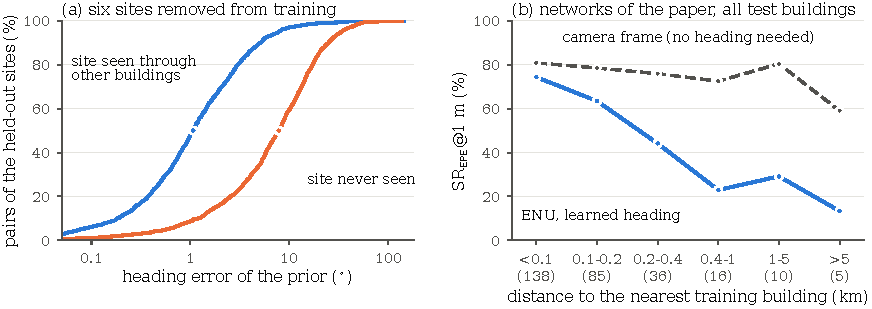
\includegraphics[width=0.92\textwidth]{figures/fig_heading.pdf}
\caption{\textbf{The heading prior depends on having seen the site.} (a) Cumulative distribution of the heading error on the test pairs of six sites, for the raw-view network of the paper, which saw other buildings of these sites during training, and for the same network re-trained without them; dots mark the medians. (b) Endpoint success of the refined stage against the distance from the test building to the nearest training building, in ENU with the learned heading and in the camera frame; the number of test buildings is given in parentheses.}
\label{fig:heading}
\end{figure*}

\begin{table}[t]
\centering
\caption{\textbf{Heading prior on sites that were never seen.} Raw-view heading network re-trained after removing every building of six sites from its training set; estimates of the refined stage rotated into ENU with the fused heading of this network. Heading error in degrees.}
\label{tab:heading_site}
\footnotesize
\setlength{\tabcolsep}{3pt}
\resizebox{\columnwidth}{!}{%
\begin{tabular}{@{}lccccc@{}}
\toprule
& \multicolumn{3}{c}{Heading error} & EPE med. & \SRe, ENU \\
\cmidrule(lr){2-4}
Heading network & mean & med. & $>10^\circ$ (\%) & (m) & (\%) \\
\midrule
\multicolumn{6}{@{}l}{\emph{Held-out sites} (84 test buildings, 1{,}852 pairs; camera frame: 78.4\% \SRe)}\\
\quad paper network & 2.4 \ci{1.7}{3.2} & 1.1 & 3.0 & 0.73 & 67.5 \ci{63.3}{71.9} \\
\quad re-trained without the six sites & 11.2 \ci{9.4}{13.1} & 7.8 & 40.6 & 1.78 & 27.4 \ci{22.4}{32.5} \\
\midrule\multicolumn{6}{@{}l}{\emph{Other sites} (206 test buildings, 4{,}512 pairs; camera frame: 78.8\% \SRe)}\\
\quad paper network & 7.1 \ci{4.9}{10.1} & 2.0 & 14.2 & 0.89 & 55.4 \ci{51.3}{58.9} \\
\quad re-trained without the six sites & 6.5 \ci{4.9}{8.5} & 2.4 & 16.6 & 0.96 & 51.8 \ci{47.9}{55.3} \\
\bottomrule
\end{tabular}}
\end{table}


\subsection{Dependence on the training sites}
\label{sec:headsite}

The test buildings are held out, but their surroundings are not. The buildings of PairUAV are grouped in campuses, and the median test building stands \hdDistMedian\,m from a training building (90th percentile \hdDistPNinety\,m), less than the width of the ground footprint of one image. \Cref{fig:heading}(b) shows the consequence. For the \hdDistAN{} test buildings within 100\,m of a training building the median heading error is $\hdDistAMed^\circ$ and the ENU success \hdDistAEnu\%; between 0.4 and 1\,km they are $\hdDistDMed^\circ$ and \hdDistDEnu\%; for the \hdDistFN{} buildings farther than 5\,km, $\hdDistFMed^\circ$ and \hdDistFEnu\%. The camera-frame success stays between \hdDistDCam\% and \hdDistACam\% up to 5\,km; its lower value for the last \hdDistFN{} buildings (\hdDistFCam\%) has an interval of \ci{\sgZeroSReLo}{\sgZeroSReHi} and is not significant. Over all test buildings the camera-frame success is unrelated to the number of training buildings of the site (Spearman \sgRho).

To measure the prior on sites that were never seen, we re-train the raw-view network after removing all \hdSdRemoved{} training buildings of \hdSdSites{} sites, which contain \hdSdBuildings{} test buildings (\cref{tab:heading_site}, \cref{fig:heading}(a)). On these sites the median heading error rises from $\hdSdSeenMed^\circ$ to $\hdSdUnseenMed^\circ$ and the ENU endpoint success falls from \hdSdSeenSRe\% to \hdSdUnseenSRe\%, a paired difference of \hdSdDelta{} points \ci{\hdSdDeltaLo}{\hdSdDeltaHi}; the camera-frame success on the same pairs is \hdSdCamSRe\%. On the other sites the re-trained network changes the success by \hdSdOtherDelta{} points \ci{\hdSdOtherDeltaLo}{\hdSdOtherDeltaHi}, which is the effect of the smaller training set alone. On an unseen site the error is close to one constant offset for the whole site, between $\hdSdOffMin^\circ$ and $\hdSdOffMax^\circ$ for the six sites, with a resultant length of the signed errors of \hdSdResLo{} to \hdSdResHi. Three limitations apply: only the raw-view network was re-trained, so both rows of \cref{tab:heading_site} use one network instead of two; there is one split and one seed; and a control with the same number of training buildings removed elsewhere was not trained to convergence.

The ENU results of Tables~2 and~3 therefore hold for test buildings that stand next to training buildings. They should not be read as results on unseen scenes, and the statement of the abstract on this point is corrected in \cref{sec:corrections}.

\begin{table}[t]
\centering
\caption{\textbf{What the heading prior reads.} Error of the heading predicted from one image (both networks) after an image operation, on 2{,}000 test images (degrees). $^\dagger$raw-view network only; a zoom of 3.6 corresponds to the flight height of the real photographs.}
\label{tab:heading_sens}
\footnotesize
\setlength{\tabcolsep}{3pt}
\resizebox{\columnwidth}{!}{%
\begin{tabular}{@{}lccc@{}}
\toprule
Operation on the image & Mean & Median & $>45^\circ$ (\%) \\
\midrule
None & 6.5 & 1.7 & 3 \\
\midrule Brightness $\times0.6$, $\times1.4$ & 6.9, 7.1 & 1.8, 1.9 & 3, 3 \\
Contrast $\times0.6$, $\times1.4$ & 7.3, 7.0 & 1.9, 2.0 & 3, 3 \\
Gamma 0.6, 1.6 & 8.8, 8.8 & 3.3, 2.7 & 3, 4 \\
Shadows lifted & 7.7 & 2.0 & 3 \\
Tiles of 64, 32 px shuffled & 10.0, 16.5 & 4.0, 7.6 & 4, 8 \\
\midrule Blur, $\sigma{=}1$, 2 px & 9.0, 21.7 & 3.1, 9.8 & 4, 14 \\
JPEG, quality 20 & 26.5 & 12.2 & 18 \\
Grey levels only & 43.5 & 35.7 & 39 \\
Hue rotated by $90^\circ$, $180^\circ$ & 39.1, 88.6 & 19.6, 89.6 & 29, 69 \\
Luminance inverted, colour kept & 91.9 & 93.5 & 72 \\
Negative image & 135.4 & 156.0 & 91 \\
\midrule Centre zoom $\times1.5$, $\times2$, $\times3.6^\dagger$ & 10.8, 16.0, 33.7 & 4.0, 6.4, 16.7 & 4, 8, 23 \\
\bottomrule
\end{tabular}}
\end{table}


\subsection{What the prior reads}
\label{sec:headsens}

\Cref{tab:heading_sens} applies image operations to \hdSensN{} test images. Global changes of brightness, contrast and gamma, lifting the shadows, and even shuffling tiles of 64 pixels leave the prediction almost unchanged: the cue is local, not the layout of the scene. Removing the colour (median error $\hdSensGray^\circ$), rotating the hue ($\hdSensHue^\circ$ for $180^\circ$), strong compression ($\hdSensJpeg^\circ$) and blur degrade it severely, and on the negative image \hdSensNegFlip\% of the predictions turn by $180^\circ$. A change of scale by 3.6, that of the real photographs, gives a median error of $\hdSensZoom^\circ$. For the \hdSouthN{} test buildings of the southern hemisphere the median error is $\hdSouthErr^\circ$. These observations are consistent with a cue tied to the direction of the illumination, such as the shadows, whose relation to north is fixed for the imagery of a site and reverses in the southern hemisphere. We have not verified this interpretation directly: the dataset has one rendering per site, so the illumination cannot be varied in a controlled way. Whatever the cue, it is a property of the imagery from which PairUAV is rendered and not of the scene.

On the real photographs the prior does not transfer: the median error is $\hdRealOneMed^\circ$ from one image and $\hdRealFusedMed^\circ$ after fusion, where chance is $90^\circ$, and the ENU endpoint success is \hdRealEnuSRe\% against \hdRealCamSRe\% in the camera frame (\cref{sec:real}). The failure is at least detectable: the median concentration predicted by the raw-view network falls from \hdRenderKappa{} on the rendered test images to \hdRealKappa{} on the photographs.

\begin{table}[t]
\centering
\caption{\textbf{Baselines of Table~2 re-trained with the horizontal target in the camera frame} (same recipes; 6{,}364 test pairs). Hor.: mean absolute error of the two horizontal components; Corr.: correlation between predicted and true horizontal components, averaged over the two. A number in parentheses: recipes repeated with that many seeds, mean reported. $\pi_{0.5}$ and $\pi_0$-FAST were not re-trained.}
\label{tab:camframe}
\footnotesize
\setlength{\tabcolsep}{2.5pt}
\resizebox{\columnwidth}{!}{%
\begin{tabular}{@{}lcccccccccc@{}}
\toprule
& \multicolumn{2}{c}{$d$ (m)} & \multicolumn{2}{c}{\SRd{} (\%)} & \multicolumn{2}{c}{Hor. (m)} & \multicolumn{2}{c}{Corr.} & \multicolumn{2}{c}{EPE med. (m)} \\
\cmidrule(lr){2-3}\cmidrule(lr){4-5}\cmidrule(lr){6-7}\cmidrule(lr){8-9}\cmidrule(lr){10-11}
Training target & ENU & cam. & ENU & cam. & ENU & cam. & ENU & cam. & ENU & cam. \\
\midrule
ViNT & 18.91 & 18.40 & 0.3 & 0.2 & 7.46 & 7.26 & $-0.01$ & $+0.02$ & 20.0 & 20.1 \\
NoMaD & 7.14 & 7.08 & 8.6 & 8.6 & 9.62 & 9.57 & 0.00 & $+0.01$ & 25.2 & 25.1 \\
DINO-WM (2) & 10.33 & 10.27 & 6.1 & 6.1 & 8.94 & 8.87 & $-0.01$ & $-0.01$ & 23.6 & 23.7 \\
Visual Foresight & 10.30 & 10.28 & 5.7 & 5.7 & 8.73 & 8.54 & $-0.01$ & $+0.01$ & 23.0 & 22.9 \\
DINOv3 ViT-7B (5) & 12.86 & 13.05 & 3.1 & 3.0 & 7.83 & 7.57 & $+0.01$ & $+0.02$ & 19.2 & 19.1 \\
Sample4Geo (5) & 11.00 & 10.30 & 5.1 & 5.7 & 8.29 & 8.58 & $+0.01$ & $+0.01$ & 21.0 & 21.7 \\
\midrule
Regression on MASt3R statistics & 5.40 & 3.15 & 9.9 & 21.5 & 7.44 & 3.68 & $+0.07$ & $+0.83$ & 12.2 & 6.1 \\
\midrule
No motion & 20.32 & 20.32 & 0.0 & 0.0 & 7.45 & 7.26 & -- & -- & 20.2 & 20.2 \\
\bottomrule
\end{tabular}}
\end{table}


\subsection{Do the baselines fail because of the frame?}
\label{sec:camframe}

One review suspects that the baselines of Table~2 fail mainly because they must regress $\Delta x$ and $\Delta y$ in ENU. We re-trained six of the eight with the horizontal target in the camera frame, with otherwise the recipes of Table~2 (\cref{sec:baselines}); $\pi_{0.5}$ and $\pi_0$-FAST could not be re-trained on the shared GPU. \Cref{tab:camframe} shows no effect. In both frames the horizontal error of every re-trained baseline is at or above that of predicting no motion (\cfZeroCamHor\,m), the correlation between its predicted and the true horizontal displacement is at most \cfMaxCamCorr, its endpoint success at 1\,m is at most \cfMaxCamSRe\%, and its \SRd{} (at most \cfMaxCamSRd\%) is at the level of a constant distance equal to the training median (\cfConstSRd\%). These models do not perceive the displacement at all; the frame of the target is not what limits them. Three diagnostics support this. ViNT and NoMaD receive inputs of $85{\times}64$ and $96{\times}96$ pixels, in which one metre on the ground is half a pixel. Heads trained to convergence on the frozen DINOv3 and Sample4Geo descriptors stay at the level of no motion in both frames. For the two world models the planning cost changes by less than 0.1\% when the horizontal displacement of the action is exchanged with that of another pair.

The concern is nevertheless justified for a model that does perceive the displacement. The regression on pooled MASt3R statistics, which is the prior branch of DreamNav, improves from \cfMlpEnuD\,m to \cfMlpCamD\,m of range error and from \cfMlpEnuSRd\% to \cfMlpCamSRd\% \SRd{} when its target is expressed in the camera frame, and the correlation of its horizontal prediction with the truth from \cfMlpEnuCorr{} to \cfMlpCamCorr. For this reason all results of this document are given in the camera frame, and \cref{tab:main_metrics} gives both frames for our method.

\section{How far does a ground-plane warp carry?}
\label{sec:planarity}

Two reviewers questioned the plane-induced warp of Eq.~(5): the scenes of PairUAV contain buildings, the motivation of the paper mentions windows and balconies, and no result was broken down by scene structure. \Cref{sec:imag} specifies how $\mathbf{n}$ and $h$ are obtained. Here we measure how planar the scenes are and how the accuracy varies with their relief.

\noindent\textbf{Measuring relief.} For each test pair we triangulate the matches of the imagination pass with the ground-truth relative pose. The ground truth is used only to describe the scene; no method sees it. As in \cref{sec:cands}, $b_i$ is the depth of a point below the source camera along gravity. We take the 85th percentile $g$ of the $b_i$ as the ground level, $S=g-P_5(b)$ as the height of the tallest matched structures, and call $S/g$ the \emph{relief} of the pair: the building height over the flight height that the reviewers asked for. Over the \plN{} pairs with at least 200 triangulated matches, $g$ agrees with the height of the camera above the terrain model of the renderer (correlation \plTerrCorr, median absolute difference \plTerrDiff\,m).

\noindent\textbf{The scenes are not planar, but their relief is small relative to the flight height.} The cameras fly \plGroundMed\,m above the ground (5th--95th percentile: \plGroundLo--\plGroundHi\,m; the distribution over the whole dataset is given in \cref{sec:dataset}), and the tilt covers $0^\circ$--$45^\circ$. The matched structures are $S{=}$\plStructMed\,m high in the median pair and \plStructHi\,m at the 95th percentile, which gives a relief of \plReliefMed\% (\plReliefLo--\plReliefHi\%). In the median pair only \plNearMed\% of the matched points lie within 2\,m of the ground, \plOffThreeMed\% are more than 3\,m above it and \plOffTenMed\% more than 10\,m: most matches are on roofs and vegetation, not on the ground. What the warp relies on is therefore not that points lie on the plane, but that the parallax of the points that do not is small: the first-order displacement $f\|\dpv\|S/g^2$ of the tallest structures is \plParallaxMed\,px in the median pair and \plParallaxHi\,px at the 95th percentile, at full resolution, for tiles of $1280{\times}720$\,px. The statement of Sec.~4.3 that the scene is ``mostly planar'' should be read in this sense. The ground itself is level: the slope of a plane fitted to the points within 2\,m of $g$ is \plSlopeMed$^\circ$ in the median pair (\plSlopeHi$^\circ$ at the 95th percentile).

\noindent\textbf{The plane is an alignment device, not the pose model.} As stated in \cref{sec:imag}, the homography only pre-aligns the two images. The refined pose comes from the epipolar constraints of the new matches, which hold for points at any height. Points on roofs are not outliers of the refinement; they are the matches that carry the parallax from which the translation is observed. \Cref{fig:imagination} shows both situations.

\begin{figure*}[t]
\centering
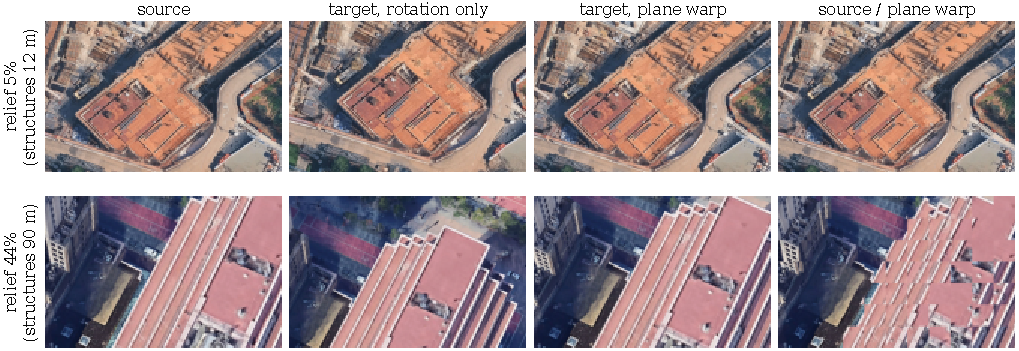
\includegraphics[width=\textwidth]{figures/fig_imagination.pdf}
\caption{\textbf{What the plane-induced warp aligns.} Two test pairs with a baseline of about \fgLowDist\,m and an altitude change of \fgLowDz\,m, warped with the coarse pose (no ground truth). Top: \fgLowRelief\% relief; the rotation alone leaves the change of scale and position, the plane-induced warp aligns the views to \fgLowRes\,px (median over the matches). Bottom: one of the tallest scenes of the test set (\fgHighRelief\% relief, a \fgHighStruct\,m tower); the street is aligned, the roof is displaced by parallax (\fgHighRes\,px), and the tile-wise matcher still returns \fgHighInl{} inliers, which the epipolar re-estimation uses. Last column: checkerboard of the source and the plane-warped target.}
\label{fig:imagination}
\end{figure*}

\begin{table}[t]
\centering
\caption{\textbf{Accuracy against scene relief} (6{,}193 test pairs). Relief: height of the tallest matched structures over the flight height. $S$: that height in metres (median). Res.: median displacement between the imagined and the real view. I / II: coarse / refined stage, camera frame.}
\label{tab:planarity}
\footnotesize
\setlength{\tabcolsep}{2.6pt}
\begin{tabular}{@{}lrrrcccccc@{}}
\toprule
& & $S$ & Res. & \multicolumn{2}{c}{\SRd@1\,m} & \multicolumn{2}{c}{\SRe@1\,m} & \multicolumn{2}{c}{$\dpsi$ MAE} \\
Relief & Pairs & (m) & (px) & I & II & I & II & I & II \\
\midrule
$<$2\% & 34 & 4 & 27.1 & 29.4 & 52.9 & 11.8 & 26.5 & 1.74 & 1.18 \\
2-5\% & 447 & 9 & 12.4 & 51.0 & 71.1 & 28.0 & 58.4 & 0.93 & 0.45 \\
5-10\% & 3683 & 17 & 7.1 & 75.2 & 86.3 & 61.9 & 82.7 & 0.37 & 0.12 \\
10-15\% & 1426 & 25 & 7.3 & 79.0 & 85.1 & 69.3 & 82.5 & 0.25 & 0.09 \\
15-20\% & 330 & 38 & 7.8 & 77.3 & 83.9 & 67.0 & 80.0 & 0.27 & 0.12 \\
20-30\% & 191 & 51 & 8.6 & 78.5 & 87.4 & 70.2 & 84.8 & 0.29 & 0.07 \\
$\geq$30\% & 82 & 79 & 11.6 & 73.2 & 79.3 & 63.4 & 74.4 & 0.22 & 0.15 \\
\bottomrule
\end{tabular}
\end{table}

\begin{table}[t]
\centering
\caption{\textbf{Accuracy against the larger tilt of the pair} (top), \textbf{the height of the source camera above the ground} (middle) \textbf{and the baseline-to-height ratio} (bottom). Same pairs and columns as \cref{tab:planarity}.}
\label{tab:planarity_tilt}
\footnotesize
\setlength{\tabcolsep}{4pt}
\begin{tabular}{@{}lrrcccc@{}}
\toprule
& & Res. & \multicolumn{2}{c}{\SRd@1\,m} & \multicolumn{2}{c}{\SRe@1\,m} \\
Bin & Pairs & (px) & I & II & I & II \\
\midrule
0-15$^\circ$ & 798 & 5.7 & 92.2 & 93.4 & 89.2 & 92.5 \\
15-25$^\circ$ & 1397 & 6.3 & 83.2 & 88.7 & 75.0 & 86.5 \\
25-35$^\circ$ & 1924 & 7.6 & 76.5 & 84.6 & 62.0 & 80.9 \\
35-45$^\circ$ & 2074 & 10.0 & 59.2 & 78.4 & 41.0 & 71.2 \\
\midrule
190-210\,m & 1231 & 7.8 & 75.1 & 81.7 & 62.4 & 77.7 \\
210-230\,m & 3114 & 7.3 & 74.1 & 86.9 & 61.8 & 82.7 \\
230-250\,m & 1773 & 7.1 & 75.6 & 84.9 & 61.8 & 80.5 \\
$\geq$250\,m & 62 & 8.6 & 43.5 & 37.1 & 22.6 & 30.6 \\
\midrule
$<$3\% & 113 & 14.0 & 67.3 & 80.5 & 36.3 & 63.7 \\
3-6\% & 1016 & 7.6 & 71.8 & 86.6 & 56.6 & 80.7 \\
6-9\% & 1898 & 7.8 & 70.5 & 82.1 & 57.6 & 77.9 \\
9-12\% & 1799 & 7.0 & 75.7 & 83.9 & 63.5 & 80.5 \\
$\geq$12\% & 1367 & 7.2 & 80.0 & 87.7 & 69.6 & 84.9 \\
\bottomrule
\end{tabular}
\end{table}


\noindent\textbf{Accuracy against relief.} \Cref{tab:planarity} bins the test pairs by relief. The refinement improves every bin. Its gain in endpoint success is largest on the flattest scenes, +\plGainA{} points \ci{\plGainALo}{\plGainAHi} below 5\% relief, and remains +\plGainC{} \ci{\plGainCLo}{\plGainCHi} between 10\% and 20\% and +\plGainD{} \ci{\plGainDLo}{\plGainDHi} above 20\%. Between 5\% and 30\% of relief, the refined success is flat (\SRd{} between \plMidSRdLo\% and \plMidSRdHi\%), and the displacement between the imagined and the real view stays at about \plResMid\,px. This displacement is mostly the parallax of the matched structures, not the error of the coarse pose: when the warp is computed from the true pose instead (\rgOracleN{} pairs, \cref{tab:raw_geometry}), its median only falls from \rgOursSubRes\,px to \rgOracleRes\,px. It does not follow the relief $S/g$ (Spearman \plSpearRes), because it reflects the typical height of the matched points above the ground rather than the tallest structure. Two regimes are harder. (i) The \plFlatN{} pairs below 5\% of relief are the hardest for \emph{both} stages (coarse \SRd{} \plFlatSiSRd\%, refined \plFlatSiiSRd\%): a nearly planar scene is the ill-conditioned case of two-view geometry discussed in Sec.~4.2, the coarse pose is less accurate there (residual of \plFlatRes\,px), and this is precisely where the plane-induced warp is most faithful and brings its largest gain. (ii) Above 30\% of relief (\plTallN{} pairs) the refined \SRd{} is \plTallSiiSRd\%, a few points below the middle bins. We therefore find no evidence that relief, within the range present in PairUAV, is what limits the refinement.

\noindent\textbf{Tilt, flight height and baseline.} \Cref{tab:planarity_tilt} shows stronger effects than relief. The accuracy decreases with the tilt of the more oblique camera: from \plTiltLoSiiSRd\% to \plTiltHiSiiSRd\% in \SRd{} after refinement, the coarse stage dropping from \plTiltLoSiSRd\% to \plTiltHiSiSRd\%; oblique pairs are the ones on which the refinement helps most. And the \plHighN{} pairs whose source camera is more than 250\,m above the ground are poorly handled by both stages (\plHighSiSRd\% and \plHighSiiSRd\%): the flight-height cue and the bounds on $h$ (\cref{sec:cands,sec:imag}) are calibrated on the training distribution, and DreamNav should not be expected to work at a flight height that differs markedly from it without the height being provided, as it is for the real photographs of \cref{sec:real}. Finally, the shortest baselines, below 3\% of the flight height (\plShortN{} pairs), are the hardest for the coarse stage in endpoint terms (\plShortSiSRe\%) and gain the most from the refinement (\plShortSiiSRe\%).

\noindent\textbf{Scope.} PairUAV views are taken from about 200 to 240\,m above the ground with tilts up to $45^\circ$. The windows and balconies of the introduction motivate why metre-level accuracy is needed at the end of an approach; they do not describe the viewing geometry of the benchmark, and Fig.~1 should not be read as a claim about close-range flight along a facade. In that regime a vertical surface dominates the view, the ground may not be visible, and a ground-plane warp would not align the two images. The closed form of Eq.~(5) would still apply to the facade plane, with a different $\mathbf{n}$ and $h$, but we have not evaluated it and make no claim about it. The real photographs of Sec.~5.3, taken 60\,m above a village, have about 3.7 times the relative relief of PairUAV for the same structures; the refinement still improves on them (\cref{sec:real}).

\section{Closed-loop experiment}
\label{sec:closedloop}

The reviews raise four points about Sec.~5.4: Table~5 reports one draw of the actuation noise on 160 episodes, without uncertainty; the abstract mixes the internal refinement with physical steps; the one-step success of Table~5 (38.8\%) is far below the 83.3\% of Table~2; and there is no classical visual-servoing baseline, which limits what the experiment shows. While preparing the answers we found that the row ``Ours (Stage~II)'' of Table~5 contains a component that the main paper does not describe. We start with it, because it changes the reading of the table.

\subsection{What the rows of Table~5 are}
\label{sec:tablefive}

\noindent\textbf{Simulator.} Each of the \clSites{} held-out sites is reconstructed by 3-D Gaussian splatting~\cite{kerbl20233d,ye2025gsplat} from 135 of its 150 posed images; the 15 other images are never seen by the reconstruction (their rendering has a PSNR of 23.9\,dB on average). An episode takes one of these held-out \emph{real} photographs as the goal and the pose of another camera of the site as the start (10 goals per site, 2 starts per goal, \clEpisodes{} episodes). At every step the estimator receives a view \emph{rendered} at the current pose and the goal photograph, and outputs a displacement in the levelled frame of the current camera, which is applied to the pose with noise: 3\% of the commanded move plus 5\,cm per axis, $0.2^\circ$ in heading and $0.1^\circ$ in tilt. There are no dynamics, no flight controller, no wind and no obstacles; the absolute heading is not used.

\noindent\textbf{Three estimators, not two.} ``Ours (Stage~I)'' is the coarse stage. ``Ours (Stage~II)'' is the refined stage of Sec.~4.3 \emph{plus} the short-range ground-plane solver of \cref{sec:shortrange}, which replaces the fused translation whenever the estimated remaining distance is below 5\,m and at least 200 matches support it. The main paper does not mention this solver, although it provides the translation in \clPlaneSteps\% of all steps of this row (\clPlaneFirst\% of the first steps, \clPlaneSecond\% of the second and \clPlaneThird\% of the third) and acts at least once in \clPlaneFlights\% of the episodes. \Cref{tab:closedloop} therefore adds the missing row, the refined stage as described in the paper.

\begin{table*}[t]
\centering
\caption{\textbf{Closed loop of Table~5 with the three estimators separated} (160 episodes on 8 held-out sites, at most 5 steps; SR: mean\,$\pm$\,standard deviation over 4 draws of the actuation noise, the first being the draw of Table~5; other columns: mean). The run stops when the estimated remaining distance is below $\tau$. SR: final position within 1\,m; Err.: median final position error; brackets: 95\,\% interval of a bootstrap over episodes.}
\label{tab:closedloop}
\footnotesize
\setlength{\tabcolsep}{4pt}
\resizebox{\textwidth}{!}{%
\begin{tabular}{@{}lcccccccccc@{}}
\toprule
& One step & \multicolumn{2}{c}{$\tau{=}0.5$\,m} & \multicolumn{3}{c}{$\tau{=}1$\,m} & \multicolumn{2}{c}{$\tau{=}1.5$\,m} & \multicolumn{2}{c}{$\tau{=}2$\,m} \\
\cmidrule(lr){3-4}\cmidrule(lr){5-7}\cmidrule(lr){8-9}\cmidrule(lr){10-11}
Estimator & SR (\%) & Steps & SR (\%) & Steps & Err. (m) & SR (\%) & Steps & SR (\%) & Steps & SR (\%) \\
\midrule
Coarse (Table~5, ``Stage~I'') & 35.5\,$\pm$\,1.7 & 4.9 & 25.6\,$\pm$\,3.3 & 3.9 & 1.01 & 50.3\,$\pm$\,5.9 \ci{45.9}{55.2} & 2.9 & 68.6\,$\pm$\,1.8 & 2.3 & 66.1\,$\pm$\,3.2 \\
Coarse + refined & 41.1\,$\pm$\,1.2 & 4.8 & 24.5\,$\pm$\,2.1 & 3.8 & 1.01 & 49.8\,$\pm$\,4.5 \ci{45.3}{54.5} & 2.7 & 70.5\,$\pm$\,2.1 & 2.1 & 68.6\,$\pm$\,4.0 \\
Coarse + refined + short-range (Table~5, ``Stage~II'') & 38.4\,$\pm$\,2.3 & 3.7 & 64.5\,$\pm$\,2.1 & 2.3 & 0.62 & 80.3\,$\pm$\,4.6 \ci{76.9}{83.9} & 1.8 & 71.6\,$\pm$\,3.0 & 1.6 & 63.6\,$\pm$\,4.9 \\
\bottomrule
\end{tabular}}
\end{table*}

\begin{table}[t]
\centering
\caption{\textbf{Without a stopping rule}: share of the episodes of \cref{tab:closedloop} within 1\,m of the goal after each step (\%, mean over the draws), and median position error after the fifth step.}
\label{tab:fixedsteps}
\footnotesize
\setlength{\tabcolsep}{4pt}
\resizebox{\columnwidth}{!}{%
\begin{tabular}{@{}lcccccc@{}}
\toprule
& \multicolumn{5}{c}{SR after step} & Err. \\
\cmidrule(lr){2-6}
Estimator & 1 & 2 & 3 & 4 & 5 & (m) \\
\midrule
Coarse & 35.5 & 39.5 & 28.6 & 23.6 & 22.0 & 1.58 \\
Coarse + refined & 41.1 & 34.2 & 16.9 & 19.2 & 17.7 & 1.68 \\
Coarse + refined + short-range & 38.4 & 66.9 & 59.1 & 49.5 & 53.3 & 0.93 \\
\bottomrule
\end{tabular}}
\end{table}


\subsection{Uncertainty, and where the gain comes from}
\label{sec:cluncertainty}

\Cref{tab:closedloop} repeats the experiment with the actuation noise re-drawn (\clDrawsText; the estimator itself is deterministic) and gives bootstrap intervals over episodes.\clSpreadText{} With the stopping threshold $\tau{=}1$\,m the coarse stage reaches \clSiSR\% on average, the refined stage \clSiiPlainSR\% and the refined stage with the short-range solver \clSiiSR\%; the draw of Table~5 was a favourable one for all three (56.9\%, 55.6\% and 81.9\%). On the same episodes the differences are
\begin{itemize}[leftmargin=*,itemsep=1pt,topsep=2pt]
\item refined $-$ coarse: \clDrefine{} points \ci{\clDrefineLo}{\clDrefineHi};
\item short-range solver on top of the refined stage: \clDplane{} points \ci{\clDplaneLo}{\clDplaneHi};
\item Table~5, ``Stage~II'' $-$ ``Stage~I'': \clDfull{} points \ci{\clDfullLo}{\clDfullHi} (bootstrap over sites: \ci{\clDfullSiteLo}{\clDfullSiteHi}).
\end{itemize}
The difference between the two rows of Table~5 is therefore real, but it is the contribution of the short-range solver. \emph{The imagination-refined stage by itself does not improve the closed loop over the coarse stage.} The sentence of Sec.~5.4 that attributes the improvement to the refinement, and the corresponding sentence of the abstract, are not supported (\cref{sec:corrections}).

The reason is visible in \cref{tab:fixedsteps}. Without a stopping rule, the success of the coarse and of the refined stage \emph{decreases} after the second step (\clSiFixTwo\% to \clSiFixFive\%, and \clSiiPlainFixTwo\% to \clSiiPlainFixFive\%): within a few metres of the goal both estimators are inaccurate and move the camera away again. The released pairs contain almost no such configuration: \dsShortFive\% of them have a baseline below 5\,m, and \dsFusionShortFive{} of the \dsFusionRows{} pairs on which the fusion is fitted, of which \dsFusionShortTwo{} are below 2\,m (\cref{sec:dataset}). The learned fusion therefore extrapolates near the goal, and the essential matrix loses the translation direction as the baseline vanishes. The short-range solver addresses exactly this regime (\clSiiFixTwo\% after two steps), although its success also decreases when the loop continues (\clSiiFixFive\% after five). The stopping rule is thus an essential part of the result: the success at $\tau{=}1$\,m is the highest of the four thresholds of Table~5 (\clSiiSRhalf\% at 0.5\,m, \clSiiSRtwo\% at 2\,m), and $\tau$ was not selected on separate episodes.

\subsection{Internal refinement and physical steps}
\label{sec:internalphysical}

The 2.2 steps of the abstract are physical steps: each one is a commanded move followed by a new observation rendered at the new pose, and each estimate runs the refinement once. Nothing is iterated inside the estimator. The sentences ``Iterating the refinement 2.2 times [...]'' and ``the loop closes inside the estimator rather than in the air'' describe a different mechanism from the one that was evaluated and are withdrawn. When the refinement \emph{is} iterated on a fixed pair, without motion, the endpoint success changes by \itThreeASRe{} to \itThreeBSRe{} points after three rounds (\cref{sec:iteration}); the gain of the closed loop comes from new observations taken closer to the goal.

\begin{table}[t]
\centering
\caption{\textbf{From Table~2 to the one-step column of Table~5.} Success of one estimate on the test pairs, on the start/goal pairs of the simulated episodes, and after the commanded move is executed (position within 1\,m of the goal; with noise: expectation over 2{,}000 draws and the range that contains 95\,\% of single draws). Camera frame.}
\label{tab:onestep}
\footnotesize
\setlength{\tabcolsep}{3pt}
\resizebox{\columnwidth}{!}{%
\begin{tabular}{@{}lrcccc@{}}
\toprule
& & \multicolumn{2}{c}{Coarse} & \multicolumn{2}{c}{Refined} \\
\cmidrule(lr){3-4}\cmidrule(lr){5-6}
& Pairs & \SRd & \SRe & \SRd & \SRe \\
\midrule
Test pairs of Table~2 & 6{,}364 & 73.1 & 59.9 & 83.3 & 78.7 \ci{77.0}{80.2} \\
\quad of the simulator sites & 165 & 72.1 & 56.4 & 81.8 & 77.6 \\
Episode pairs, real start photograph & 160 & 54.4 & 48.1 & 64.4 & 60.6 \ci{53.7}{68.1} \\
Episode pairs, rendered start view & 160 & 51.9 & 45.0 & 56.2 & 48.1 \ci{40.6}{55.6} \\
\midrule
After the move, no actuation noise & 160 & -- & 43.8 & -- & 47.5 \ci{40.0}{55.0} \\
After the move, with actuation noise & 160 & -- & 35.4 & -- & 39.5 \ci{35.0}{44.4} \\
\quad the single draw of Table~5 & 160 & -- & 37.5 & -- & 41.9 \\
\bottomrule
\end{tabular}}
\end{table}


\subsection{From Table~2 to the one-step column of Table~5}
\label{sec:onestep}

One review asks why a single step succeeds in 38.8\% of the episodes when 83.3\% of the test pairs are within 1\,m. \Cref{tab:onestep} follows the estimate from one setting to the other.

\noindent\textbf{Definition.} Table~2 counts the range error; Table~5 counts the distance between the reached and the goal position. On the test pairs the corresponding endpoint success is \SiiCamSRe\% (\cref{sec:whichdef}).

\noindent\textbf{Pair distribution.} The test pairs of the simulator sites are as easy as the others (\ogSiteSRd\% / \ogSiteSRe\% on \ogSiteN{} pairs). The episodes, however, pair a goal with an arbitrary camera of the site: they are not screened for overlap, and \ogOutside\% of them lie outside the ranges of horizontal displacement of the released pairs. On the real start photographs of the episodes the refined stage succeeds on \ogRealSRd\% / \ogRealSRe\% (\ogRealInSRe\% of endpoint success inside the released ranges, \ogRealOutSRe\% outside). This step accounts for about 18 of the 39 points and is the effect of the pair selection that the reviews ask about (\cref{sec:unscreened}).

\noindent\textbf{Rendering.} When the start view is rendered by the simulator instead of photographed, the endpoint success falls to \ogRendSRe\%. The estimator is sensitive to the rendering gap of the simulator, and this affects every later observation of an episode. The closed-loop numbers are therefore conservative with respect to real images in this respect, and say nothing about the opposite direction, a real aircraft.

\noindent\textbf{Execution.} Executing the commanded displacement without noise leaves \ogNoNoise\% of the episodes within 1\,m. The actuation noise alone moves the camera by \ogNoiseDisp\,m in the median at these distances; in expectation over 2{,}000 draws the success is \ogNoise\%, and 95\% of single draws fall in \ci{\ogNoiseLo}{\ogNoiseHi}. The 38.8\% of Table~5 is one such draw, for the row with the short-range solver; the refined stage alone drew 41.9\%.

\begin{table}[t]
\centering
\caption{\textbf{Classical visual servoing in the simulator of Table~5} (same 160 episodes and actuation noise, one noise draw). SR: true position within 1\,m of the goal, after 1, 2, 5 steps and at the end of the step budget $T$. ``$>$50\,m'': episodes that move more than 50\,m away from the goal during the flight. Last two columns: steps flown and SR when the policy stops once its own estimate of the remaining distance is below 1\,m.}
\label{tab:servo}
\footnotesize
\setlength{\tabcolsep}{2.6pt}
\resizebox{\columnwidth}{!}{%
\begin{tabular}{@{}lccccccccc@{}}
\toprule
& & \multicolumn{4}{c}{SR (\%) after} & Err. & $>$50\,m & \multicolumn{2}{c}{Stop at 1\,m} \\
Policy & $T$ & 1 & 2 & 5 & $T$ & (m) & (\%) & steps & SR \\
\midrule
IBVS, gain 0.5 & 20 & 0.0 & 0.0 & 6.2 & 91.2 & 0.20 & 55.6 & 10.2 & 83.8 \\
IBVS, gain 1 & 5 & 0.0 & 5.6 & 68.8 & 68.8 & 0.26 & 49.4 & 4.1 & 67.5 \\
Direct geometric servo & 5 & 22.5 & 41.2 & 67.5 & 67.5 & 0.65 & 5.0 & 2.7 & 62.5 \\
\midrule
Ours, coarse stage & 5 & 37.5 & 42.5 & 25.0 & 25.0 & 1.53 & 0.0 & 3.8 & 56.9 \\
Ours, refined stage & 5 & 41.9 & 31.9 & 18.8 & 18.8 & 1.75 & 0.0 & 3.7 & 55.6 \\
Ours, refined + short-range & 5 & 38.8 & 73.1 & 56.9 & 56.9 & 0.87 & 0.0 & 2.2 & 81.9 \\
\bottomrule
\end{tabular}}
\end{table}


\subsection{Classical visual servoing}
\label{sec:servo}

\Cref{tab:servo} adds three classical controllers in the same simulator, with the same episodes and noise. All three use the matches of our first pass, because off-the-shelf matching leaves half of the episodes without any feature (\cref{sec:georesults}), and take the depth of the features from the flight height. \emph{IBVS} is image-based visual servoing on point features~\cite{chaumette2006visual} with the point interaction matrix and robust weights, with a gain of 0.5 over 20 steps or a gain of 1 over 5 steps. The \emph{direct geometric servo} executes at each step the pose of the essential matrix with the flight-height scale, with no learned component.

IBVS with the small gain and 20 steps ends within 1\,m of the goal in \svIbvsFinal\% of the episodes, more than any row of Table~5, with a median final error of \svIbvsMed\,m. It needs many steps (\svIbvsStopSteps{} with the stopping rule at 1\,m, for \svIbvsStopSR\%), and its trajectories are not acceptable as they are: in \svIbvsExc\% of the episodes the camera moves more than 50\,m away from the goal before converging; we attribute this to a control law that is only locally valid and to the few, poorly distributed features of the first steps. The direct geometric servo reaches \svGeoFinal\% after five steps. Our estimators are the most accurate at the first step (\svSiiAfterOne\% against \svGeoAfterOne\% and \svIbvsAfterOne\%) and never leave the neighbourhood of the goal, and with the short-range solver and the stopping rule they need \svSiipStopSteps{} steps for \svSiipStopSR\%.

\subsection{What the experiment supports}
\label{sec:clscope}

The closed-loop experiment shows that, in a simulator without dynamics, a few pose estimates with a stopping rule bring a camera from about 19\,m to within 1\,m of an image goal in about four fifths of the cases, provided that a solver adapted to short baselines takes over near the goal. It does not show that the imagination-refined stage improves the closed loop, that the method is preferable to classical servoing when more steps are allowed, or that the result transfers to an aircraft: flight dynamics, a controller, wind, obstacles and the difference between rendered and real views are outside the experiment. The statements of the abstract and of the conclusion on closed-loop navigation should be limited to this (\cref{sec:corrections}).

\section{Real photographs}
\label{sec:real}

The reviews note that the real-image experiment uses one dataset, reports medians without uncertainty, restricts the pairs, and includes no geometric baseline. This section gives the complete protocol, including one input that the main paper does not mention, and the results on all sampled pairs.

\noindent\textbf{Data.} The \rlImages{} photographs used come from flights of a DJI Phantom~4 RTK over a village, with the camera tilted by about \rlTilt$^\circ$ from the nadir and poses from RTK positioning and bundle adjustment. The photographs are undistorted and resampled to the calibration $K$ of PairUAV, and the labels are computed from the poses as for PairUAV. Among all ordered pairs whose cameras are at most 30\,m apart we sample 600: \rlNin{} with a baseline of at most \rlInMax\,m, which is the baseline-to-height range covered by PairUAV once scaled to this flight height (38\,m at 220\,m), and \rlNout{} beyond it. Table~4 of the main paper reports the first group, as its caption states; the second group was sampled at the same time and is reported here.

\noindent\textbf{Flight height.} DreamNav is not fine-tuned and sees no label of this dataset. It does, however, receive one number: the height above ground reported by the aircraft, 60\,m. The two DreamNav rows of Table~4 multiply the predicted displacement by $60/220.2$, the ratio of this height to the flight height at which the scale cues were calibrated (\cref{sec:cands}). The main paper omits this, and the baselines of Table~4 do not receive it. Without the flight height the output is too long by this factor and the median endpoint error is \rlNoHeightPos\,m (\cref{tab:real}); giving the same factor to the regression on MASt3R statistics lowers its median error to \rlMlpPos\,m. A height above ground is available on most UAVs (barometer, rangefinder or terrain model), but the claim of Sec.~5.3 should read ``zero-shot given the flight height''.

\begin{table*}[t]
\centering
\caption{\textbf{Real photographs: Table~4 re-scored with uncertainty}, in the camera frame of the first image unless noted, for the pairs within the baseline-to-height range of the training data (the pairs of Table~4) and beyond it. EPE: endpoint error; Table~4 reports its median as ``Pos.'' and \SRd{} as SR. Brackets: 95\% bootstrap intervals over source images. Angular errors of $\dth$ are mean / median. ``No flight height'': the output is not rescaled by the height reported by the aircraft.}
\label{tab:real}
\footnotesize
\setlength{\tabcolsep}{4pt}
\resizebox{\textwidth}{!}{%
\begin{tabular}{@{}lccccccccc@{}}
\toprule
& \multicolumn{2}{c}{EPE (m)} & \SRe@1\,m & \SRe@2\,m & \SRd@1\,m & \SRd@2\,m & $\dth$ error ($^\circ$) & $\dpsi$ MAE & Dir. med. \\
Method & median & mean & (\%) & (\%) & (\%) & (\%) & mean / med. & ($^\circ$) & ($^\circ$) \\
\midrule
\multicolumn{10}{@{}l}{\emph{Within the training range: 300 pairs, baselines 0.7--10.3\,m}}\\
ViNT & 7.75 \ci{7.55}{8.05} & 7.32 & 0.3 \ci{0.0}{1.0} & 3.3 & 3.7 & 8.0 & 71.34 / 60.29 & 14.53 & 90.6 \\
NoMaD & 21.21 \ci{20.31}{21.95} & 20.76 & 0.0 \ci{0.0}{0.0} & 0.0 & 0.3 & 2.3 & 86.01 / 81.75 & 17.86 & 89.5 \\
$\pi_0$-FAST & 25.93 \ci{25.46}{26.51} & 26.06 & 0.0 \ci{0.0}{0.0} & 0.0 & 0.0 & 0.0 & 94.26 / 113.22 & 4.43 & 91.8 \\
Constant (zero motion) & 7.84 \ci{7.45}{8.08} & 7.18 & 1.3 \ci{0.3}{2.7} & 3.7 & 1.3 & 3.7 & 83.71 / 89.34 & 0.45 & 90.0 \\
MASt3R-statistics MLP, flight height & 5.10 \ci{4.79}{5.30} & 5.28 & 1.7 \ci{0.3}{3.2} & 8.3 & 18.3 & 34.3 & 3.72 / 1.93 & 3.40 & 41.0 \\
\cmidrule(l){1-10}
Ours (Stage I), no flight height & 15.18 \ci{14.23}{16.09} & 14.95 & 0.0 \ci{0.0}{0.0} & 0.0 & 2.3 & 3.3 & 2.31 / 0.72 & 1.90 & 4.4 \\
Ours (Stage II), no flight height & 16.42 \ci{15.64}{17.58} & 16.39 & 0.0 \ci{0.0}{0.0} & 0.0 & 2.0 & 3.7 & 2.25 / 0.67 & 1.62 & 1.9 \\
Ours (Stage I) & 1.43 \ci{1.25}{1.77} & 2.74 & 34.0 \ci{29.0}{39.4} & 59.0 & 45.0 & 69.3 & 2.31 / 0.72 & 1.90 & 4.4 \\
Ours (Stage II) & 0.84 \ci{0.72}{0.98} & 2.13 & 57.7 \ci{51.5}{63.8} & 72.3 & 63.3 & 80.3 & 2.25 / 0.67 & 1.62 & 1.9 \\
Ours (Stage II), ENU with learned heading & 4.85 \ci{4.24}{5.57} & 5.43 & 7.3 \ci{4.5}{10.5} & 18.0 & 63.3 & 80.3 & 2.25 / 0.67 & 1.62 & 43.0 \\
\midrule
\multicolumn{10}{@{}l}{\emph{Beyond the training range: 300 pairs, baselines 10.4--29.8\,m}}\\
Constant (zero motion) & 21.71 \ci{20.50}{22.80} & 20.81 & 0.0 \ci{0.0}{0.0} & 0.0 & 0.0 & 0.0 & 101.73 / 91.45 & 0.55 & 90.0 \\
MASt3R-statistics MLP, flight height & 18.88 \ci{18.03}{19.48} & 17.81 & 0.0 \ci{0.0}{0.0} & 0.0 & 0.0 & 2.0 & 19.95 / 6.52 & 7.27 & 55.5 \\
\cmidrule(l){1-10}
Ours (Stage I), no flight height & 22.29 \ci{21.57}{22.87} & 21.84 & 0.0 \ci{0.0}{0.0} & 0.0 & 1.0 & 2.7 & 17.37 / 3.88 & 5.12 & 48.1 \\
Ours (Stage II), no flight height & 24.13 \ci{23.34}{24.83} & 24.59 & 0.0 \ci{0.0}{0.0} & 0.0 & 1.0 & 2.3 & 17.11 / 3.32 & 4.94 & 45.5 \\
Ours (Stage I) & 18.27 \ci{17.13}{19.33} & 16.59 & 0.0 \ci{0.0}{0.0} & 4.3 & 0.0 & 7.3 & 17.37 / 3.88 & 5.12 & 48.1 \\
Ours (Stage II) & 18.03 \ci{16.45}{19.01} & 15.92 & 1.7 \ci{0.3}{3.2} & 9.0 & 5.0 & 11.0 & 17.11 / 3.32 & 4.94 & 45.5 \\
Ours (Stage II), ENU with learned heading & 20.06 \ci{19.14}{20.94} & 18.82 & 0.0 \ci{0.0}{0.0} & 1.0 & 5.0 & 11.0 & 17.11 / 3.32 & 4.94 & 65.0 \\
\bottomrule
\end{tabular}}
\end{table*}


\noindent\textbf{Within the training range.} After refinement the median endpoint error is \rlSiiPos\,m and the endpoint success \rlSiiSRe\% \ci{\rlSiiSReLo}{\rlSiiSReHi}, against \rlSiPos\,m and \rlSiSRe\% \ci{\rlSiSReLo}{\rlSiSReHi} for the coarse stage; the paired gain is +\rlGainSRe{} points \ci{\rlGainSReLo}{\rlGainSReHi}. The mean endpoint error (\rlSiiEPEmean\,m) is well above the median: a minority of pairs fails by a large margin, which a median hides. The gain of the refinement on photographs with 3.7 times the relative relief of PairUAV supports the analysis of \cref{sec:planarity}.

\noindent\textbf{Beyond the training range.} For baselines between \rlInMax{} and \rlOutMax\,m DreamNav fails: the median endpoint error is \rlSiiOutPos\,m, close to the \rlZeroOutPos\,m of predicting no motion, and the endpoint success is \rlSiiOutSRe\%. The rotation is still estimated to a median of \rlSiiOutThetaMed$^\circ$ in heading, but the translation direction is lost (median error \rlSiiOutDir$^\circ$). DreamNav does not extrapolate beyond the baseline-to-height ratio of its training data, and the statement of Sec.~5.3 that it ``generalizes well'' holds only inside it.

\noindent\textbf{Absolute heading.} All numbers above are in the camera frame. Rotating the output into ENU with the learned heading of \cref{sec:absh} reduces the endpoint success within range from \rlSiiSRe\% to \rlEnuSRe\%: on these photographs the heading prior is wrong by \rlEnuHead$^\circ$ in the median (\cref{sec:heading}). On a real aircraft the heading must come from the compass.

\noindent\textbf{Geometric baselines.} \Cref{tab:real_geo} applies the pipelines of \cref{sec:geometric} to the same pairs. Nothing is fitted on the photographs: the inlier thresholds are those selected on PairUAV and the flight-height prior uses $H{=}60$\,m, the number that our own rows receive. Within the training range the SIFT pipeline has a median endpoint error of \grSiftEPEmed\,m \ci{\grSiftEPELo}{\grSiftEPEHi} and an endpoint success of \grSiftSRe\% \ci{\grSiftSReLo}{\grSiftSReHi}, which is \grSiftVsII{} points \ci{\grSiftVsIILo}{\grSiftVsIIHi} \emph{above} our refined stage (\grSiiSRe\%). RoMa, on the \grRomaN{} pairs on which it was run, has a median error of \grRomaEPEmed\,m and an endpoint success of \grRomaSRe\% (\grRomaVsII{} points \ci{\grRomaVsIILo}{\grRomaVsIIHi} above the refined stage on these pairs). LoFTR (\grLoftrSRe\%) and DeDoDe (\grDedodeSRe\%) with the rotation search are level with the refined stage, and our coarse stage (\grSiSRe\%) is below every keypoint pipeline of the table. Beyond the training range the SIFT pipeline finds no pose for \groSiftFail\% of the pairs and succeeds on \groSiftSRe\%, against \groSiiSRe\% for the refined stage, which returns an estimate for every pair. On real photographs DreamNav therefore does not improve over classical two-view geometry given the same flight height. We consider this the most important limitation that the additional experiments reveal: the learned fusion, which provides the advantage in distance on PairUAV (\cref{sec:georesults}), was fitted on rendered views at one flight height and does not carry that advantage to this dataset.

\begin{table*}[t]
\centering
\caption{\textbf{Geometric baselines on the real photographs}, zero-shot, with the flight height of 60\,m given to every method (our rows: displacement rescaled by $60/220$; baselines: flight-height prior with $H{=}60$\,m). Camera frame; 95\,\% intervals by bootstrap over source photographs. Last column: difference of \SRe{} to our refined stage on the same pairs.}
\label{tab:real_geo}
\footnotesize
\setlength{\tabcolsep}{4pt}
\resizebox{\textwidth}{!}{%
\begin{tabular}{@{}llrccccccc@{}}
\toprule
& & & Fail & \SRd@1\,m & EPE med. & \SRe@1\,m & $\dth$ med. & Dir. med. & $\Delta$\SRe{} \vs \\
Method & Rot. & Pairs & (\%) & (\%) & (m) & (\%) & ($^\circ$) & ($^\circ$) & Stage~II (points) \\
\midrule
\multicolumn{10}{@{}l}{\emph{Within the training range} (mean true distance 7.2\,m)}\\
SIFT + ratio test & inv. & 300 & 3.3 & 76.0 \ci{71.0}{80.5} & 0.53 \ci{0.43}{0.60} & 72.7 \ci{67.4}{77.4} & 0.549 & 1.9 & $+15.0$ \ci{+8.2}{+21.1} \\
SuperPoint + SuperGlue, our first pass & ours & 300 & 4.3 & 52.3 \ci{45.9}{58.2} & 1.32 \ci{0.96}{1.82} & 44.7 \ci{38.7}{50.3} & 0.845 & 4.9 & $-13.0$ \ci{-19.0}{-7.3} \\
SuperPoint + LightGlue & TTA & 300 & 8.7 & 46.0 \ci{40.5}{51.5} & 1.67 \ci{1.33}{2.16} & 36.7 \ci{31.4}{42.1} & 0.886 & 8.0 & $-21.0$ \ci{-27.5}{-14.8} \\
ALIKED + LightGlue & TTA & 300 & 5.0 & 59.0 \ci{53.7}{64.5} & 1.06 \ci{0.89}{1.40} & 48.3 \ci{42.7}{54.1} & 0.749 & 4.7 & $-9.3$ \ci{-15.4}{-3.3} \\
LoFTR & TTA & 300 & 1.0 & 66.3 \ci{61.2}{71.8} & 0.64 \ci{0.49}{0.74} & 61.0 \ci{55.4}{66.4} & 0.682 & 2.5 & $+3.3$ \ci{-2.3}{+9.0} \\
DeDoDe + rotation steerer & eq.+TTA & 300 & 2.3 & 65.0 \ci{58.9}{70.8} & 0.75 \ci{0.62}{0.93} & 58.0 \ci{51.9}{64.0} & 0.818 & 3.0 & $+0.3$ \ci{-5.3}{+5.9} \\
RoMa & TTA & 80 & 3.7 & 76.2 \ci{66.7}{85.7} & 0.33 \ci{0.27}{0.50} & 75.0 \ci{64.9}{84.7} & 0.784 & 1.3 & $+21.3$ \ci{+10.8}{+31.3} \\
MASt3R descriptors & TTA & 100 & 2.0 & 45.0 \ci{34.7}{55.4} & 2.17 \ci{1.47}{3.14} & 31.0 \ci{21.6}{42.0} & 0.975 & 9.2 & $-26.0$ \ci{-37.4}{-15.0} \\
MASt3R pointmap + PnP, flight height & TTA & 100 & 0.0 & 14.0 \ci{6.8}{21.6} & 10.28 \ci{8.12}{11.97} & 0.0 \ci{0.0}{0.0} & 1.04 & 43.7 & $-57.0$ \ci{-67.0}{-47.4} \\
Ours (Stage I) &  & 300 & 0.0 & 45.0 \ci{39.5}{50.7} & 1.43 \ci{1.25}{1.77} & 34.0 \ci{29.0}{39.4} & 0.720 & 4.4 & $-23.7$ \ci{-29.1}{-18.5} \\
Ours (Stage II) &  & 300 & 0.0 & 63.3 \ci{57.2}{68.9} & 0.84 \ci{0.72}{0.98} & 57.7 \ci{51.5}{63.8} & 0.666 & 1.9 & -- \\
\midrule\multicolumn{10}{@{}l}{\emph{Beyond the training range} (mean true distance 20.8\,m)}\\
SIFT + ratio test & inv. & 300 & 48.3 & 19.7 \ci{15.2}{24.0} & 18.47 \ci{17.81}{19.44} & 15.0 \ci{11.1}{18.9} & 83.6 & 90.0 & $+13.3$ \ci{+9.4}{+17.6} \\
Ours (Stage I) &  & 300 & 0.0 & 0.0 \ci{0.0}{0.0} & 18.27 \ci{17.13}{19.33} & 0.0 \ci{0.0}{0.0} & 3.88 & 48.1 & $-1.7$ \ci{-3.2}{-0.3} \\
Ours (Stage II) &  & 300 & 0.0 & 5.0 \ci{2.6}{7.4} & 18.03 \ci{16.45}{19.01} & 1.7 \ci{0.3}{3.2} & 3.32 & 45.5 & -- \\
\bottomrule
\end{tabular}}
\end{table*}


\noindent\textbf{What this experiment does not cover.} The pairs share \rlImages{} images of one site, one camera and one tilt; the intervals account for the sharing of images but not for the variation between sites. A second site, other flight heights and other illumination remain to be tested, and we do not claim more than transfer to this dataset.

\section{PairUAV: sampling, screening, unscreened pairs, release}
\label{sec:dataset}

The reviewers ask for the sampling ranges of Sec.~3.2, the screening criterion and its statistics, results on pairs that were not screened, the distribution of flight heights and tilts, and a release plan.

\begin{table}[t]
\centering
\caption{\textbf{Statistics of PairUAV} over 1{,}412 buildings.}
\label{tab:dataset}
\footnotesize
\setlength{\tabcolsep}{3.5pt}
\resizebox{\columnwidth}{!}{%
\begin{tabular}{@{}lrrrrrl@{}}
\toprule
& min & 5\% & 50\% & 95\% & max & \\
\midrule
\multicolumn{7}{@{}l}{\emph{Cameras} (211{,}800)}\\
Height above terrain & 203.5 & 204.6 & 220.0 & 235.4 & 236.5 & m \\
Tilt $\psi$ & 0.0 & 2.2 & 22.5 & 42.7 & 45.0 & $^\circ$ \\
Horizontal offset from the anchor & 0.0 & 2.9 & 12.6 & 18.9 & 21.2 & m \\
\midrule\multicolumn{7}{@{}l}{\emph{Selected pairs} (1{,}412{,}000)}\\
Baseline $\|\dpv\|$ & 0.3 & 9.1 & 20.1 & 32.5 & 38.9 & m \\
$|\Delta x|$ & 0.0 & 0.7 & 7.6 & 14.0 & 15.0 & m \\
$|\Delta y|$ & 0.0 & 0.7 & 7.6 & 14.0 & 15.0 & m \\
$|\Delta z|$ & 0.0 & 1.2 & 15.2 & 29.9 & 33.0 & m \\
$|\dpsi|$ & 0.0 & 2.2 & 20.8 & 35.9 & 44.9 & $^\circ$ \\
$|\dth|$ & 0.0 & 4.5 & 91.2 & 167.1 & 176.0 & $^\circ$ \\
\midrule\multicolumn{7}{@{}l}{\emph{All candidate pairs} (31{,}558{,}200)}\\
Baseline $\|\dpv\|$ & 0.1 & 7.9 & 19.9 & 33.6 & 52.3 & m \\
$|\Delta x|$ & 0.0 & 0.7 & 8.7 & 24.9 & 30.0 & m \\
$|\Delta z|$ & 0.0 & 0.7 & 9.6 & 27.4 & 33.0 & m \\
$|\dpsi|$ & 0.0 & 1.3 & 13.3 & 35.0 & 45.0 & $^\circ$ \\
$|\dth|$ & 0.0 & 4.7 & 93.9 & 169.1 & 179.6 & $^\circ$ \\
\midrule\multicolumn{7}{@{}l}{\emph{Screening statistics stored with the selected pairs}}\\
SIFT matches & 20 & 64 & 373 & 1299 & 3028 &  \\
Inliers & 20 & 57 & 361 & 1282 & 3027 &  \\
Inlier ratio & 0.37 & 0.86 & 0.97 & 0.99 & 1.00 &  \\
Hull fraction of the inliers & 0.01 & 0.09 & 0.24 & 0.57 & 0.96 &  \\
Occupied cells of a $4{\times}4$ grid & 4 & 4 & 6 & 13 & 16 &  \\
\bottomrule
\end{tabular}}
\end{table}


\subsection{Sampling of the cameras}

For each building, an anchor point is taken from its University-1652 tour, and 150 cameras are placed around it: horizontally within $\pm15$\,m of the anchor in east and north, at a height between \dsHmin{} and \dsHmax\,m above the terrain at the anchor, with headings over the full circle, tilts between $0^\circ$ and $45^\circ$ from the nadir, and zero roll. The draws are stratified, so that every building spans the ranges in the same way: tilts are spread evenly, heights fall in three bands and headings in fifteen bands of about $8^\circ$ spaced by $24^\circ$ (\cref{fig:dataset}). The images are rendered at $3686{\times}2073$ pixels. \Cref{tab:dataset} gives the resulting statistics over the \dsBuildings{} buildings (\dsCameras{} images) available to us at the time of the experiments.

Two consequences should be stated plainly. First, all cameras of PairUAV fly at \dsHmean$\,\pm\,$\dsHstd\,m above the ground. This regularity is what the flight-height cue of \cref{sec:cands} exploits, and it is why a single calibrated constant recovers the metric scale on this benchmark (\cref{sec:inventory}); a dataset with a wide range of flight heights would require the height as an input, as in \cref{sec:real}. Second, a displacement of one metre corresponds to about 15 pixels on the ground at full resolution: the benchmark measures metre-level alignment from high-altitude views, not close-range flight.

\begin{figure}[t]
\centering
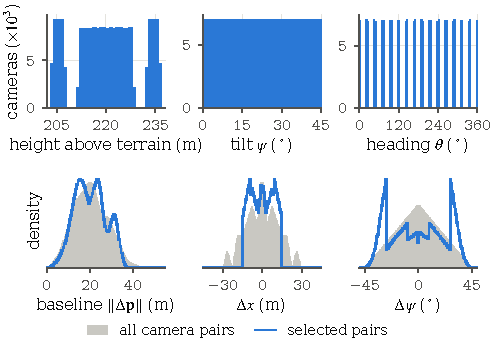
\includegraphics[width=\linewidth]{figures/fig_dataset.pdf}
\caption{\textbf{Camera and pair statistics of PairUAV.} Top: height above the terrain, tilt and heading of the cameras. Bottom: baseline length and pose differences of all camera pairs of a building (grey) and of the selected pairs (line).}
\label{fig:dataset}
\end{figure}

\subsection{Screening and selection of the pairs}

The 150 cameras of a building give \dsCand{} ordered pairs. The released pairs are obtained in three steps.

\noindent\textbf{Range.} All released pairs satisfy $|\Delta x|,|\Delta y|\le15$\,m, whereas the candidates reach 30\,m; the other three differences span the sampling ranges. \dsInRange\% of the candidate pairs lie within the ranges of the released ones.

\noindent\textbf{Visual screen.} Every released pair carries the statistics of an automatic screen, which we report from the metadata: SIFT matches filtered by a mutual ratio test, a fundamental matrix fitted with MAGSAC, the number of inliers, their ratio, the fraction of the image covered by their convex hull, and the number of occupied cells of a $4{\times}4$ grid. All released pairs have at least \dsMinInl{} inliers spread over at least \dsMinCells{} cells; the median pair has \dsInlMed{} inliers with an inlier ratio of \dsInlRatioMed, and \dsInlLtHundred\% of the pairs have fewer than 100 inliers (\cref{tab:dataset}). \todoauthors{Sec.~3.2 states that human annotators screened candidate pairs. Please provide the number of annotators, the agreement criterion, the number of candidate pairs shown and the rejection rate, and how the manual screen relates to the automatic one recorded in the metadata; none of this can be recovered from the released files, and we leave it blank rather than guess.}

\noindent\textbf{Balancing.} From the pairs that pass, 1{,}000 are selected per building, jointly over groups of five buildings (\dsGroups{} groups), with equal counts in five equal-width bins of each of the five pose differences. The released pairs are \dsSelFrac\% of all candidate pairs and \dsSelOfInRange\% of those within range. Their baselines range up to \dsDistMax\,m with a median of \dsDistMed\,m; 1\% are shorter than \dsDistPone\,m (\cref{tab:dataset}, \cref{fig:dataset}).

\subsection{Results on unscreened pairs}
\label{sec:unfiltered}

The reviews ask how the method performs on pairs that did not pass the selection. We use the \unN{} unscreened pairs of \cref{sec:unscreened}: four ordered pairs per test building, drawn uniformly from all $150{\times}149$ camera pairs, with labels recomputed from the camera poses. Of these pairs, \ufInX\% and \ufInY\% lie within the $\pm15$\,m of the released pairs in $\Delta x$ and in $\Delta y$ (\unInside\% in both), and our re-implementation of the visual screen, which accepts \ufProxyPass\% of the released pairs, accepts \unScreenPass\% of them.

\begin{table}[t]
\centering
\caption{\textbf{Unscreened pairs by overlap of the two ground footprints} (pairs of \cref{tab:unscreened}; refined stage unless stated, camera frame).}
\label{tab:overlap}
\footnotesize
\setlength{\tabcolsep}{4pt}
\begin{tabular}{@{}lccccc@{}}
\toprule
& Share & \SRd & \SRe & \SRe & EPE med. \\
Overlap & (\%) & (\%) & coarse & refined & (m) \\
\midrule
$<$ 0.02 & 23.1 & 7.8 & 0.4 & 0.4 & 21.32 \\
0.02-0.2 & 23.3 & 61.5 & 24.1 & 47.8 & 1.10 \\
0.2-0.4 & 24.0 & 80.9 & 68.7 & 78.8 & 0.53 \\
0.4-0.6 & 19.0 & 82.7 & 78.2 & 82.3 & 0.46 \\
$\geq$ 0.6 & 10.7 & 91.1 & 83.1 & 91.1 & 0.41 \\
\bottomrule
\end{tabular}
\end{table}


Over all unscreened pairs the refined stage reaches \unSiiSRd\% \SRd{} and \unSiiSRe\% \SRe{} in the camera frame (\cref{tab:unscreened}), against \SiiCamSRd\% and \SiiCamSRe\% on the released test pairs. On the unscreened pairs that lie within the released ranges and pass the screen it reaches \unInSiiSRd\% and \unInSiiSRe\%: the released pairs are representative of the pairs with these two properties, and the difference comes from the others. The decisive factor is the overlap of the two ground footprints (\cref{tab:overlap}). Pairs whose footprints overlap by less than 2\%, which are \unNoOverlap\% of all camera pairs of a building, cannot be solved by any method of \cref{tab:unscreened}; above 20\% of overlap the success is at the level of the released pairs; in between, the refinement doubles the endpoint success of the coarse stage. DreamNav returns an estimate for every pair, including those without common content. The numbers of the main paper therefore describe pairs that overlap, as its dataset section states, and a deployed system needs a test that rejects the others; the number of inliers, which is zero in the median for the pairs of the first row, is an obvious candidate that we have not evaluated.

\subsection{Release}

The footnote of the abstract commits to releasing the dataset and the code upon publication. The release will contain: the rendered images; the pose of every camera; the pair lists with their five labels and screening statistics, including the lists of unscreened pairs used in \cref{sec:unfiltered}; the building-level training and test splits; the evaluation code with the metric definitions of \cref{sec:metrics}, so that the range-based and the endpoint-based success rates are both reported; and the code and fitted models of DreamNav, including the scripts that produce every table of this document. \todoauthors{Please confirm the hosting, the licence of the rendered imagery, and whether the anonymised package can be linked for the reviewers.}

\section{Relation to concurrent last-meter work}
\label{sec:related}

One review lists seven recent works that the main paper does not discuss. We read all of them. Three address pose alignment on the two-parameter protocol of PairUAV used in the UAVM~2026 challenge~\cite{li2026lastmeter,liang2026rasr,zhou2026airalign}; four address neighbouring problems~\cite{deng2026anyimagenav,deng2026aeromap3d,zhu2026uanwm,sui2026protovisnav}. \Cref{tab:related} summarises them, and they will be discussed in the related work of the revised paper.

\begin{table*}[t]
\centering
\caption{\textbf{Concurrent works named by the reviewers.} ``Pair'': the method runs on one RGB image pair without other sensing.}
\label{tab:related}
\footnotesize
\setlength{\tabcolsep}{4pt}
\resizebox{\textwidth}{!}{%
\begin{tabular}{@{}l p{3.2cm} p{3.6cm} p{3.4cm} c p{3.9cm}@{}}
\toprule
Work & Task & Input & Output & Pair & Evaluation \\
\midrule
Li \etal~\cite{li2026lastmeter} & UAV pose alignment, 2 parameters & RGB pair, $512^2$, pitch fixed at $45^\circ$ & heading and range & \checkmark & PairUAV, two-parameter protocol; success at 10\,m \\
RASR~\cite{liang2026rasr} & same & RGB pair & heading and range, snapped to the label grid & \checkmark & UAVM~2026 leaderboard (relative errors) \\
AirAlign~\cite{zhou2026airalign} & same & RGB pair, $448^2$ & heading and signed range & \checkmark & UAVM~2026 leaderboard \\
\midrule
AnyImageNav~\cite{deng2026anyimagenav} & indoor image-goal navigation & RGB-D stream with odometry, keyframe history & 6-DoF pose of the goal image & -- & Habitat (Gibson, HM3D) \\
AeroMap3D~\cite{deng2026aeromap3d} & absolute UAV localization & RGB, satellite imagery, DEM, OSM & geo-referenced 6-DoF pose & -- & own flights; mean error 5.9\,m \\
UA-NWM~\cite{zhu2026uanwm} & long-range aerial image-goal navigation & RGB stream, goal image & cost of candidate trajectories & -- & AirSim; success at 20\,m \\
ProtoVis-Nav~\cite{sui2026protovisnav} & vision-language UAV navigation & RGB, instruction, state & next waypoint & -- & OpenUAV; success at 20\,m \\
\midrule
DreamNav (ours) & UAV pose alignment, 5-DoF & RGB pair, arbitrary heading, tilt $0^\circ$--$45^\circ$ & metric 3-D displacement, heading and tilt change & \checkmark & PairUAV (5-DoF), success at 1\,m; real photographs \\
\bottomrule
\end{tabular}}
\end{table*}

\noindent\textbf{The two-parameter protocol.} The benchmark of Li~\etal~\cite{li2026lastmeter}, used for the UAVM~2026 challenge~\cite{deuser2026uavm}, shares its name and its source buildings with ours but defines a different task: a method predicts the heading and the range between two of the 54 drone views of a University-1652 building~\cite{zheng2020university}, rendered at $512{\times}512$ pixels with a fixed pitch, and success is counted within 10\,m. The labels lie on a regular grid, and the challenge overview notes that several entries exploit this regularity~\cite{deuser2026uavm}; RASR, for instance, snaps its outputs to multiples of 2.5\,m and $20^\circ$~\cite{liang2026rasr}. The benchmark of this paper is its five-degree-of-freedom counterpart: 150 views per building with continuous positions, headings and tilts, labels in metres and degrees, and a success threshold of 1\,m. Scores on the two protocols are not comparable, and grid snapping has no equivalent here.

\noindent\textbf{What can be compared.} The leading entries of the challenge, including RASR and AirAlign, regress the two parameters from the features of a frozen 3-D reconstruction model (MASt3R, $\pi^3$, VGGT). We evaluate this design on our task in three ways. (i) The public pipeline of RASR, re-trained on our five labels, is the regression from pooled MASt3R statistics of \cref{tab:main_metrics}; it is also the first row of Table~3 of the main paper (\cref{sec:inventory}). It reaches a range error of 5.14\,m and a heading error of $5.7^\circ$, and \mlpCamD\,m and $1.8^\circ$ with the improved heads and a camera-frame target. (ii) AirAlign has no public implementation; its design, MLP heads on cached features of a frozen reconstruction model, belongs to the same family. (iii) The reconstruction models themselves, used as two-view pose estimators without any head, are evaluated in \cref{sec:geometric}. The outcome is consistent: regression from pooled features of a frozen geometric model reaches a few metres and a few degrees, which suits the two-parameter protocol, whereas the sub-metre, sub-degree regime of our benchmark requires correspondences.

\noindent\textbf{Diffusion-refined servoing.} The refinement stage of Li~\etal synthesises, with a pose-conditioned latent diffusion model at 512\,px, the views of a $3{\times}3$ grid of candidate poses spaced by $10^\circ$ in heading and 1.5 in range, and keeps the candidate whose synthesised view is closest to the target in pixel-wise error. On our benchmark the coarse stage is already accurate to $0.12^\circ$ and 0.9\,m, an order of magnitude finer than that candidate spacing. One metre of displacement moves the ground by 15 pixels in the full-resolution image and by 2 pixels at 512\,px, so that selecting between metre-level hypotheses requires the synthesised view to be geometrically exact to about one pixel. The control of \cref{sec:controls} that renders our geometrically exact warp at $512{\times}288$ gives an upper bound for an imagination of that resolution, whatever generates it: it yields \ctLowResSRd\% \SRd, below the \ctCoarseSRd\% of the coarse stage it starts from, against \ctFullSRd\% at the original resolution. \todoauthors{If the diffusion re-ranking experiment on top of our coarse stage is to be reported here, please add its protocol (model, candidate grid, number of test pairs); the result table on file shows all five errors increasing after re-ranking.}

\noindent\textbf{Neighbouring problems.} AnyImageNav~\cite{deng2026anyimagenav} registers a goal image to the observations of an indoor agent equipped with depth and odometry, using a history of keyframes to fix the metric scale; it shares our view of the goal image as a geometric query but does not apply to an isolated RGB pair. AeroMap3D~\cite{deng2026aeromap3d} localises a UAV in a geo-referenced map from satellite imagery, a terrain model and building footprints, with errors of several metres; such a system provides the coarse position from which a last-meter estimator starts. UA-NWM~\cite{zhu2026uanwm} plans long-range trajectories towards an image goal with a latent world model and counts success within 20\,m; it would hand over to a terminal estimator. ProtoVis-Nav~\cite{sui2026protovisnav} follows language instructions and has no goal image. We do not compare with these four methods because none of them outputs the relative pose of an image pair.

\section{Corrections and narrowed claims}
\label{sec:corrections}

Answering the reviews uncovered statements of the main paper that are imprecise, unsupported or wrong. We list them with the place where each is treated, so that the paper and this document can be read together without ambiguity. The numbers of Tables~2, 4 and~5 are reproduced exactly and do not change; one row of Table~3 changes; and several conclusions drawn from these tables have to be narrowed.

\begin{enumerate}[leftmargin=*,itemsep=2pt,topsep=3pt]
\item \textbf{Definition of the success rate (Sec.~5, ``Metrics'').} SR in Tables~2--4 thresholds the range error $d$, not the three-dimensional distance to the goal as the text says. Under the endpoint definition the refined stage succeeds on \SiiCamSRe\% of the pairs in the camera frame and \SiiEnuSRe\% in ENU, instead of 83.3\%; the coarse stage on \SiCamSRe\% and \SiEnuSRe\% (\cref{sec:whichdef}, \cref{tab:main_metrics}). Both definitions should be reported, and the headline number of the abstract should be accompanied by the endpoint success.
\item \textbf{The $d$ column} is the error of the predicted distance, not of the displacement vector (\cref{sec:whichdef}).
\item \textbf{Comparison with existing estimators (abstract, Sec.~1, Tables~2 and~4).} The eight baselines are navigation policies, world models and visual representations adapted to regress a relative pose, several of them with a linear probe or a single epoch (\cref{sec:baselines}); they are not ``widely used relative-pose regressors''. Against correspondence-based estimation the margin is small or negative: a SIFT pipeline with an essential matrix and the same flight-height prior reaches \sfSiftSRd\% / \sfSiftSRe\% (\SRd{} / \SRe) on the test pairs of Table~2, between our coarse stage (\sfSiSRd\% / \sfSiSRe\%) and our refined stage (\sfSiiSRd\% / \sfSiiSRe\%); RoMa with a rotation search is level with the refined stage on the pairs on which it was run; and on the real photographs both are more accurate than DreamNav (\grSiftSRe\% of endpoint success for the SIFT pipeline against \grSiiSRe\%; \cref{sec:geometric,sec:real}). These rows belong in Tables~2 and~4, and the claim of superiority should be restricted to the methods of Table~2 and to the refined stage on PairUAV.
\item \textbf{Table~3, first row.} ``Frozen SuperGlue'' is a regression from pooled MASt3R statistics and uses no correspondences (\cref{sec:inventory}).
\item \textbf{Table~3, third row.} ``+ absolute heading'' should read $d{=}$\fOneD\,m and SR${=}$\fOneSRd\%, not 2.25\,m and 35.1\%. Consequently the heading does not reduce the distance error, the zoom re-matching adds 8.0 points and not 38.0, and the corresponding sentences of Sec.~5.2 are withdrawn (\cref{sec:inventory}).
\item \textbf{Role of the plane-induced warp (title, abstract, Secs.~1 and~4.3).} The paper presents the ground-plane homography as what makes the refinement work. A compute-matched second matching pass that aligns the images by the coarse rotation only recovers \ctRotShareD\% of the gain in \SRd{} and \ctRotShareE\% of the gain in endpoint success; the plane-induced part adds \ctPlaneGainSRe{} points of endpoint success \ci{\ctPlaneGainSReLo}{\ctPlaneGainSReHi}, and the verification scores add nothing measurable. The contribution of the refinement stage should be described as pose-guided re-matching at the original resolution, of which the plane-induced warp is one, modestly better, form of alignment (\cref{sec:controls}).
\item \textbf{Abstract, internal \vs physical loop.} The increase from 38.8\% to 81.9\% is obtained with 2.2 \emph{physical} steps in simulation, each followed by a new rendered observation. The sentences ``Iterating the refinement 2.2 times [...] the loop closes inside the estimator rather than in the air'' conflate this with the internal refinement and are withdrawn. Repeating the refinement on a fixed pair, without moving, changes \SRe{} by \itThreeASRe{} \ci{\itThreeASReLo}{\itThreeASReHi} to \itThreeBSRe{} \ci{\itThreeBSReLo}{\itThreeBSReHi} points after three rounds, depending on the protocol (\cref{sec:iteration,sec:internalphysical}).
\item \textbf{Table~5, ``Ours (Stage~II)''.} This row uses, below 5\,m of estimated remaining distance, the ground-plane translation of \cref{sec:shortrange}, which the main paper does not describe. Averaged over \clSeeds{} draws of the actuation noise, the refined stage without it reaches \clSiiPlainSR\% at $\tau{=}1$\,m, against \clSiSR\% for the coarse stage and \clSiiSR\% with it: the gain of Table~5 comes from this solver and not from the refinement (\cref{sec:cluncertainty}). A classical image-based servo reaches \svIbvsFinal\% in the same simulator when it is given 20 steps (\cref{sec:servo}).
\item \textbf{Table~4, flight height.} The two DreamNav rows scale the predicted displacement by the ratio of the flight height reported by the aircraft (60\,m) to the height of the training data; the baselines receive no such input. Without the flight height the refined stage has a median position error of \rlNoHeightPos\,m (\cref{sec:real}).
\item \textbf{Sec.~5.3, ``generalizes well''.} This holds for the pairs of Table~4, whose baseline-to-height ratio lies within the training range, with the flight height given and in the camera frame. Beyond that range the endpoint success is \rlSiiOutSRe\%, and with the learned absolute heading it is \rlEnuSRe\% (\cref{sec:real}).
\item \textbf{``Unseen scenes'' and the ENU results.} The test pairs come from held-out \emph{buildings}, whose surroundings are not held out: the median test building stands \hdDistMedian\,m from a training building. The geometric part of the method is insensitive to this, but the learned absolute heading is not. On six sites removed entirely from the training of the heading network, the ENU endpoint success falls from \hdSdSeenSRe\% to \hdSdUnseenSRe\%, while the camera-frame success on the same pairs is \hdSdCamSRe\% (\cref{sec:headsite}); on the real photographs the heading prior is at $\hdRealFusedMed^\circ$ of median error (\cref{sec:headsens}). ``Unseen scenes'' should read ``unseen buildings'', the camera-frame results should be the primary ones, and the $\Delta x$, $\Delta y$ columns of Tables~2 and~3 should be presented as conditional on a heading prior that is specific to the sites of PairUAV. \todoauthors{Sec.~5 describes the split of the complete dataset, whereas the experiments of the paper and of this document use \nTest{} test pairs from \nBuildings{} held-out buildings and training pairs from 1{,}122 other buildings; please reconcile the two descriptions.}
\item \textbf{Sec.~4.2, absolute heading.} The refined output combines two heading networks, not one (\cref{sec:absh}).
\item \textbf{Eq.~(1).} The prior heading change in the last term lacks its bar (\cref{eq:map}).
\item \textbf{Figure~1 and the conclusion.} The experiments establish pose estimation from views taken about 220\,m above the ground and a simulated final approach without obstacles, dynamics or a flight controller. They do not establish close-range flight along a facade (\cref{sec:planarity}), obstacle avoidance, or deployment on an aircraft (\cref{sec:clscope}); the last sentence of the abstract and of the conclusion should be read as motivation.
\end{enumerate}

\noindent\textbf{Dependences that the paper should state.} (i) Metric scale relies on the regularity of the flight height in PairUAV, or on the flight height being given; this holds for our system and for every geometric baseline (\cref{sec:inventory,sec:georesults,sec:real}). (ii) The ENU output relies on an absolute heading learned from image appearance, which is accurate only near the training buildings and under the imaging conditions of the rendered imagery; the camera-frame output does not (\cref{sec:heading}). (iii) The calibration $K$, zero roll and tilts within $0^\circ$--$45^\circ$ are assumed (\cref{sec:conv,sec:coarse}). (iv) The pairs overlap: an estimate is returned for every pair, also for those without common content (\cref{sec:unfiltered}).

\noindent\textbf{What remains.} After these corrections the supported contributions are: the five-degree-of-freedom benchmark with metric labels; a pose-guided second matching pass at the original resolution that raises the endpoint success of a learned sparse matcher by \gainSReCam{} points and brings its translation direction to the level of a high-resolution classical pipeline; and a learned fusion of scale cues that estimates the distance better than a single flight-height cue on PairUAV (\cref{sec:georesults}). The same fusion does not transfer this advantage to the real photographs.


{
    \small
    \bibliographystyle{ieeenat_fullname}
    \bibliography{supp}
}
\end{document}
